\documentclass[11pt,a4paper]{article}
\usepackage[margin=2.2cm]{geometry}
\usepackage{lmodern}
\usepackage[T1]{fontenc}
\usepackage{microtype}
\usepackage{amsmath,amssymb,amsthm,bm,mathtools}
\usepackage{booktabs,array,tabularx}
\usepackage[dvipsnames]{xcolor}
\usepackage[most]{tcolorbox}
\usepackage{tikz}
\usetikzlibrary{arrows.meta,positioning,shapes.geometric,calc,matrix,fit,backgrounds,decorations.pathreplacing}
\usepackage{pgfplots}
\pgfplotsset{compat=1.18}
\usepackage{enumitem}
\usepackage[colorlinks=true,linkcolor=MidnightBlue,urlcolor=MidnightBlue,citecolor=MidnightBlue]{hyperref}
\setlength{\parskip}{4pt}\setlength{\parindent}{0pt}
\setlist{itemsep=2pt,topsep=3pt}

% ---------- boxes (same family as the DVS guide and the course book) ----------
\newtcolorbox{plainbox}{colback=blue!4,colframe=MidnightBlue,title=In plain words,fonttitle=\bfseries\small,boxrule=0.6pt,arc=2pt,breakable}
\newtcolorbox{watchbox}{colback=orange!6,colframe=BurntOrange,title=Watch out,fonttitle=\bfseries\small,boxrule=0.6pt,arc=2pt,breakable}
\newtcolorbox{examplebox}{colback=gray!6,colframe=gray!60,title=Worked example,fonttitle=\bfseries\small,boxrule=0.6pt,arc=2pt,breakable}
\newtcolorbox{whybox}{colback=violet!4,colframe=violet!60!black,title=Why it is true,fonttitle=\bfseries\small,boxrule=0.6pt,arc=2pt,breakable}
\newtcolorbox{algbox}[1][]{colback=white,colframe=black!50,title={#1},fonttitle=\bfseries\small,boxrule=0.6pt,arc=2pt,breakable}
\newtcolorbox{quizbox}{colback=yellow!7,colframe=olive!70!black,title=Check yourself,fonttitle=\bfseries\small,boxrule=0.6pt,arc=2pt,breakable}
\definecolor{addc}{HTML}{0f7b6c}
\definecolor{opc}{HTML}{b3261e}
\newtcolorbox{bridgebox}{colback=addc!5,colframe=addc,title={From your course book},fonttitle=\bfseries\small,boxrule=0.8pt,arc=2pt,breakable,leftrule=3pt}
\newtcolorbox{opinionbox}{colback=opc!4,colframe=opc,title={My assessment, not a published result},fonttitle=\bfseries\small,boxrule=0.8pt,arc=2pt,breakable,leftrule=3pt}
\newtcolorbox{probbox}[1]{colback=addc!6,colframe=addc!85!black,title={$\Sigma$\ \ Probability \& derivation: #1},fonttitle=\bfseries\small,boxrule=0.8pt,arc=2pt,breakable,leftrule=3pt}
\newtcolorbox{paperbox}[1]{colback=white,colframe=MidnightBlue!70,coltitle=white,colbacktitle=MidnightBlue!70,title={Paper card: #1},fonttitle=\bfseries\small,boxrule=0.6pt,arc=2pt,breakable}

\newcommand{\vect}[1]{\mathbf{#1}}
\newcommand{\R}{\mathbb{R}}
\newcommand{\x}{\vect{x}}
\newcommand{\w}{\vect{w}}
\newcommand{\h}{\vect{h}}
\newcommand{\y}{\vect{y}}
\newcommand{\z}{\vect{z}}
\newcommand{\s}{\vect{s}}
\newcommand{\av}{\vect{a}}
\newcommand{\E}{\mathbb{E}}
\DeclareMathOperator*{\argmin}{arg\,min}
\DeclareMathOperator*{\argmax}{arg\,max}
\DeclareMathOperator{\softmax}{softmax}

% ---------- palette ----------
\definecolor{cA}{HTML}{2a78d6}
\definecolor{cB}{HTML}{eb6834}
\definecolor{cC}{HTML}{1f9e89}
\definecolor{cD}{HTML}{7a4fb5}
\definecolor{inkm}{HTML}{52514e}
\definecolor{gridc}{HTML}{e1e0d9}

\pgfplotsset{
  every axis/.append style={axis lines=left, grid=major, grid style={gridc}, tick label style={font=\scriptsize,color=inkm},
     label style={font=\small}, title style={font=\small\bfseries}, legend style={font=\scriptsize,draw=none,fill=white,fill opacity=0.85,text opacity=1},
     width=7.2cm, height=5.2cm},
  cemcont/.style={color=gray!55, thin, no marks},
}
\tikzset{
  bx/.style={draw=inkm, rounded corners=2pt, fill=#1!9, align=center, font=\small, inner sep=4pt, minimum height=0.8cm},
  bx/.default=cA,
  arr/.style={-{Stealth[length=2mm]}, thick, color=inkm},
  darr/.style={-{Stealth[length=2mm]}, thick, dashed, color=cB},
  lbl/.style={font=\scriptsize, color=inkm, align=center},
  flowp/.style={color=inkm!55, thin},
}

\def\attaa{0.58}
\def\scaa{2.12}
\def\attab{0.11}
\def\scab{0.42}
\def\attac{0.07}
\def\scac{0.00}
\def\attad{0.25}
\def\scad{1.27}
\def\attba{0.25}
\def\scba{0.42}
\def\attbb{0.20}
\def\scbb{0.17}
\def\attbc{0.25}
\def\scbc{0.42}
\def\attbd{0.30}
\def\scbd{0.59}
\def\attca{0.06}
\def\scca{0.00}
\def\attcb{0.09}
\def\sccb{0.42}
\def\attcc{0.51}
\def\sccc{2.12}
\def\attcd{0.33}
\def\sccd{1.70}
\def\attda{0.19}
\def\scda{1.27}
\def\attdb{0.09}
\def\scdb{0.59}
\def\attdc{0.28}
\def\scdc{1.70}
\def\attdd{0.43}
\def\scdd{2.12}

\def\bimean{0.042}

\def\bandlo{-0.18}\def\bandhi{0.18}

\def\onestep{0.019}\def\errten{0.069}\def\errforty{0.259}

\def\cemmuxa{0.000}\def\cemmuya{0.000}
\def\cemmuxb{1.511}\def\cemmuyb{1.153}
\def\cemmuxc{1.599}\def\cemmuyc{1.200}
\def\cemfx{1.604}\def\cemfy{1.201}


\title{\textbf{Robots that Think and Imagine}\\[4pt]
\large Background notes on reasoning vision-language-action models and world models,\\ from linear regression to the research front\\[2pt]
\normalsize With a reading list, a map of the open problems for drones,\\ and every probability formula explained and derived}
\date{November 2026}

\begin{document}
\maketitle
\tableofcontents
\newpage

\section*{How to read these notes}
\addcontentsline{toc}{section}{How to read these notes}

These notes start where your machine-learning course ends: linear and logistic regression, gradient descent, bias and variance, and convolutional networks. They end at two research topics that are moving fast in 2025--2026:
\begin{itemize}
\item \textbf{Reasoning vision-language-action models (VLAs):} one network that looks at camera images, reads an instruction such as ``put the red cube in the box'', \emph{thinks in steps}, and outputs motor commands.
\item \textbf{World models:} a network that predicts what the robot will see and where it will be \emph{if} it takes a certain action, so the robot can try plans in imagination before it moves.
\end{itemize}
Figure~\ref{fig:roadmap} shows the dependency chain. Every arrow is a chapter you need before the next one. Parts I and II are background; Part III is VLAs; Part IV is world models; Part V puts them together for drones and gives the reading list.

\begin{figure}[h]
\centering
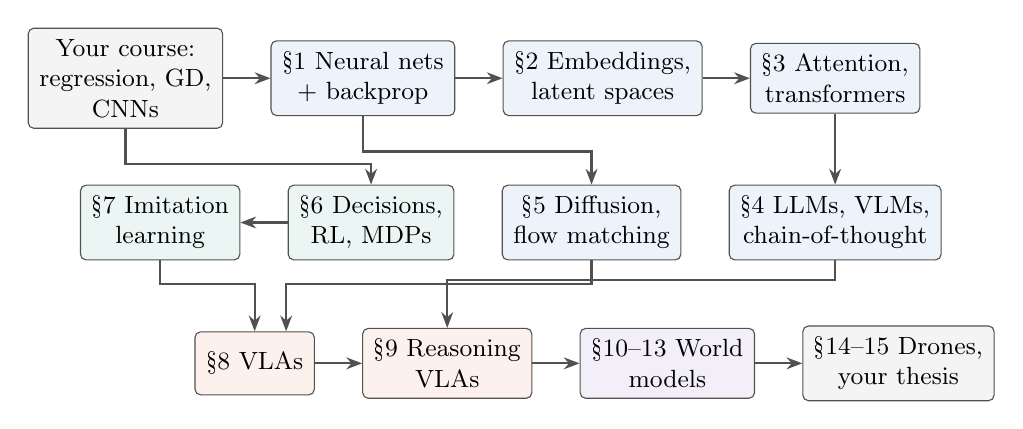
\begin{tikzpicture}[node distance=4mm and 6mm, every node/.style={font=\small}]
\node[bx=gray] (c) {Your course:\\regression, GD,\\CNNs};
\node[bx, right=of c] (nn) {\S1 Neural nets\\+ backprop};
\node[bx, right=of nn] (emb) {\S2 Embeddings,\\latent spaces};
\node[bx, right=of emb] (tr) {\S3 Attention,\\transformers};
\node[bx, below=9mm of tr] (llm) {\S4 LLMs, VLMs,\\chain-of-thought};
\node[bx, left=of llm] (gen) {\S5 Diffusion,\\flow matching};
\node[bx=cC, left=of gen] (rl) {\S6 Decisions,\\RL, MDPs};
\node[bx=cC, left=of rl] (il) {\S7 Imitation\\learning};
\node[bx=cB, below=9mm of il, xshift=12mm] (vla) {\S8 VLAs};
\node[bx=cB, right=of vla] (rvla) {\S9 Reasoning\\VLAs};
\node[bx=cD, right=of rvla] (wm) {\S10--13 World\\models};
\node[bx=gray, right=of wm] (you) {\S14--15 Drones,\\your thesis};
\draw[arr] (c)--(nn); \draw[arr] (nn)--(emb); \draw[arr] (emb)--(tr); \draw[arr] (tr)--(llm);
\draw[arr] (nn.south) |- ++(0,-0.45) -| (gen.north);
\draw[arr] (c.south) |- ++(0,-0.45) -| (rl.north);
\draw[arr] (rl)--(il);
\draw[arr] (il.south) -- ++(0,-0.3) -| (vla.north);
\draw[arr] (gen.south) |- ++(0,-0.3) -| ([xshift=4mm]vla.north);
\draw[arr] (llm.south) -- ++(0,-0.25) -| (rvla.north);
\draw[arr] (vla)--(rvla); \draw[arr] (rvla)--(wm); \draw[arr] (wm)--(you);
\end{tikzpicture}
\caption{Road map. Grey: what you already have and where you are going. Blue: deep-learning background. Green: robot-learning background. Orange: VLAs. Violet: world models.}
\label{fig:roadmap}
\end{figure}

\textbf{The boxes.} The box styles are the same as in your course book. Four are new:
\begin{bridgebox}
Links a new idea back to a chapter of the course book, so you can see that it is an old idea in new clothes.
\end{bridgebox}
\begin{opinionbox}
My own judgement or prediction, for example where I think the open research gaps are. Everything outside these boxes is either textbook material or what a cited paper reports.
\end{opinionbox}
\begin{paperbox}{Author et al.\ (year)}
A short summary of one paper: what problem, what idea, what result. The full list with arXiv numbers is in the Sources section at the end.
\end{paperbox}
\begin{probbox}{name of the idea}
Explains a probability or statistics idea the first time it is used, from zero, and derives the formula that appears in the text. Later chapters point back to these boxes instead of repeating them.
\end{probbox}

\textbf{About the numbers in the figures.} Every plot is drawn from small synthetic experiments that I ran for these notes (the script \texttt{make\_data.py} sits next to this file). They are toys, chosen so that you can redo every number by hand or in ten lines of NumPy. They are \emph{not} results from the papers.

\textbf{About the papers.} For papers from 2024 and earlier I describe what is well established. For the many 2026 papers in Part V I read the abstracts and summaries, not every page. Treat their numbers as ``what the authors report''.

% =====================================================================
\part{Deep-learning background}
% ============================== PART I ==============================
\section{From logistic regression to neural networks}

\subsection{A neuron is a logistic regression}
In the course you met logistic regression: take an input vector $\x$, compute a score $z=\w^\top\x+b$, and squash it with the sigmoid $\sigma(z)=1/(1+e^{-z})$ to get a probability. That \emph{is} one artificial neuron. A neural network is many of these, stacked so that the outputs of one layer are the inputs of the next:
\begin{equation}
\h_1=\phi(W_1\x+\vect{b}_1),\qquad \h_2=\phi(W_2\h_1+\vect{b}_2),\qquad \dots,\qquad \hat{\y}=W_L\h_{L-1}+\vect{b}_L .
\label{eq:mlp}
\end{equation}
$\phi$ is a non-linear activation, today almost always ReLU, $\max(0,z)$, or its smooth cousin GELU. Without $\phi$ the whole stack would collapse into one linear map $W_L\cdots W_1\x$, which is just linear regression again. The non-linearity is what lets the network bend its decision boundary.

\begin{probbox}{random variables, Bernoulli, and why the sigmoid gives a probability}
\textbf{Random variable.} A quantity whose value is uncertain, written with a capital letter, $Y$. Its \emph{distribution} says how likely each value is. A binary label $Y\in\{0,1\}$ (``cat or not'') has the \textbf{Bernoulli} distribution with one parameter $p=P(Y=1)$:
\[
P(Y=y)=p^{\,y}(1-p)^{1-y}\qquad(y=1\text{ gives }p,\quad y=0\text{ gives }1-p).
\]
\textbf{Conditional probability.} $P(A\mid B)=P(A\cap B)/P(B)$ is the probability of $A$ once we know that $B$ happened. A classifier models $P(Y=1\mid\x)$: the probability of the label \emph{given} the input.

\textbf{Odds and log-odds.} The odds are $p/(1-p)$: $p=0.8$ gives odds $4$ (``4 to 1''). The log-odds $\log\frac{p}{1-p}$ can be any real number, from $-\infty$ ($p\to0$) to $+\infty$ ($p\to1$), so it is a natural thing for a linear model to predict.

\textbf{Derivation of the sigmoid.} Logistic regression \emph{assumes} that the log-odds is linear in $\x$, $\log\frac{p}{1-p}=z=\w^\top\x+b$. Solve for $p$:
\[
\frac{p}{1-p}=e^{z}\ \Rightarrow\ p=e^{z}-p\,e^{z}\ \Rightarrow\ p\,(1+e^{z})=e^{z}\ \Rightarrow\ p=\frac{e^{z}}{1+e^{z}}=\frac{1}{1+e^{-z}}=\sigma(z).
\]
So the sigmoid is not an arbitrary squashing function: it is the inverse of the log-odds. Example: $z=\log 4\approx1.386$ gives $\sigma(z)=0.8$.
\end{probbox}

\begin{figure}[h]
\centering
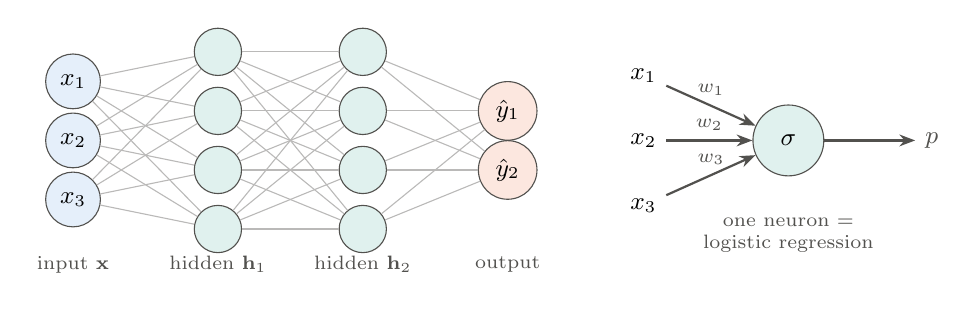
\begin{tikzpicture}[x=1.15cm,y=0.75cm, every node/.style={font=\small}]
\foreach \i in {1,2,3} \node[circle,draw=inkm,fill=cA!12,minimum size=6mm] (x\i) at (0,-\i) {$x_\i$};
\foreach \i in {1,...,4} \node[circle,draw=inkm,fill=cC!14,minimum size=6mm] (a\i) at (1.6,0.5-\i) {};
\foreach \i in {1,...,4} \node[circle,draw=inkm,fill=cC!14,minimum size=6mm] (b\i) at (3.2,0.5-\i) {};
\foreach \i in {1,2} \node[circle,draw=inkm,fill=cB!16,minimum size=6mm] (y\i) at (4.8,-0.5-\i) {$\hat y_\i$};
\foreach \i in {1,2,3} \foreach \j in {1,...,4} \draw[inkm!40] (x\i)--(a\j);
\foreach \i in {1,...,4} \foreach \j in {1,...,4} \draw[inkm!40] (a\i)--(b\j);
\foreach \i in {1,...,4} \foreach \j in {1,2} \draw[inkm!40] (b\i)--(y\j);
\node[lbl] at (0,-4.1) {input $\x$};
\node[lbl] at (1.6,-4.1) {hidden $\h_1$};
\node[lbl] at (3.2,-4.1) {hidden $\h_2$};
\node[lbl] at (4.8,-4.1) {output};
\begin{scope}[shift={(7.9,-2)}]
\node[circle,draw=inkm,fill=cC!14,minimum size=9mm] (n) at (0,0) {$\sigma$};
\foreach \i/\yy in {1/1.1,2/0,3/-1.1} {\node[font=\small] (xi\i) at (-1.6,\yy) {$x_\i$}; \draw[arr] (xi\i)--(n) node[midway,above,font=\scriptsize]{$w_\i$};}
\draw[arr] (n)--(1.4,0) node[right,font=\small]{$p$};
\node[lbl] at (0,-1.6) {one neuron $=$\\logistic regression};
\end{scope}
\end{tikzpicture}
\caption{A multilayer perceptron (MLP) with two hidden layers (left). Every circle in the middle computes what the single neuron on the right computes: a weighted sum followed by a non-linearity.}
\label{fig:mlp}
\end{figure}

\begin{bridgebox}
Course book, logistic regression and the MLP section of the CNN chapter. A CNN is an MLP whose first layers share weights across image positions. Everything below about training applies to both.
\end{bridgebox}

\subsection{The loss is a negative log-likelihood}
Every loss you will see in these notes comes from one recipe: \emph{make the observed data as probable as possible under the model}. Write the model as a probability distribution $p_\theta(y\mid\x)$ with parameters $\theta$ and minimise
\begin{equation}
\mathcal L(\theta) = -\frac1N\sum_{n=1}^N \log p_\theta(y_n\mid \x_n).\label{eq:nll}
\end{equation}
\begin{itemize}
\item If the model says $y$ is Gaussian around $\hat y$ with fixed variance, $-\log p$ is $(y-\hat y)^2$ up to constants: the \textbf{mean squared error} from regression.
\item If $y$ is one of $K$ classes and the model outputs probabilities $p_1,\dots,p_K$, $-\log p$ is $-\log p_{y}$: the \textbf{cross-entropy} from classification.
\end{itemize}

\begin{probbox}{likelihood, independence, and where MSE and cross-entropy come from}
\textbf{Independence.} Two events are independent if knowing one does not change the other: $P(A\cap B)=P(A)P(B)$. We assume the training examples are \emph{independent and identically distributed} (i.i.d.): drawn separately from the same distribution. Then the probability of the whole dataset is a product:
\[
P(y_1,\dots,y_N\mid\x_1,\dots,\x_N)=\prod_{n=1}^N p_\theta(y_n\mid\x_n)\ =:\ \mathcal{L}ik(\theta).
\]
Read as a function of the parameters $\theta$, this product is the \textbf{likelihood}. \textbf{Maximum likelihood} picks the $\theta$ that makes the observed data most probable.

\textbf{Why the log.} $\log$ is increasing, so maximising $\log\mathcal Lik$ gives the same $\theta$. It turns the product into a sum, $\log\prod_n p_n=\sum_n\log p_n$, which is easy to differentiate, and it avoids numerical underflow (a product of a million numbers below 1 is 0 in floating point). Negating and dividing by $N$ gives equation~\eqref{eq:nll}: minimise the average negative log-likelihood.

\textbf{Densities.} For a continuous $y$, $p(y)$ is a \emph{density}: probabilities are areas under it, $P(a\le Y\le b)=\int_a^b p(y)\,\mathrm dy$, and $p(y)$ itself may exceed 1.

\textbf{Derivation 1: Gaussian $\Rightarrow$ MSE.} The Gaussian (normal) density with mean $\hat y$ and variance $\sigma^2$ is
\[
\mathcal N(y;\hat y,\sigma^2)=\frac{1}{\sqrt{2\pi\sigma^2}}\exp\!\Big(-\frac{(y-\hat y)^2}{2\sigma^2}\Big),
\qquad
-\log\mathcal N=\frac{(y-\hat y)^2}{2\sigma^2}+\tfrac12\log(2\pi\sigma^2).
\]
With $\sigma$ fixed, the second term is a constant and the first is the squared error times $1/(2\sigma^2)$. Same minimiser as MSE.

\textbf{Derivation 2: Bernoulli $\Rightarrow$ binary cross-entropy.} $-\log\big[p^{\,y}(1-p)^{1-y}\big]=-y\log p-(1-y)\log(1-p)$.

\textbf{Derivation 3: categorical $\Rightarrow$ cross-entropy.} With $K$ classes, $P(Y=k)=p_k$. Writing the label as a one-hot vector $\vect t$, $-\log p_y=-\sum_k t_k\log p_k$, because only the true class has $t_k=1$.
\end{probbox}
This matters later. A language model is a classifier over a vocabulary of about $10^5$ tokens, trained with cross-entropy. A VLA that writes actions as tokens is the same classifier. A diffusion policy is trained with a squared error that comes from a Gaussian.

\subsection{Backpropagation is the chain rule, done in the right order}
Gradient descent needs $\partial\mathcal L/\partial\theta$ for millions of parameters. Backpropagation computes all of them in one backward sweep, at about the cost of one forward pass. Draw the computation as a graph, go forward once and store every intermediate value, then go backward and multiply local derivatives.

\begin{figure}[h]
\centering
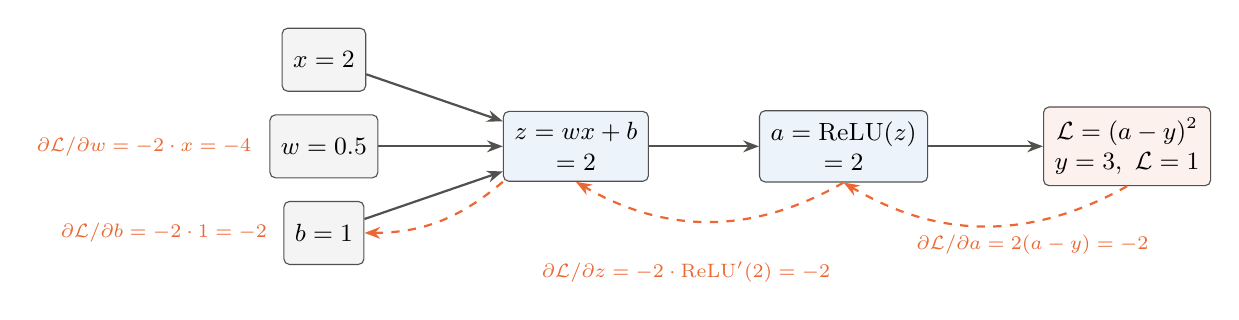
\begin{tikzpicture}[every node/.style={font=\small}]
\node[bx=gray] (x) at (0,1.1) {$x=2$};
\node[bx=gray] (w) at (0,0) {$w=0.5$};
\node[bx=gray] (b) at (0,-1.1) {$b=1$};
\node[bx] (z) at (3.2,0) {$z=wx+b$\\$=2$};
\node[bx] (a) at (6.6,0) {$a=\mathrm{ReLU}(z)$\\$=2$};
\node[bx=cB] (L) at (10.2,0) {$\mathcal L=(a-y)^2$\\$y=3,\ \mathcal L=1$};
\draw[arr] (x)--(z); \draw[arr] (w)--(z); \draw[arr] (b)--(z); \draw[arr] (z)--(a); \draw[arr] (a)--(L);
\draw[darr] (L.south) to[bend left=30] (a.south);
\draw[darr] (a.south) to[bend left=30] (z.south);
\draw[darr] (z.south west) to[bend left=20] (b.east);
\node[font=\scriptsize,color=cB,align=center] at (9.0,-1.25) {$\partial\mathcal L/\partial a=2(a-y)=-2$};
\node[font=\scriptsize,color=cB,align=center] at (4.6,-1.6) {$\partial\mathcal L/\partial z=-2\cdot\mathrm{ReLU}'(2)=-2$};
\node[font=\scriptsize,color=cB,anchor=east,align=right] at (-0.8,0) {$\partial\mathcal L/\partial w=-2\cdot x=-4$};
\node[font=\scriptsize,color=cB,anchor=east,align=right] at (-0.6,-1.1) {$\partial\mathcal L/\partial b=-2\cdot1=-2$};
\end{tikzpicture}
\caption{Backpropagation on a one-neuron network. Black: the forward pass, which stores every value. Orange dashed: the backward pass, which multiplies local derivatives from the loss back to each parameter.}
\label{fig:backprop}
\end{figure}

\begin{examplebox}
In Figure~\ref{fig:backprop} the prediction is $a=2$ but the target is $y=3$, so the loss is $1$. Both gradients are negative, so gradient descent \emph{increases} $w$ and $b$. With step size $\eta=0.1$: $w\leftarrow 0.5+0.4=0.9$ and $b\leftarrow 1+0.2=1.2$. The new prediction is $0.9\cdot2+1.2=3.0$, exactly the target. (A lucky step. Usually it only gets closer.)
\end{examplebox}

Libraries such as PyTorch and JAX build this graph automatically (\emph{autograd}). You write the forward pass; they give you the gradients.

\subsection{Optimisers and the tricks that make deep nets train}
Plain gradient descent from the course becomes, in practice:
\begin{itemize}
\item \textbf{Mini-batch SGD:} estimate the gradient from a random batch of 32--4096 examples instead of the whole dataset (the course's stochastic gradient descent).
\item \textbf{Adam} (Kingma \& Ba, 2015): keep a running mean $m$ of the gradients and a running mean $v$ of their squares, and step by $\eta\, m/(\sqrt v+\epsilon)$. Every parameter gets its own step size. Adam (or its variant AdamW, with weight decay) trains almost every model in these notes.
\item \textbf{Residual connections} (He et al., 2016): compute $\h_{l+1}=\h_l+f(\h_l)$ instead of $\h_{l+1}=f(\h_l)$. The gradient then has a direct path back through the ``$+$'', so networks with a hundred layers still train. Every transformer uses them.
\item \textbf{Normalisation layers} (batch norm, layer norm): rescale activations to mean $0$ and variance $1$ so that they stay in a good range for the next layer.
\item \textbf{Regularisation:} weight decay is the L2 penalty from the course; dropout randomly switches off units during training.
\end{itemize}

\begin{probbox}{expectation, the law of large numbers, and why mini-batches work}
\textbf{Expectation.} The expected value is the probability-weighted average: $\E[f(X)]=\sum_x P(x)f(x)$ for discrete $X$, or $\int p(x)f(x)\,\mathrm dx$ for continuous $X$. It is \emph{linear}: $\E[aX+bY]=a\E[X]+b\E[Y]$, always, even if $X$ and $Y$ are dependent. The \textbf{variance} $\mathrm{Var}(X)=\E[(X-\E X)^2]=\E[X^2]-(\E X)^2$ measures spread; $\mathrm{Var}(cX)=c^2\mathrm{Var}(X)$, and for \emph{independent} $X,Y$, $\mathrm{Var}(X+Y)=\mathrm{Var}(X)+\mathrm{Var}(Y)$.

\textbf{Law of large numbers.} The average of many i.i.d.\ samples approaches the expectation. That is why the training loss $\frac1N\sum_n\ell_n$ is a stand-in for the expected loss on new data.

\textbf{Mini-batch gradients are unbiased.} Let the full gradient be $\vect g=\frac1N\sum_{n=1}^N\nabla\ell_n$. Draw one index $i$ uniformly at random. Then
\[
\E[\nabla\ell_i]=\sum_{n=1}^N\tfrac1N\nabla\ell_n=\vect g .
\]
A batch of $B$ such draws averages $B$ unbiased estimates, so it is unbiased too, and (by the variance rules above) its variance is $\mathrm{Var}(\nabla\ell_i)/B$. Bigger batches give less noisy steps, but the noise falls only like $1/\sqrt B$ in standard deviation: 4 times the batch for half the noise.
\end{probbox}

\begin{watchbox}
The bias--variance story from the course still holds, but with a twist: very large networks trained on very large data often keep improving as they grow, instead of overfitting. This is why ``bigger model, more data'' has dominated since about 2020. It does not hold when the data is small. Most robot datasets \emph{are} small, which is one reason robotics borrows models pretrained on internet data.
\end{watchbox}

\begin{quizbox}
\begin{enumerate}[leftmargin=*]
\item Why does a network without activation functions reduce to linear regression?
\item Which loss do you get from the negative log-likelihood if the model outputs a Laplace distribution, $p(y)\propto e^{-|y-\hat y|}$?
\item In Figure~\ref{fig:backprop}, what are the gradients if $x=-1$ (so $z=0.5$)?
\end{enumerate}
\emph{Answers: 1) a product of matrices is a matrix; 2) the absolute error $|y-\hat y|$; 3) $a=0.5$, $\partial\mathcal L/\partial a=-5$, $\partial\mathcal L/\partial w=+5$, $\partial\mathcal L/\partial b=-5$.}
\end{quizbox}

% --------------------------------------------------------------------
\section{Embeddings and latent spaces}

\subsection{Turning symbols into vectors}
A network can only multiply numbers. Words, image patches and robot actions must become vectors first. The naive way is one-hot encoding: word number $i$ out of $V$ becomes a vector of length $V$ with a single 1. That is huge and says nothing about meaning. Instead, every model in these notes uses an \textbf{embedding table}: a learned matrix $E\in\R^{V\times d}$, and token $i$ becomes row $E_i$, a dense vector with $d$ between 256 and 8192. The rows are trained by backpropagation like any other weight, and similar tokens end up close together.

\textbf{Tokens.} Text is cut into pieces called tokens by a \emph{tokenizer}. Common words are one token; rare words are split into several (``quadrotor'' might be ``quad'' + ``rotor''). A typical vocabulary has 32\,000 to 256\,000 tokens. VLAs later add special tokens for actions.

\subsection{Latent spaces and autoencoders}
An \textbf{autoencoder} squeezes an input through a narrow middle layer and is trained to reconstruct it:
\begin{equation}
\z=\mathrm{enc}(\x)\in\R^{d_z},\qquad \hat\x=\mathrm{dec}(\z),\qquad \mathcal L=\lVert \x-\hat\x\rVert^2,\qquad d_z\ll \dim\x .
\end{equation}
Because $\z$ is small, the encoder must keep only what matters. The space where $\z$ lives is called the \textbf{latent space}. A $64\times64$ camera image has 12\,288 numbers; a good latent might have 32--1024. World models (Part IV) almost never predict pixels directly. They predict the next \emph{latent}, which is far cheaper.

A \textbf{variational autoencoder} (VAE) makes the latent a probability distribution: the encoder outputs a mean and a variance, $\z$ is sampled from it, and an extra KL term in the loss keeps these distributions close to a standard Gaussian. This makes the latent space smooth, so that you can sample new $\z$ and decode them. The first world model (Ha \& Schmidhuber, 2018) used exactly a VAE as its ``eyes''.

\begin{probbox}{KL divergence, the Gaussian KL, and sampling with gradients}
\textbf{KL divergence} measures how different a distribution $q$ is from a distribution $p$:
\[
\mathrm{KL}(q\,\|\,p)=\E_{z\sim q}\Big[\log\frac{q(z)}{p(z)}\Big]=\int q(z)\log\frac{q(z)}{p(z)}\,\mathrm dz .
\]
It is $0$ only when $q=p$, otherwise positive, and it is not symmetric ($\mathrm{KL}(q\|p)\ne\mathrm{KL}(p\|q)$). \emph{Why it is never negative:} $\log$ is concave, so Jensen's inequality says $\E[\log X]\le\log\E[X]$. Hence $-\mathrm{KL}=\E_q[\log\tfrac pq]\le\log\E_q[\tfrac pq]=\log\int q\,\tfrac pq=\log\int p=\log1=0$.

\textbf{Derivation: KL between a Gaussian and the standard Gaussian} (what the VAE loss uses). Let $q=\mathcal N(\mu,s^2)$ and $p=\mathcal N(0,1)$. From the density formula,
\[
\log q(z)-\log p(z)=-\tfrac12\log s^2-\frac{(z-\mu)^2}{2s^2}+\frac{z^2}{2}.
\]
Take the expectation under $q$, using $\E_q[(z-\mu)^2]=s^2$ and $\E_q[z^2]=\mathrm{Var}+\text{mean}^2=s^2+\mu^2$:
\[
\mathrm{KL}(q\|p)=-\tfrac12\log s^2-\tfrac12+\tfrac12(s^2+\mu^2)=\tfrac12\big(\mu^2+s^2-1-\log s^2\big).
\]
It is zero exactly when $\mu=0$ and $s=1$. For a $d$-dimensional latent with independent coordinates, add the $d$ terms.

\textbf{The reparameterisation trick.} We cannot backpropagate through ``draw a random sample''. Instead write $z=\mu+s\,\epsilon$ with $\epsilon\sim\mathcal N(0,1)$. By linearity, $\E[z]=\mu$ and $\mathrm{Var}(z)=s^2\mathrm{Var}(\epsilon)=s^2$, so $z$ has the right distribution; and now $z$ is a differentiable function of $\mu$ and $s$, with the randomness moved into $\epsilon$. Section~\ref{sec:dreamer} derives the full VAE loss (the ELBO).
\end{probbox}

\begin{figure}[h]
\centering
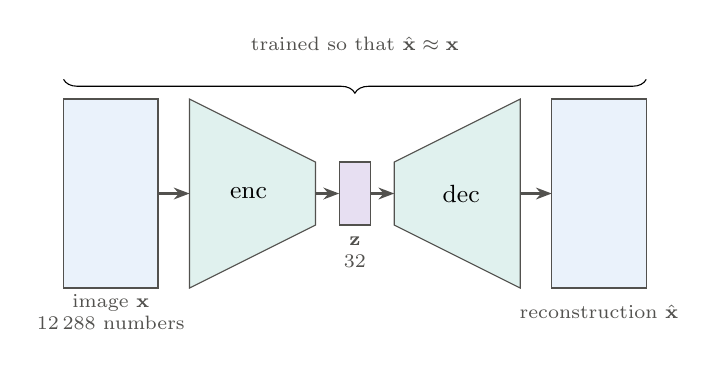
\begin{tikzpicture}[every node/.style={font=\small}]
\draw[fill=cA!10,draw=inkm] (0,1.2) rectangle (1.2,-1.2); \node[lbl] at (0.6,-1.5) {image $\x$\\12\,288 numbers};
\draw[fill=cC!14,draw=inkm] (1.6,1.2) -- (3.2,0.4) -- (3.2,-0.4) -- (1.6,-1.2) -- cycle; \node at (2.35,0) {enc};
\draw[fill=cD!18,draw=inkm] (3.5,0.4) rectangle (3.9,-0.4); \node[lbl] at (3.7,-0.75) {$\z$\\32};
\draw[fill=cC!14,draw=inkm] (4.2,0.4) -- (5.8,1.2) -- (5.8,-1.2) -- (4.2,-0.4) -- cycle; \node at (5.05,0) {dec};
\draw[fill=cA!10,draw=inkm] (6.2,1.2) rectangle (7.4,-1.2); \node[lbl] at (6.8,-1.5) {reconstruction $\hat\x$};
\draw[arr] (1.2,0)--(1.6,0); \draw[arr] (3.2,0)--(3.5,0); \draw[arr] (3.9,0)--(4.2,0); \draw[arr] (5.8,0)--(6.2,0);
\draw[decorate,decoration={brace,amplitude=5pt}] (7.4,1.45) -- (0,1.45) ;
\node[lbl] at (3.7,1.9) {trained so that $\hat\x\approx\x$};
\end{tikzpicture}
\caption{An autoencoder. The narrow middle forces the network to keep only the information needed to rebuild the image. The space of $\z$ is the latent space.}
\end{figure}

\subsection{Contrastive learning: matching images and text}
How do you get an image embedding that ``means'' the same as a sentence? \textbf{CLIP} (Radford et al., 2021) trained an image encoder and a text encoder on 400 million image--caption pairs from the internet. In a batch of $N$ pairs, it computes all $N^2$ similarities $s_{ij}=\langle \z^{\text{img}}_i,\z^{\text{txt}}_j\rangle$ (after normalising the vectors) and treats each row as an $N$-way classification whose correct answer is the diagonal:
\begin{equation}
\mathcal L_i=-\log\frac{e^{s_{ii}/\tau}}{\sum_{j=1}^N e^{s_{ij}/\tau}} \qquad\text{(and the same for columns).}
\end{equation}
This is the softmax cross-entropy from the course, where the ``classes'' are the other captions in the batch. SigLIP (Zhai et al., 2023) replaces the softmax with independent sigmoids and is the image encoder inside several VLAs. \textbf{DINOv2} (Oquab et al., 2023) learns image features without any text, by making two augmented views of the same image produce similar features. Its features are so good at geometry that DINO-WM (Section~\ref{sec:latentplan}) builds a world model directly on top of them.

\begin{probbox}{the softmax is a categorical distribution, and its gradient}
\textbf{Definition.} For scores (logits) $s_1,\dots,s_K$, $\ \softmax_k(\vect s)=\dfrac{e^{s_k}}{\sum_j e^{s_j}}$. Every entry is positive and they sum to 1, so the result is a valid \textbf{categorical distribution}: the probability of class $k$.

\textbf{Two classes give the sigmoid.} $\dfrac{e^{s_1}}{e^{s_1}+e^{s_2}}=\dfrac{1}{1+e^{-(s_1-s_2)}}=\sigma(s_1-s_2)$ (divide top and bottom by $e^{s_1}$). Softmax is the multi-class logistic regression.

\textbf{Shift invariance.} Adding the same $c$ to every score multiplies top and bottom by $e^{c}$, which cancels. Libraries subtract $\max_j s_j$ before exponentiating so that $e^{s}$ never overflows.

\textbf{Derivation of the gradient.} The cross-entropy for true class $y$ is $-\log\softmax_y=-s_y+\log\sum_j e^{s_j}$. Differentiate with respect to $s_k$:
\[
\frac{\partial}{\partial s_k}\Big(-s_y+\log\sum_j e^{s_j}\Big)=-\mathbb 1[k=y]+\frac{e^{s_k}}{\sum_j e^{s_j}}=p_k-\mathbb 1[k=y].
\]
``Predicted probability minus target'': it pushes the true class up and every other class down in proportion to how much probability it wrongly took. This one line is the training signal of CLIP, of every LLM and of every token-based VLA.

\textbf{Temperature.} Dividing the scores by $\tau$ (or $T$) before the softmax: as $\tau\to0$ the largest score takes all the probability (a one-hot vector); as $\tau\to\infty$ all classes become equally likely.
\end{probbox}

\begin{figure}[h]
\centering
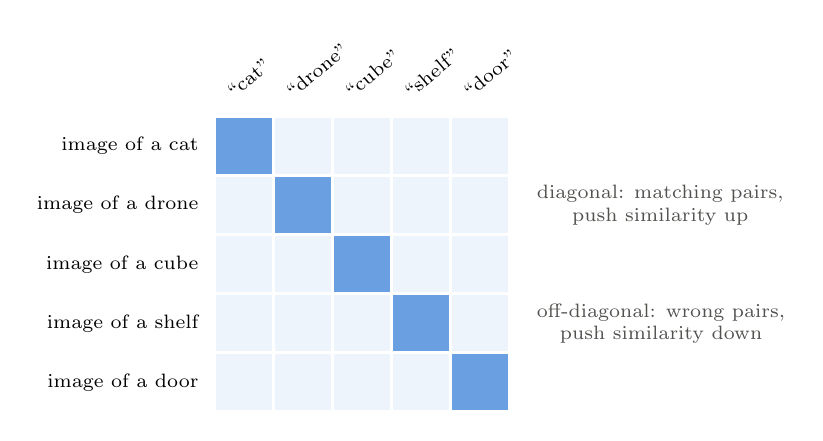
\begin{tikzpicture}[x=0.75cm,y=0.75cm,every node/.style={font=\scriptsize}]
\foreach \i in {0,...,4} \foreach \j in {0,...,4} {
  \ifnum\i=\j \fill[cA!70] (\j,-\i) rectangle ++(1,-1); \else \fill[cA!8] (\j,-\i) rectangle ++(1,-1); \fi
  \draw[white,line width=1pt] (\j,-\i) rectangle ++(1,-1);}
\foreach \t [count=\j from 0] in {cat,drone,cube,shelf,door} \node[rotate=40,anchor=south west] at (\j+0.3,0.05) {``\t''};
\foreach \t [count=\i from 0] in {cat,drone,cube,shelf,door} \node[anchor=east] at (-0.1,-\i-0.5) {image of a \t};
\node[lbl,anchor=west] at (5.3,-1.5) {diagonal: matching pairs,\\push similarity up};
\node[lbl,anchor=west] at (5.3,-3.5) {off-diagonal: wrong pairs,\\push similarity down};
\end{tikzpicture}
\caption{Contrastive training in CLIP. Each row is a classification over the captions in the batch, and the correct class is the diagonal.}
\end{figure}

\begin{quizbox}
\begin{enumerate}[leftmargin=*]
\item Why is a 32-number latent more useful for planning than the 12\,288 raw pixels?
\item In CLIP, what plays the role of the ``class labels'' in the cross-entropy?
\end{enumerate}
\emph{Answers: 1) predicting 32 numbers ahead is cheap and focuses on what matters, not on every pixel of texture; 2) the indices of the matching captions within the batch.}
\end{quizbox}

% --------------------------------------------------------------------
\section{Attention and the transformer}
\label{sec:transformer}

\subsection{The problem: sequences of any length}
An MLP takes a fixed-size input. A sentence, a video or a robot trajectory is a \emph{sequence} of variable length, and the meaning of one element depends on the others: in ``pick the red cube'', the word ``cube'' needs ``red'' to know which cube. Before 2017 the standard answer was the \textbf{recurrent neural network} (RNN, and its improved form the LSTM): read the sequence one step at a time and carry a hidden state $\h_t=f(\h_{t-1},\x_t)$. RNNs are slow to train because step $t$ waits for step $t-1$, and information from far back fades. They come back in Part IV, because a world model that steps forward in time is naturally recurrent.

\subsection{Attention: a soft dictionary lookup}
Attention lets every element look directly at every other element. Each token $i$ produces three vectors from its embedding $\x_i$:
\begin{align*}
\vect q_i&=W_Q\x_i && \text{query: what am I looking for?}\\
\vect k_i&=W_K\x_i && \text{key: what do I offer?}\\
\vect v_i&=W_V\x_i && \text{value: what I pass on.}
\end{align*}
Token $i$ scores every token $j$ by how well its query matches their key, turns the scores into weights with a softmax, and takes the weighted average of the values:
\begin{equation}
\alpha_{ij}=\softmax_j\!\left(\frac{\vect q_i^\top\vect k_j}{\sqrt{d_k}}\right),\qquad
\vect o_i=\sum_j\alpha_{ij}\,\vect v_j .
\label{eq:attn}
\end{equation}
In matrix form, with one row per token, this is $\mathrm{Attention}(Q,K,V)=\softmax\!\big(QK^\top/\sqrt{d_k}\big)\,V$.
The division by $\sqrt{d_k}$ keeps the scores from growing with the vector length; otherwise the softmax saturates and its gradients vanish.

\begin{probbox}{why divide by $\sqrt{d_k}$: the variance of a dot product}
Assume the components $q_m$ and $k_m$ of a query and a key are independent, with mean 0 and variance 1 (roughly true at initialisation). The score is $\vect q^\top\vect k=\sum_{m=1}^{d_k}q_mk_m$.
\begin{itemize}[leftmargin=*]
\item One term: $\E[q_mk_m]=\E[q_m]\E[k_m]=0$ (for independent variables the expectation of a product is the product of expectations), and $\mathrm{Var}(q_mk_m)=\E[q_m^2k_m^2]-0=\E[q_m^2]\E[k_m^2]=1\cdot1=1$.
\item The sum of $d_k$ independent terms: variances add, so $\mathrm{Var}(\vect q^\top\vect k)=d_k$ and the standard deviation is $\sqrt{d_k}$.
\item Dividing by $\sqrt{d_k}$: $\mathrm{Var}\big(\vect q^\top\vect k/\sqrt{d_k}\big)=d_k/d_k=1$, whatever the dimension.
\end{itemize}
With $d_k=64$ and no scaling, typical scores would be about $\pm8$; $e^{8}\approx3000$ times $e^{0}$, so the softmax would put almost all weight on one token and its gradient (box above: $p_k-\mathbb 1[k=y]$-type terms with $p$ near 0 or 1) would be almost zero.
\end{probbox}

\begin{examplebox}
Four tokens with 2-D embeddings: pick $=(1,0)$, the $=(0.2,0.2)$, red $=(0,1)$, cube $=(0.6,0.8)$. Take $W_Q=2I$ and $W_K=1.5I$. The query of ``cube'' is $(1.2,1.6)$ and the keys are $(1.5,0)$, $(0.3,0.3)$, $(0,1.5)$, $(0.9,1.2)$. The dot products divided by $\sqrt2$ are
\[
\scda,\quad \scdb,\quad \scdc,\quad \scdd .
\]
The softmax turns them into the weights $\attda,\ \attdb,\ \attdc,\ \attdd$. So the output for ``cube'' is mostly its own value plus a large share of ``red'' (\attdc) and very little of ``the'' (\attdb). That is how ``cube'' becomes ``red cube''. Figure~\ref{fig:attn} shows all sixteen weights.
\end{examplebox}

\begin{figure}[h]
\centering
\begin{tikzpicture}
\begin{axis}[width=6.3cm,height=6.3cm,enlargelimits=false,axis lines=box,grid=none,
  colormap={bl}{color=(white) color=(cA)}, point meta min=0, point meta max=0.65,
  xtick={0,1,2,3}, xticklabels={pick,the,red,cube}, ytick={0,1,2,3}, yticklabels={pick,the,red,cube},
  y dir=reverse, xlabel={key token $j$ (looked at)}, ylabel={query token $i$ (looking)},
  nodes near coords={\pgfmathprintnumber[fixed,precision=2]\pgfplotspointmeta}, every node near coord/.append style={font=\scriptsize,anchor=center,color=black},
  tick label style={font=\small,color=black}]
\addplot[matrix plot*, mesh/cols=4, point meta=explicit] table[meta=w]{figs/attn.dat};
\end{axis}
\end{tikzpicture}
\caption{Attention weights $\alpha_{ij}$ for the worked example. Each row sums to 1. Row ``cube'' puts weight on ``red'', which is how context flows between tokens.}
\label{fig:attn}
\end{figure}

\textbf{Multi-head attention} runs $h$ attentions in parallel with different $W_Q,W_K,W_V$ (for example one head can track colour words, another spatial words) and concatenates the outputs. \textbf{Self-attention} means queries, keys and values all come from the same sequence. \textbf{Cross-attention} means the queries come from one sequence (say, action tokens) and keys and values from another (say, image tokens). VLAs use both.

\subsection{Position and causality}
Equation~\eqref{eq:attn} treats the tokens as a set: shuffle them and each output is the same. Order is added by a \textbf{positional encoding}, a vector added to each embedding that depends on its position (sinusoids in the original paper, rotary encodings in most modern models). For generation, a \textbf{causal mask} sets $\alpha_{ij}=0$ for $j>i$, so that a token can only look at the past. This is what lets a model be trained on all positions of a sequence at once and still generate one token at a time.

\subsection{The transformer block}
A transformer (Vaswani et al., 2017) is a stack of identical blocks. Each block is attention followed by a small MLP, each wrapped in a residual connection and a layer norm (Figure~\ref{fig:block}). The attention mixes information \emph{between} tokens; the MLP processes each token \emph{on its own}. Large models stack 24--100 such blocks.

\begin{figure}[h]
\centering
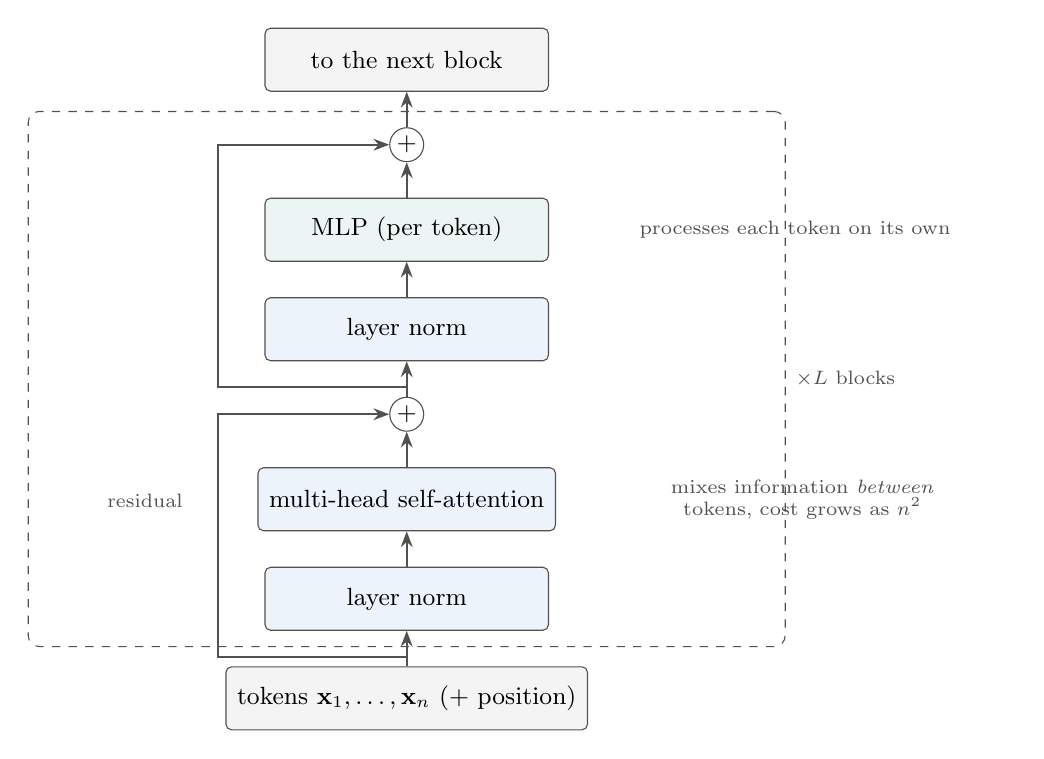
\begin{tikzpicture}[node distance=4.5mm, every node/.style={font=\small}]
\node[bx=gray, minimum width=3.6cm] (in) {tokens $\x_1,\dots,\x_n$ (+ position)};
\node[bx, above=of in, minimum width=3.6cm] (ln1) {layer norm};
\node[bx, above=of ln1, minimum width=3.6cm] (att) {multi-head self-attention};
\node[circle,draw=inkm,above=of att,inner sep=1pt] (p1) {$+$};
\node[bx, above=of p1, minimum width=3.6cm] (ln2) {layer norm};
\node[bx=cC, above=of ln2, minimum width=3.6cm] (mlp) {MLP (per token)};
\node[circle,draw=inkm,above=of mlp,inner sep=1pt] (p2) {$+$};
\node[bx=gray, above=of p2, minimum width=3.6cm] (out) {to the next block};
\draw[arr] (in)--(ln1); \draw[arr] (ln1)--(att); \draw[arr] (att)--(p1); \draw[arr] (p1)--(ln2); \draw[arr] (ln2)--(mlp); \draw[arr] (mlp)--(p2); \draw[arr] (p2)--(out);
\draw[arr] ($(in.north)+(0,0.12)$) -- ++(-2.4,0) |- (p1.west);
\draw[arr] ($(p1.north)+(0,0.12)$) -- ++(-2.4,0) |- (p2.west);
\node[lbl,anchor=east] at ($(p1.west)+(-2.5,-1.1)$) {residual};
\node[draw=inkm,dashed,rounded corners,fit=(ln1)(p2),inner xsep=30mm,inner ysep=2mm] (blk) {};
\node[lbl,anchor=west] at (blk.east) {$\times L$ blocks};
\node[lbl,anchor=west,text width=5.2cm] at ($(att.east)+(0.4,0)$) {mixes information \emph{between} tokens, cost grows as $n^2$};
\node[lbl,anchor=west,text width=5.2cm] at ($(mlp.east)+(0.4,0)$) {processes each token on its own};
\end{tikzpicture}
\caption{One transformer block (the ``pre-norm'' form used today). The residual paths carry the input around each sub-layer.}
\label{fig:block}
\end{figure}

\begin{watchbox}
Attention compares every token with every other token, so its cost grows with $n^2$. A camera image cut into 256 patches, a few frames of history and an instruction quickly give over a thousand tokens. This quadratic cost is one reason why VLAs run at only a few hertz, which matters for drones (Section~\ref{sec:dual}).
\end{watchbox}

\begin{quizbox}
\begin{enumerate}[leftmargin=*]
\item In the worked example, which token does ``cube'' attend to least, and why?
\item What would happen without a positional encoding to ``dog bites man'' and ``man bites dog''?
\item Why does a causal mask allow training on all positions at once?
\end{enumerate}
\emph{Answers: 1) ``the'', its key is short and points nowhere in particular; 2) each token gets exactly the same output in both sentences, so the model cannot tell who bites whom; 3) each position only sees its own past, so predicting token $t+1$ at every position $t$ is a valid training example and all of them are computed in one pass.}
\end{quizbox}

% --------------------------------------------------------------------
\section{Large language models, vision-language models and chain-of-thought}

\subsection{Next-token prediction}
A large language model (LLM) is a causal transformer trained on one task: given the tokens so far, predict the next one. The last layer outputs a score (logit) for each of the $V$ vocabulary tokens, the softmax turns them into probabilities, and the loss is the cross-entropy against the true next token. It is the course's multi-class classifier, applied trillions of times on internet text.

To generate, the model samples a token, appends it, and repeats. The \textbf{temperature} $T$ divides the logits before the softmax, $p_k\propto e^{\ell_k/T}$. Low $T$ makes the model nearly deterministic; high $T$ makes it more random (Figure~\ref{fig:temp}).

\begin{figure}[h]
\centering
\begin{tikzpicture}
\begin{axis}[ybar=1pt, bar width=6pt, width=9cm, height=4.6cm, ymin=0, ymax=0.9, xtick={0,1,2,3,4}, enlarge x limits=0.12,
  xticklabels={``cube'',``box'',``block'',``ball'',``cat''}, ylabel={probability}, legend pos=north east, xlabel={next token after ``pick up the red ...''}]
\addplot[fill=cA,draw=none] table[x=i,y=ta]{figs/temp.dat}; \addlegendentry{$T=0.5$}
\addplot[fill=cC,draw=none] table[x=i,y=tb]{figs/temp.dat}; \addlegendentry{$T=1$}
\addplot[fill=cB,draw=none] table[x=i,y=tc]{figs/temp.dat}; \addlegendentry{$T=2$}
\end{axis}
\end{tikzpicture}
\caption{The same logits $(3,\ 2.2,\ 1,\ 0.3,\ -0.5)$ at three temperatures. At $T=0.5$ ``cube'' gets 82\%; at $T=2$ only 40\%.}
\label{fig:temp}
\end{figure}

\begin{probbox}{the chain rule of probability: why next-token prediction models whole texts}
From the definition of conditional probability, $P(a,b)=P(a)\,P(b\mid a)$. Apply it again and again:
\[
p(x_1,x_2,\dots,x_n)=p(x_1)\,p(x_2\mid x_1)\,p(x_3\mid x_1,x_2)\cdots p(x_n\mid x_{<n})=\prod_{t=1}^n p(x_t\mid x_{<t}).
\]
This is exact; no assumption is made. Taking logs, $\log p(x_{1:n})=\sum_t\log p(x_t\mid x_{<t})$, so the next-token cross-entropy summed over a sequence \emph{is} the negative log-likelihood of the whole sequence. Generating one token at a time, each sampled from its conditional, produces exact samples of the joint distribution (``ancestral sampling''). The 7 action tokens of RT-2 or OpenVLA are generated the same way: $p(a^{(1)},\dots,a^{(7)})=\prod_i p(a^{(i)}\mid a^{(<i)},\text{obs})$.

\textbf{Check Figure~\ref{fig:temp} by hand.} At $T=1$: $e^{3}=20.09$, $e^{2.2}=9.03$, $e^{1}=2.72$, $e^{0.3}=1.35$, $e^{-0.5}=0.61$, sum $33.80$, so $p(\text{``cube''})=20.09/33.80=0.594$.
\end{probbox}

\subsection{From a text predictor to an assistant}
Training happens in stages, and the same stages reappear in robotics:
\begin{enumerate}
\item \textbf{Pre-training:} next-token prediction on huge unlabelled data. The model learns language, facts and some reasoning patterns.
\item \textbf{Supervised fine-tuning (SFT):} continue training on a smaller set of good examples (questions with ideal answers). This is imitation learning (Section~\ref{sec:il}) for text.
\item \textbf{Reinforcement learning:} let the model generate, score the result, and push up the probability of well-scored outputs. RLHF (Ouyang et al., 2022) uses a learned model of human preferences as the score. Newer reasoning models use \emph{verifiable rewards}, for example whether a maths answer is correct.
\end{enumerate}
\textbf{Fine-tuning cheaply.} Updating all billions of weights is expensive. \textbf{LoRA} (Hu et al., 2021) freezes them and learns a small low-rank correction $W+BA$ with $B\in\R^{d\times r}$, $A\in\R^{r\times d}$ and $r\approx 8$--$64$. This is how most people adapt an open VLA to their own robot on one or a few GPUs.

\subsection{Chain-of-thought and reasoning models}
\textbf{Chain-of-thought} (Wei et al., 2022) is the observation that an LLM answers multi-step questions much better if it first writes out intermediate steps. Each written step becomes part of the input for the next token, so the model gets extra computation and a scratchpad. \textbf{Reasoning models} (OpenAI o1 in 2024, DeepSeek-R1 in 2025) are trained with reinforcement learning to produce long chains of thought before answering; DeepSeek-R1 showed that rewarding only the correctness of the final answer is enough for useful reasoning behaviour to appear.

\begin{plainbox}
Chain-of-thought trades time for accuracy: more tokens before the answer means more computation spent on the problem. For a chatbot, a few extra seconds are fine. For a robot that must react within tens of milliseconds, they are a real cost. This tension is the central design problem of reasoning VLAs (Section~\ref{sec:rvla}).
\end{plainbox}

\subsection{Images as tokens: ViT and vision-language models}
The \textbf{vision transformer} (ViT, Dosovitskiy et al., 2021) cuts an image into patches, typically $16\times16$ pixels, flattens each patch, maps it to an embedding with a linear layer, adds a positional encoding, and feeds the patch tokens to a standard transformer. A $224\times224$ image becomes $14\times14=196$ tokens. Convolutions are no longer needed.

A \textbf{vision-language model} (VLM) connects such an image encoder to an LLM: the image tokens pass through a small projector (often an MLP) into the LLM's embedding space and are placed in front of the text tokens. The LLM then ``reads'' the image as if it were words. Examples are LLaVA (Liu et al., 2023) and PaliGemma (Google, 2024). Most VLAs are a VLM with an action output added (Figure~\ref{fig:vlm}).

\begin{figure}[h]
\centering
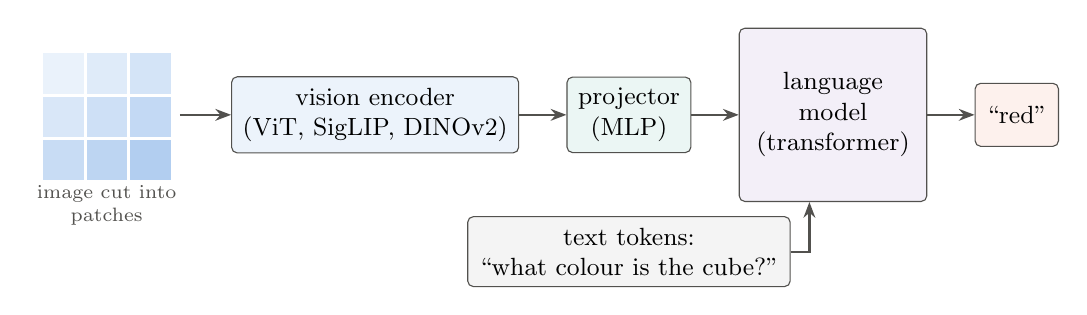
\begin{tikzpicture}[every node/.style={font=\small}]
\foreach \i in {0,1,2} \foreach \j in {0,1,2} \draw[fill=cA!\the\numexpr 10+8*\i+5*\j\relax, draw=white, line width=1pt] (\j*0.55,-\i*0.55) rectangle ++(0.55,-0.55);
\node[lbl] at (0.82,-1.95) {image cut into\\patches};
\node[bx=cA, anchor=west] (enc) at (2.4,-0.8) {vision encoder\\(ViT, SigLIP, DINOv2)};
\node[bx=cC, right=0.6cm of enc] (proj) {projector\\(MLP)};
\node[bx=cD, right=0.6cm of proj, minimum height=2.2cm, text width=2.1cm] (llm) {language model\\(transformer)};
\node[bx=gray, below=0.8cm of proj] (txt) {text tokens:\\``what colour is the cube?''};
\node[bx=cB, right=0.6cm of llm] (out) {``red''};
\draw[arr] (1.75,-0.8)--(enc); \draw[arr] (enc)--(proj); \draw[arr] (proj)--(llm.west|-proj); \draw[arr] (txt.east)-|([xshift=-3mm]llm.south); \draw[arr] (llm)--(out);
\end{tikzpicture}
\caption{A vision-language model. Image patches become tokens in the same space as words, and the language model processes both together.}
\label{fig:vlm}
\end{figure}

\begin{quizbox}
\begin{enumerate}[leftmargin=*]
\item Why is next-token prediction a classification problem?
\item What does LoRA train, and why is it cheap?
\item How many patch tokens does a $256\times256$ image give with $16\times16$ patches?
\end{enumerate}
\emph{Answers: 1) the target is one of $V$ discrete tokens; 2) two thin matrices $B$ and $A$ added to frozen weights, so only a tiny fraction of the parameters gets gradients and optimiser state; 3) $16\times16=256$.}
\end{quizbox}

% --------------------------------------------------------------------
\section{Generative models for continuous outputs: diffusion and flow matching}
\label{sec:diffusion}

\subsection{Why regression fails for actions}
Imagine a drone in front of a pole. Half of the human demonstrations fly left around it and half fly right. Train a regression model with squared error, and it predicts the \emph{mean} of the demonstrations: straight ahead, into the pole. The course's regression answer, $\E[y\mid\x]$, is the wrong answer when the data has several good modes. Figure~\ref{fig:bimodal} shows the toy version: the demonstrations cluster at $-1$ and $+1$, and the regression output is \bimean, between the modes, where no demonstration ever went.

\begin{figure}[h]
\centering
\begin{tikzpicture}
\begin{axis}[width=10cm,height=4.8cm, xmin=-2, xmax=2, ymin=0, ymax=1.65, xlabel={sideways action $a$ (left $<0<$ right)}, ylabel={density}, legend style={at={(0.5,1.03)},anchor=south}, legend columns=2]
\addplot[ybar interval, fill=cA!35, draw=cA!70] table[x=x,y=demo]{figs/bimodal.dat}; \addlegendentry{400 demonstrations}
\addplot[ybar interval, fill=none, draw=cB, thick] table[x=x,y=gen]{figs/bimodal.dat}; \addlegendentry{samples of a generative policy}
\draw[very thick, color=black] (axis cs:\bimean,0) -- (axis cs:\bimean,1.45) node[right,font=\scriptsize]{regression output};
\fill[gray!40] (axis cs:-0.25,0) rectangle (axis cs:0.25,0.12); \node[font=\scriptsize] at (axis cs:0,0.22) {pole};
\end{axis}
\end{tikzpicture}
\caption{Two equally good ways around an obstacle. Squared-error regression averages them and flies into the pole. A generative policy (here a two-component Gaussian mixture fitted to the same data) samples one mode or the other.}
\label{fig:bimodal}
\end{figure}

The fix is to learn the whole distribution $p(\av\mid\text{observation})$ and \emph{sample} from it. Three families appear in VLAs: discretise the action into tokens and use a softmax (which can represent several modes, Section~\ref{sec:actrep}); diffusion; and flow matching.

\begin{probbox}{the best guess under squared error is the mean; mixture distributions}
\textbf{Derivation.} Which single number $c$ minimises the expected squared error $f(c)=\E[(Y-c)^2]$? Expand: $f(c)=\E[Y^2]-2c\,\E[Y]+c^2$. Set the derivative to zero: $-2\E[Y]+2c=0$, so $c=\E[Y]$. With an input, the same argument for each $\x$ separately gives the best predictor $\hat y(\x)=\E[Y\mid\x]$, the \emph{conditional mean}. A network trained with MSE and enough data learns this conditional mean.

\textbf{Bias and variance again.} Adding and subtracting $\E Y$: $\E[(Y-c)^2]=\mathrm{Var}(Y)+(\E Y-c)^2$ (the cross term has expectation $2(\E Y-c)\E[Y-\E Y]=0$). The first part is noise no predictor can remove, the second is the error of the guess. This is the decomposition from your course book, for a single point.

\textbf{Why this is bad here.} Half the mass at $-1$ and half at $+1$ give $\E[Y]=\tfrac12(-1)+\tfrac12(+1)=0$: the pole. (The data in Figure~\ref{fig:bimodal} give \bimean.) Under absolute error the best guess is the \emph{median}, which for this data is also between the modes, so changing the loss does not help; changing the model does.

\textbf{Mixture distributions.} A Gaussian mixture is $p(a)=\sum_{k=1}^K\pi_k\,\mathcal N(a;\mu_k,\sigma_k^2)$ with weights $\pi_k\ge0$, $\sum_k\pi_k=1$. To sample: pick component $k$ with probability $\pi_k$, then sample from that Gaussian. The fit in Figure~\ref{fig:bimodal} found $\pi\approx(0.47,0.53)$, $\mu\approx(-1.03,\,0.98)$, $\sigma\approx0.17$. It was fitted with the EM algorithm, which alternates between computing, for each point, the probability that it came from each component, and refitting each component's mean and spread with those probabilities as weights.
\end{probbox}

\subsection{Diffusion: learn to remove noise}
Diffusion models (Ho et al., 2020) define a fixed process that slowly destroys data with Gaussian noise, and learn to run it backwards.
\begin{itemize}
\item \textbf{Forward (fixed):} $\x_t=\sqrt{\bar\alpha_t}\,\x_0+\sqrt{1-\bar\alpha_t}\,\bm\epsilon$ with $\bm\epsilon\sim\mathcal N(0,I)$, where $\bar\alpha_t$ falls from 1 (clean) to 0 (pure noise) as $t$ grows.
\item \textbf{Training:} a network $\bm\epsilon_\theta(\x_t,t)$ learns to predict the noise that was added: $\mathcal L=\E\lVert\bm\epsilon-\bm\epsilon_\theta(\x_t,t)\rVert^2$. This is ordinary regression with a squared error.
\item \textbf{Sampling:} start from pure noise and repeatedly subtract a little of the predicted noise, typically 10--100 steps.
\end{itemize}
The regression here does not average modes away, because the network only predicts the \emph{noise} at each step, and early noisy steps decide which mode the sample falls into. Figure~\ref{fig:diff} shows the distribution of our bimodal action at four noise levels, computed in closed form.

\begin{figure}[h]
\centering
\begin{tikzpicture}
\begin{axis}[width=10cm,height=4.8cm, xmin=-3, xmax=3, ymin=0, ymax=1.5, xlabel={action $x$}, ylabel={density $p(x_t)$}, legend pos=north east]
\addplot[very thick, cA] table[x=x,y=p0]{figs/diffusion.dat}; \addlegendentry{$\bar\alpha=1$ (data)}
\addplot[thick, cC] table[x=x,y=p1]{figs/diffusion.dat}; \addlegendentry{$\bar\alpha=0.7$}
\addplot[thick, cD] table[x=x,y=p2]{figs/diffusion.dat}; \addlegendentry{$\bar\alpha=0.3$}
\addplot[thick, dashed, cB] table[x=x,y=p3]{figs/diffusion.dat}; \addlegendentry{$\bar\alpha=0$ (noise)}
\end{axis}
\end{tikzpicture}
\caption{The forward diffusion process on the bimodal action data. Noise blurs the two peaks into a single Gaussian. Sampling runs this picture from the dashed curve back to the blue one.}
\label{fig:diff}
\end{figure}

\begin{probbox}{scaling and adding Gaussians; the curves of Figure~\ref{fig:diff}}
\textbf{Rule.} If $X\sim\mathcal N(m,v)$ and $\epsilon\sim\mathcal N(0,1)$ are independent, then $aX+b\epsilon\sim\mathcal N(am,\ a^2v+b^2)$. The mean follows from linearity of expectation, the variance from $\mathrm{Var}(aX)=a^2\mathrm{Var}(X)$ plus ``variances of independent variables add''; that the result is again Gaussian is a special property of the Gaussian.

\textbf{Why the square roots.} With $a=\sqrt{\bar\alpha_t}$ and $b=\sqrt{1-\bar\alpha_t}$: if the data has variance 1, then $\mathrm{Var}(\x_t)=\bar\alpha_t\cdot1+(1-\bar\alpha_t)=1$ at every step. The noise replaces the signal without changing the overall scale (``variance preserving'').

\textbf{The curves.} Our data is the mixture $\tfrac12\mathcal N(-1,s_0^2)+\tfrac12\mathcal N(+1,s_0^2)$ with $s_0=0.15$. Applying the rule to each component:
\[
p(x_t)=\tfrac12\,\mathcal N\big(x;-\sqrt{\bar\alpha},\ \bar\alpha s_0^2+1-\bar\alpha\big)+\tfrac12\,\mathcal N\big(x;+\sqrt{\bar\alpha},\ \bar\alpha s_0^2+1-\bar\alpha\big).
\]
At $\bar\alpha=1$ this is the data; at $\bar\alpha=0$ both components become $\mathcal N(0,1)$. These are exactly the four curves plotted.

\textbf{Why predicting the noise is enough.} Given $\x_t$ and a noise estimate $\hat{\bm\epsilon}$, invert the forward formula: $\hat\x_0=(\x_t-\sqrt{1-\bar\alpha_t}\,\hat{\bm\epsilon})/\sqrt{\bar\alpha_t}$. By the previous box, the network trained with squared error learns $\E[\bm\epsilon\mid\x_t]$. When $\x_t$ is only slightly noisy it already reveals which mode it came from, so this average is taken within one mode, and the modes are not averaged together.
\end{probbox}

\subsection{Flow matching: learn a velocity field}
Flow matching (Lipman et al., 2023) is a simpler relative that is now the standard in VLAs (it is what $\pi_0$ uses). Pair a noise sample $\x_0\sim\mathcal N(0,I)$ with a data sample $\x_1$, and connect them by a straight line $\x_\tau=(1-\tau)\x_0+\tau\x_1$ for $\tau\in[0,1]$. The velocity along that line is $\x_1-\x_0$. A network $\vect v_\theta(\x_\tau,\tau)$ learns to predict it:
\begin{equation}
\mathcal L=\E_{\tau,\x_0,\x_1}\big\lVert \vect v_\theta(\x_\tau,\tau)-(\x_1-\x_0)\big\rVert^2 .
\end{equation}
To sample, start from noise and integrate $\mathrm d\x/\mathrm d\tau=\vect v_\theta(\x,\tau)$ from $\tau=0$ to $1$ with a few Euler steps (often 5--10). In a robot the network is also given the observation, so it learns $p(\av\mid\text{obs})$.

\begin{figure}[h]
\centering
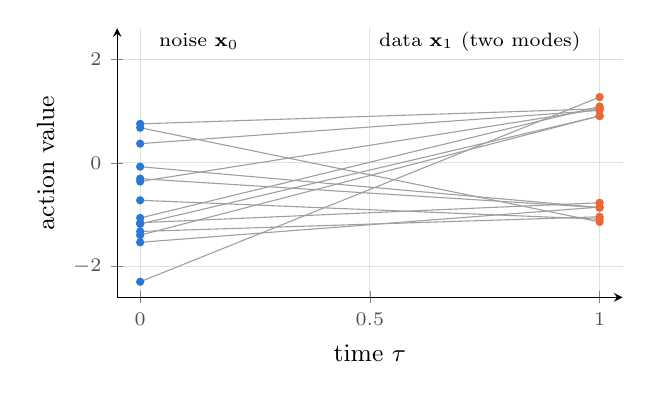
\begin{tikzpicture}
\begin{axis}[width=8cm,height=5cm, xmin=-0.05, xmax=1.05, ymin=-2.6, ymax=2.6, xlabel={time $\tau$}, ylabel={action value}, xtick={0,0.5,1}]
\draw[flowp] (axis cs:0,-0.724) -- (axis cs:1,-1.089);
\fill[cA] (axis cs:0,-0.724) circle (1.5pt);
\fill[cB] (axis cs:1,-1.089) circle (1.5pt);
\draw[flowp] (axis cs:0,-0.306) -- (axis cs:1,-0.865);
\fill[cA] (axis cs:0,-0.306) circle (1.5pt);
\fill[cB] (axis cs:1,-0.865) circle (1.5pt);
\draw[flowp] (axis cs:0,-1.398) -- (axis cs:1,0.908);
\fill[cA] (axis cs:0,-1.398) circle (1.5pt);
\fill[cB] (axis cs:1,0.908) circle (1.5pt);
\draw[flowp] (axis cs:0,-1.326) -- (axis cs:1,-1.043);
\fill[cA] (axis cs:0,-1.326) circle (1.5pt);
\fill[cB] (axis cs:1,-1.043) circle (1.5pt);
\draw[flowp] (axis cs:0,-1.157) -- (axis cs:1,-0.772);
\fill[cA] (axis cs:0,-1.157) circle (1.5pt);
\fill[cB] (axis cs:1,-0.772) circle (1.5pt);
\draw[flowp] (axis cs:0,-0.361) -- (axis cs:1,1.038);
\fill[cA] (axis cs:0,-0.361) circle (1.5pt);
\fill[cB] (axis cs:1,1.038) circle (1.5pt);
\draw[flowp] (axis cs:0,0.370) -- (axis cs:1,1.013);
\fill[cA] (axis cs:0,0.370) circle (1.5pt);
\fill[cB] (axis cs:1,1.013) circle (1.5pt);
\draw[flowp] (axis cs:0,-2.298) -- (axis cs:1,1.269);
\fill[cA] (axis cs:0,-2.298) circle (1.5pt);
\fill[cB] (axis cs:1,1.269) circle (1.5pt);
\draw[flowp] (axis cs:0,0.752) -- (axis cs:1,1.043);
\fill[cA] (axis cs:0,0.752) circle (1.5pt);
\fill[cB] (axis cs:1,1.043) circle (1.5pt);
\draw[flowp] (axis cs:0,-1.182) -- (axis cs:1,0.902);
\fill[cA] (axis cs:0,-1.182) circle (1.5pt);
\fill[cB] (axis cs:1,0.902) circle (1.5pt);
\draw[flowp] (axis cs:0,-1.066) -- (axis cs:1,1.088);
\fill[cA] (axis cs:0,-1.066) circle (1.5pt);
\fill[cB] (axis cs:1,1.088) circle (1.5pt);
\draw[flowp] (axis cs:0,0.678) -- (axis cs:1,-1.142);
\fill[cA] (axis cs:0,0.678) circle (1.5pt);
\fill[cB] (axis cs:1,-1.142) circle (1.5pt);
\draw[flowp] (axis cs:0,-0.075) -- (axis cs:1,-0.865);
\fill[cA] (axis cs:0,-0.075) circle (1.5pt);
\fill[cB] (axis cs:1,-0.865) circle (1.5pt);
\draw[flowp] (axis cs:0,-1.536) -- (axis cs:1,-0.855);
\fill[cA] (axis cs:0,-1.536) circle (1.5pt);
\fill[cB] (axis cs:1,-0.855) circle (1.5pt);

\node[font=\scriptsize,anchor=west] at (axis cs:0.02,2.35) {noise $\x_0$};
\node[font=\scriptsize,anchor=east] at (axis cs:0.98,2.35) {data $\x_1$ (two modes)};
\end{axis}
\end{tikzpicture}
\caption{Flow-matching training pairs. Each grey line connects a noise sample (blue) to a data sample (orange). The network learns the average velocity of the lines passing through each point, and integrating that velocity carries noise to data.}
\label{fig:flow}
\end{figure}

\begin{probbox}{why regressing on single pairs gives the right velocity field}
Many grey lines in Figure~\ref{fig:flow} pass through the same point $(\tau,x)$, each with its own target velocity $u=x_1-x_0$. The network cannot match all of them. By the ``best guess is the mean'' box, the minimiser of $\E\lVert\vect v(\x_\tau,\tau)-\vect u\rVert^2$ is the conditional mean
\[
\vect v^\star(\x,\tau)=\E\big[\x_1-\x_0\ \big|\ \x_\tau=\x\big],
\]
the average velocity of all lines through that point. Lipman et al.\ (2023) proved that following this averaged field from $\tau=0$ to $1$ carries the noise distribution exactly onto the data distribution, even though no single sample moves along a straight line any more. Sampling uses Euler steps, $\x_{\tau+\Delta}=\x_\tau+\Delta\,\vect v_\theta(\x_\tau,\tau)$; with $\Delta=0.1$ that is ten network calls.
\end{probbox}

\begin{plainbox}
Diffusion and flow matching turn ``generate a sample from a complicated distribution'' into many small regression problems. That is why they train as stably as regression but do not average modes away. The price is several network evaluations per sample instead of one.
\end{plainbox}

\begin{quizbox}
\begin{enumerate}[leftmargin=*]
\item Give a drone example of a bimodal action distribution other than the pole.
\item In flow matching, what is the regression target for the pair $\x_0=-0.5$, $\x_1=1$?
\item Why do diffusion and flow models need several network calls per sample?
\end{enumerate}
\emph{Answers: 1) e.g.\ overtaking another drone above or below it, or entering a room through either of two doors; 2) the velocity $1-(-0.5)=1.5$, at every $\tau$; 3) a sample is produced by integrating many small steps from noise to data.}
\end{quizbox}

\part{Robot-learning background}
% ============================== PART II ==============================
\section{Decisions over time: MDPs and reinforcement learning}
\label{sec:rl}

\subsection{The language of sequential decisions}
Classification makes one decision. A robot makes a decision every few milliseconds, and each one changes what it will see next. The standard model is the \textbf{Markov decision process} (MDP):
\begin{itemize}
\item a state $s_t$ (for a drone: position, velocity, attitude, the obstacles around it);
\item an action $a_t$ (thrust and body rates, or a velocity command);
\item dynamics $p(s_{t+1}\mid s_t,a_t)$: what happens next;
\item a reward $r_t=r(s_t,a_t)$: how good that step was;
\item a policy $\pi(a_t\mid s_t)$: the controller, which is what we want to learn.
\end{itemize}
The goal is to maximise the expected \textbf{return} $G=\sum_{t\ge0}\gamma^t r_t$, where the discount $\gamma\in(0,1)$ (say $0.99$) makes near rewards count more than far ones. ``Markov'' means $s_t$ contains everything needed to predict the future; the past adds nothing.

\begin{probbox}{the Markov property, expected return and the geometric series}
\textbf{Markov property, as a formula:} $p(s_{t+1}\mid s_t,a_t,s_{t-1},a_{t-1},\dots,s_0)=p(s_{t+1}\mid s_t,a_t)$.

\textbf{Why an expectation.} The dynamics and usually the policy are random, so the return $G$ is a random variable. We maximise its expectation $\E[G]$, the average return over many runs.

\textbf{Why the return is finite.} If every reward satisfies $|r_t|\le r_{\max}$, then $|G|\le r_{\max}\sum_{t\ge0}\gamma^t$. The geometric series: let $S=1+\gamma+\gamma^2+\dots$; then $\gamma S=\gamma+\gamma^2+\dots$, and subtracting, $S-\gamma S=1$, so $S=\dfrac{1}{1-\gamma}$ for $0\le\gamma<1$. Hence $|G|\le r_{\max}/(1-\gamma)$. With $\gamma=0.99$ the sum is 100: the discount makes the agent look roughly 100 steps ahead.
\end{probbox}

A real robot does not see the state. It sees an \textbf{observation} $o_t$, such as a camera image, which is only part of the state. This is a \emph{partially observable} MDP (POMDP). The usual fix is to keep a memory, a hidden state $\h_t$ built from all past observations and actions. Keep this in mind: the hidden state of a world model (Section~\ref{sec:dreamer}) is exactly this memory.

\begin{figure}[h]
\centering
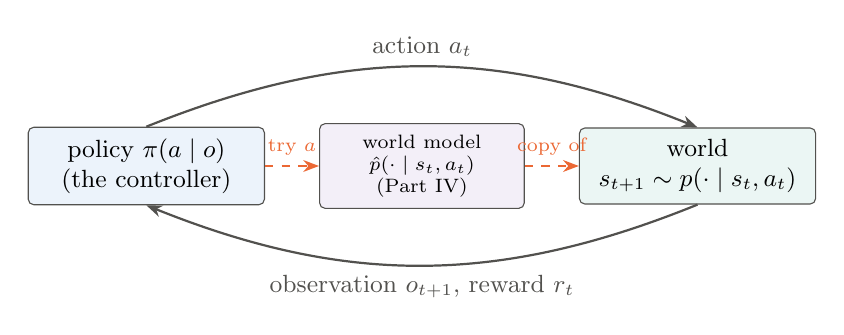
\begin{tikzpicture}[every node/.style={font=\small}]
\node[bx=cA, minimum width=3cm] (ag) at (0,0) {policy $\pi(a\mid o)$\\(the controller)};
\node[bx=cC, minimum width=3cm] (env) at (7,0) {world\\$s_{t+1}\sim p(\cdot\mid s_t,a_t)$};
\draw[arr] (ag.north) to[bend left=22] node[above]{action $a_t$} (env.north);
\draw[arr] (env.south) to[bend left=22] node[below]{observation $o_{t+1}$, reward $r_t$} (ag.south);
\node[bx=cD, minimum width=2.6cm, font=\scriptsize] (wm) at (3.5,0) {world model\\$\hat p(\cdot\mid s_t,a_t)$\\(Part IV)};
\draw[darr] (ag.east)--(wm.west) node[midway,above,font=\scriptsize]{try $a$};
\draw[darr] (wm.east)--(env.west) node[midway,above,font=\scriptsize]{copy of};
\end{tikzpicture}
\caption{The agent--environment loop from the course's reinforcement-learning section. A world model (dashed) is a learned copy of the right-hand box that the agent can query without moving.}
\label{fig:loop}
\end{figure}

\begin{bridgebox}
Course book, the reinforcement-learning loop in Part I. There, RL was ``learn from rewards by trial and error''. Here we add the pieces needed to read papers: states versus observations, the discount, value functions, and the split into model-free and model-based methods.
\end{bridgebox}

\subsection{Values and policy gradients in one page}
The \textbf{value} $V^\pi(s)$ is the expected return from state $s$ when following $\pi$. The \textbf{action value} $Q^\pi(s,a)$ is the same, but taking action $a$ first. They satisfy the Bellman equation
\begin{equation}
Q^\pi(s,a)=r(s,a)+\gamma\,\E_{s'\sim p(\cdot\mid s,a)}\big[V^\pi(s')\big],\label{eq:bellman}
\end{equation}
which says: value now $=$ reward now $+$ discounted value of where you land. A neural network trained to satisfy this equation is a \emph{critic}.

\begin{probbox}{deriving the Bellman equation}
\textbf{Step 1: the return is recursive.} $G_t=r_t+\gamma r_{t+1}+\gamma^2r_{t+2}+\dots=r_t+\gamma\,(r_{t+1}+\gamma r_{t+2}+\dots)=r_t+\gamma G_{t+1}$.

\textbf{Step 2: take expectations.} By definition $Q^\pi(s,a)=\E[G_t\mid s_t=s,a_t=a]$. By linearity,
\[
Q^\pi(s,a)=r(s,a)+\gamma\,\E[G_{t+1}\mid s_t=s,a_t=a].
\]
\textbf{Step 3: the law of total expectation}, $\E[X]=\E_Y\big[\E[X\mid Y]\big]$ (average within each case of $Y$, then average over the cases). Condition on the next state $s'$:
\[
\E[G_{t+1}\mid s,a]=\E_{s'\sim p(\cdot\mid s,a)}\big[\E[G_{t+1}\mid s_{t+1}=s']\big]=\E_{s'}\big[V^\pi(s')\big].
\]
The Markov property lets us drop $s,a$ inside the inner expectation: once $s'$ is known, the earlier state adds nothing. Substituting gives equation~\eqref{eq:bellman}.
\end{probbox}

A \textbf{policy gradient} method changes the policy directly. Its core formula is
\begin{equation}
\nabla_\theta J=\E\big[\nabla_\theta\log\pi_\theta(a_t\mid s_t)\,A_t\big],\qquad A_t=Q(s_t,a_t)-V(s_t),
\end{equation}
where the \emph{advantage} $A_t$ says whether the action was better or worse than usual. In words: make better-than-usual actions more likely and worse-than-usual actions less likely. PPO (Schulman et al., 2017) is the most used version; it limits how far each update can move the policy. An \textbf{actor--critic} method trains a policy (actor) and a value network (critic) together. Dreamer does exactly this, but inside its world model.

\begin{probbox}{deriving the policy gradient (the log-derivative trick)}
We want $\nabla_\theta\E_{a\sim\pi_\theta}[f(a)]$, the gradient of an average whose \emph{distribution} depends on $\theta$. Write it as a sum and use $\nabla\pi=\pi\,\nabla\log\pi$ (because $\nabla\log\pi=\nabla\pi/\pi$):
\[
\nabla_\theta\sum_a\pi_\theta(a)f(a)=\sum_a\nabla_\theta\pi_\theta(a)\,f(a)=\sum_a\pi_\theta(a)\,\nabla_\theta\log\pi_\theta(a)\,f(a)=\E_{a\sim\pi_\theta}\big[f(a)\,\nabla_\theta\log\pi_\theta(a)\big].
\]
The right side is an expectation again, so it can be estimated from sampled actions without knowing how $f$ (the environment) works. For whole trajectories, the probability is a product of policy terms and dynamics terms; the log turns it into a sum, and the dynamics terms vanish from the gradient because they do not depend on $\theta$.

\textbf{Why subtracting a baseline is allowed.} For any $b$ that does not depend on the action,
$\E[b\,\nabla\log\pi]=b\sum_a\nabla\pi(a)=b\,\nabla\sum_a\pi(a)=b\,\nabla1=0$. So replacing $f$ by $f-V(s)$, the advantage, does not change the expected gradient, but it makes the estimate much less noisy.
\end{probbox}

\subsection{Model-free and model-based RL}
\begin{itemize}
\item \textbf{Model-free} RL (PPO, SAC) learns the policy from real or simulated experience and never learns the dynamics. It is simple and robust, but needs millions of steps. That is fine in a fast simulator and impossible on a real drone.
\item \textbf{Model-based} RL first learns the dynamics $\hat p(s'\mid s,a)$, a world model, and then plans with it or trains the policy on imagined experience. It needs far less real data. It is only as good as the model, and model errors compound over long horizons (Section~\ref{sec:compound}).
\end{itemize}

\subsection{Simulation, sim-to-real and a drone landmark}
Most robot RL trains in simulation and then transfers to the real robot. The gap between the two (wrong mass, motor delays, camera noise, aerodynamic effects) is the \textbf{sim-to-real gap}. The standard tool against it is \textbf{domain randomisation}: train on many simulators with randomised masses, delays and textures, so that the real world looks like one more variation.

\begin{paperbox}{Kaufmann et al.\ (2023), ``Champion-level drone racing using deep reinforcement learning'', Nature}
The \emph{Swift} system beat human world champions in first-person-view drone racing. The policy was trained with model-free RL (PPO) in simulation. Its observations came from onboard vision and inertial sensing. To close the sim-to-real gap, the authors fitted small \emph{residual models} of perception and dynamics from real flight data and added them to the simulator. Lesson for you: on drones, learned control works best when the learning happens in simulation and a small amount of real data is used to correct the simulator, which is a modest form of world model.
\end{paperbox}

\begin{quizbox}
\begin{enumerate}[leftmargin=*]
\item Why is a single camera image not a Markov state for a drone?
\item With $\gamma=0.9$, how much is a reward of 1 worth if it arrives 10 steps from now?
\item Why can't you run PPO directly on a tiny whoop?
\end{enumerate}
\emph{Answers: 1) one frame shows position but not velocity, and things outside the view are missing; 2) $0.9^{10}\approx0.35$; 3) it needs millions of trials, most of which would be crashes.}
\end{quizbox}

% --------------------------------------------------------------------
\section{Imitation learning: learning from demonstrations}
\label{sec:il}

\subsection{Behaviour cloning}
Rewards are hard to write for ``fold the towel'' or ``fly through the doorway and land on the table''. It is often easier to \emph{show} the robot. A human teleoperates it many times, and we record pairs (observation, action). \textbf{Behaviour cloning} (BC) then fits a policy by supervised learning:
\begin{equation}
\pi_\theta=\argmin_\theta\ \frac1N\sum_n -\log\pi_\theta(a_n\mid o_n).
\end{equation}
This is the course's regression or classification, with the observation as input and the action as label. Every VLA in Part III is trained mainly this way.

\subsection{The catch: covariate shift}
In the course, training and test data come from the same distribution. In BC they do not. The policy is trained on states the \emph{expert} visited, but at test time it visits states produced by \emph{its own} actions. A small mistake moves it into a state the expert never showed; there it makes a bigger mistake, and so on. Ross and Bagnell (2010) showed that if the policy errs with probability $\epsilon$ per step, the expected cost over a task of length $T$ can grow like $\epsilon T^2$, instead of the $\epsilon T$ you would expect from independent mistakes.

\begin{probbox}{distribution shift, and where $\epsilon T^2$ comes from}
\textbf{Covariate shift} means the distribution of inputs changes between training and test while the correct input--output rule stays the same. Behaviour cloning minimises $\E_{s\sim d_{\text{expert}}}[\ell(s)]$, but the cost we care about is $\E_{s\sim d_{\pi}}[\ell(s)]$, where $d_\pi$ is the distribution of states the learner itself visits.

\textbf{Worst-case argument.} Suppose the learner makes a mistake with probability at most $\epsilon$ in any state the expert visits, and that after its first mistake it is lost and pays cost 1 at every remaining step. The probability that the first mistake happens at step $t$ is at most $\epsilon$ (union bound), and it then pays at most $T-t+1$. So
\[
\E[\text{cost}]\ \le\ \sum_{t=1}^{T}\epsilon\,(T-t+1)=\epsilon\,\frac{T(T+1)}{2}\approx\frac{\epsilon T^2}{2}.
\]
If mistakes did not push the learner off its data, each step would independently cost $\epsilon$ in expectation, $\epsilon T$ in total. DAgger trains on $d_\pi$ itself, which brings the cost back to order $\epsilon T$. Ross and Bagnell also show that the quadratic bound can actually be reached.
\end{probbox}

Figure~\ref{fig:covshift} shows this on a toy lane-keeping task, $x_{t+1}=x_t+a_t+\text{noise}$. The expert steers with $a=-0.6x$ and stays in a narrow band around the centre (shaded, from $\bandlo$ to $\bandhi$). A degree-5 polynomial fitted to the expert's data is excellent \emph{inside} the band. At $t=10$ a gust pushes the car out of the band. The cloned policy has never seen such a state; its polynomial extrapolates wildly and the car ends at the edge of the road ($x=\pm3$, the clip). The expert recovers at once.

\begin{figure}[h]
\centering
\begin{tikzpicture}
\begin{axis}[width=11cm,height=5.4cm, xmin=0, xmax=40, ymin=-3.2, ymax=3.2, xlabel={time step $t$}, ylabel={lateral position $x$}, legend pos=north east, legend columns=3]
\fill[cA!30] (axis cs:0,\bandlo) rectangle (axis cs:40,\bandhi);
\addplot[cB, thick] table[x=t,y=b0]{figs/covshift.dat}; \addlegendentry{behaviour cloning}
\addplot[cC, thick] table[x=t,y=d0]{figs/covshift.dat}; \addlegendentry{after DAgger}
\addplot[black, dashed, thick] table[x=t,y=e]{figs/covshift.dat}; \addlegendentry{expert}
\addplot[cB, thick, forget plot] table[x=t,y=b1]{figs/covshift.dat};
\addplot[cB, thick, forget plot] table[x=t,y=b2]{figs/covshift.dat};
\addplot[cB, thick, forget plot] table[x=t,y=b3]{figs/covshift.dat};
\addplot[cC, thick, forget plot] table[x=t,y=d1]{figs/covshift.dat};
\addplot[cC, thick, forget plot] table[x=t,y=d2]{figs/covshift.dat};
\addplot[cC, thick, forget plot] table[x=t,y=d3]{figs/covshift.dat};
\draw[arr] (axis cs:10,1.6) -- (axis cs:10,0.8) node[pos=0,above,font=\scriptsize]{gust};
\end{axis}
\end{tikzpicture}
\caption{Covariate shift in a toy lane-keeping task (four rollouts each). The shaded band is where the expert's training data lies. After the gust, the cloned policy is outside its data and diverges; the DAgger policy, trained on states the learner itself visited, recovers.}
\label{fig:covshift}
\end{figure}

\subsection{Three fixes}
\begin{enumerate}
\item \textbf{DAgger} (Ross, Gordon \& Bagnell, 2011): let the learner drive, ask the expert what it \emph{would} have done in the states the learner visited, add these labels to the data, retrain, repeat. This fixes the distribution mismatch and brings the error back to linear in $T$. In Figure~\ref{fig:covshift}, five DAgger rounds were enough. The price is that the expert must be available during training.
\item \textbf{More diverse data:} include recoveries and disturbances in the demonstrations. Large robot datasets do this implicitly by covering many situations.
\item \textbf{Action chunking:} predict several future actions at once (next subsection). Fewer decisions per task means fewer chances to drift.
\end{enumerate}

\subsection{Action chunking and modern BC policies}
\textbf{ACT} (Zhao et al., 2023, with the ALOHA robot) predicts a \emph{chunk} of the next $k$ actions from one observation, for example $k=100$ steps of joint targets at 50~Hz. The task horizon in ``decisions'' shrinks by a factor $k$, and the chunks give smooth motion. Overlapping chunks are averaged (temporal ensembling). \textbf{Diffusion Policy} (Chi et al., 2023) combines chunking with a diffusion model over the chunk, which handles multimodal demonstrations (Section~\ref{sec:diffusion}). Almost every VLA after 2024 outputs action chunks.

\begin{figure}[h]
\centering
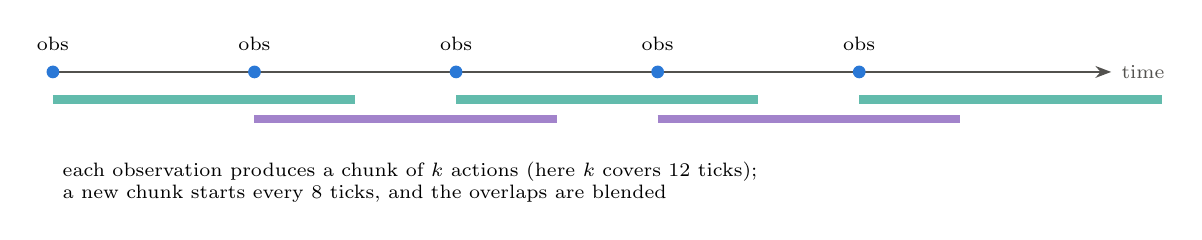
\begin{tikzpicture}[x=0.32cm,every node/.style={font=\scriptsize}]
\draw[arr] (0,0)--(42,0) node[right]{time};
\foreach \t in {0,8,16,24,32} {\fill[cA] (\t,0) circle (2.3pt); \node[above] at (\t,0.15) {obs};}
\foreach \t/\c in {0/cC,8/cD,16/cC,24/cD,32/cC} {\draw[\c, line width=3pt, opacity=0.7] (\t,{-0.35-0.25*mod(\t/8,2)}) -- ++(12,0);}
\node[anchor=west, align=left] at (0,-1.4) {each observation produces a chunk of $k$ actions (here $k$ covers 12 ticks);\\a new chunk starts every 8 ticks, and the overlaps are blended};
\end{tikzpicture}
\caption{Action chunking. The policy is queried at a slow rate, but every query fills a buffer of future actions that a fast loop plays back.}
\label{fig:chunk}
\end{figure}

\subsection{Robot data}
Robot data is expensive: someone has to teleoperate a real robot. The largest open collections are \textbf{Open X-Embodiment} (2023; more than a million trajectories from over twenty robot types, pooled by many labs) and \textbf{DROID} (2024; about 76\,000 teleoperated trajectories with one arm in hundreds of real scenes). By internet standards this is tiny. That shortage is why VLAs start from a VLM pretrained on web images and text, and why world models that can learn from ordinary \emph{video without actions} are so attractive.

\begin{quizbox}
\begin{enumerate}[leftmargin=*]
\item In your own words: why does the cloned policy in Figure~\ref{fig:covshift} fail even though its training error is tiny?
\item What does DAgger need that plain BC does not?
\item If a policy outputs chunks of 50 actions at 50~Hz, how often must the network run?
\end{enumerate}
\emph{Answers: 1) its training data covers only the narrow band, and after the gust it is evaluated far outside it, which is extrapolation; 2) an expert who can label new states on demand; 3) at least once per second, and in practice more often (e.g.\ every 0.2--0.5~s) so that it can react.}
\end{quizbox}

\part{Vision-language-action models}
% ============================== PART III ==============================
\section{Vision-language-action models}
\label{sec:vla}

\subsection{What a VLA is}
A vision-language-action model is a policy
\begin{equation}
\pi_\theta\big(\,a_{t:t+k}\ \big|\ \text{images}_t,\ \text{instruction},\ \text{robot state}_t\big),
\end{equation}
built by taking a pretrained vision-language model (Figure~\ref{fig:vlm}) and teaching it to output an action chunk instead of, or in addition to, text. It is trained by behaviour cloning (Section~\ref{sec:il}) on robot demonstrations, usually mixed with some of the original web data so that it keeps its general knowledge. The hope is that the VLM's knowledge of objects, words and scenes transfers: a robot that was never shown a ``dinosaur toy'' can still pick one up, because the VLM knows what a dinosaur looks like.

\subsection{Three ways to output actions}
\label{sec:actrep}
\textbf{1.\ Actions as tokens (RT-1, RT-2, OpenVLA).} Clip each action dimension to its range and cut the range into 256 equal bins. Each bin becomes a token, and the language model predicts the action tokens one after another with its normal softmax, exactly like words. RT-2 and OpenVLA reuse 256 rarely used tokens of the vocabulary for this.

\begin{examplebox}
An end-effector velocity in $[-1,1]$~m/s with 256 bins gives a bin width of $2/256\approx0.0078$~m/s. The value $0.30$ falls into bin $\lfloor (0.30+1)/2\cdot256\rfloor=\lfloor166.4\rfloor=166$. Decoding takes the bin centre, $-1+(166+0.5)\cdot 2/256\approx0.3008$~m/s, so the rounding error is under 1~mm/s. A 7-dimensional arm action (3 position, 3 rotation, 1 gripper) is 7 tokens, generated one by one.
\end{examplebox}

\begin{probbox}{the rounding error of action bins: the uniform distribution}
If the true value is equally likely to be anywhere inside its bin of width $\Delta$, the rounding error $e$ is \textbf{uniform} on $[-\Delta/2,\Delta/2]$, with density $1/\Delta$ there. Its mean is 0 by symmetry, and its variance is
\[
\mathrm{Var}(e)=\int_{-\Delta/2}^{\Delta/2}e^2\,\frac{1}{\Delta}\,\mathrm de=\frac1\Delta\Big[\frac{e^3}{3}\Big]_{-\Delta/2}^{\Delta/2}=\frac1\Delta\cdot\frac{2}{3}\cdot\frac{\Delta^3}{8}=\frac{\Delta^2}{12}.
\]
So the typical (root-mean-square) error is $\Delta/\sqrt{12}\approx0.29\,\Delta$. For $\Delta=0.0078$~m/s that is about $0.0023$~m/s, and the worst case is $\Delta/2\approx0.0039$~m/s.
\end{probbox}

\begin{figure}[h]
\centering
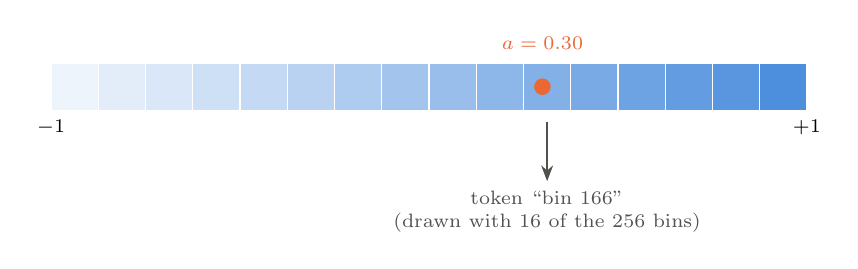
\begin{tikzpicture}[x=0.6cm,every node/.style={font=\scriptsize}]
\foreach \i in {0,...,15} \draw[draw=white,fill=cA!\the\numexpr 8+5*\i\relax] (\i,0) rectangle ++(1,0.6);
\fill[cB] (10.4,0.3) circle (3pt);
\node[below] at (0,0) {$-1$}; \node[below] at (16,0) {$+1$};
\node[above,color=cB] at (10.4,0.65) {$a=0.30$};
\draw[arr] (10.5,-0.15) -- (10.5,-0.9) node[below,align=center]{token ``bin 166''\\(drawn with 16 of the 256 bins)};
\end{tikzpicture}
\caption{Action tokenisation: a continuous value becomes the index of its bin, which the language model predicts like a word.}
\end{figure}

Tokens are simple and reuse the language model unchanged, and the softmax can represent several modes. They are slow (one network pass per token, and seven or more tokens per time step), and they are coarse for very precise or high-frequency control.

\textbf{2.\ Compressed action tokens (FAST, Pertsch et al., 2025).} Take a whole chunk of actions, apply a discrete cosine transform (the same transform JPEG uses for images), keep the important coefficients, and compress them with byte-pair encoding. A smooth one-second chunk becomes a few dozen tokens instead of hundreds, which makes token-based VLAs much faster to train on high-frequency data.

\textbf{3.\ A continuous action expert ($\pi_0$, GR00T N1).} Keep the VLM for understanding, and add a separate, smaller transformer, the \emph{action expert}, that produces a continuous action chunk with flow matching or diffusion (Section~\ref{sec:diffusion}). The action expert attends to the VLM's internal tokens. This is the dominant design in 2025--2026.

\subsection{One forward pass, step by step}
Figure~\ref{fig:pi0} follows a $\pi_0$-style model through one control step.
\begin{enumerate}
\item Each camera image ($224\times224$) is cut into patches and encoded into a few hundred tokens by the vision encoder.
\item The instruction ``put the red cube in the box'' becomes about ten text tokens.
\item The VLM processes images and text together and produces a sequence of internal feature vectors.
\item The action expert receives the robot's joint state, a chunk of 50 \emph{noisy} actions and the flow time $\tau$. Its tokens attend to the VLM features.
\item It predicts the velocity field; ten Euler steps turn noise into a clean chunk of 50 actions.
\item A low-level controller executes the chunk while the next one is being computed.
\end{enumerate}

\begin{figure}[h]
\centering
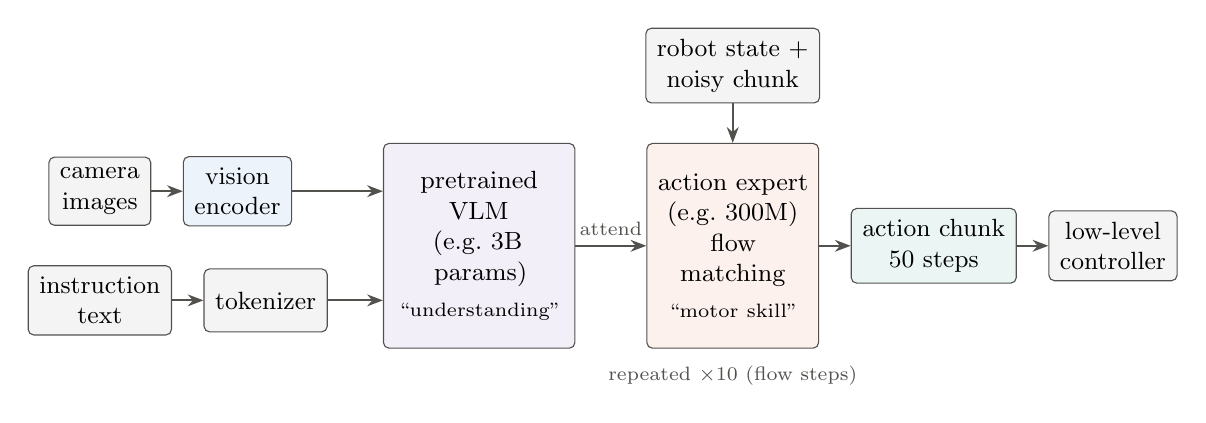
\begin{tikzpicture}[node distance=5mm and 4mm, every node/.style={font=\footnotesize}]
\node[bx=gray] (img) {camera\\images};
\node[bx=gray, below=of img] (txt) {instruction\\text};
\node[bx=cA, right=of img] (ve) {vision\\encoder};
\node[bx=gray, right=of txt] (tok) {tokenizer};
\node[bx=cD, anchor=west, minimum height=2.6cm, text width=2.15cm] (vlm) at ($(tok.east)!0.5!(tok.east|-ve.center)+(0.7,0)$) {pretrained VLM\\(e.g.\ 3B params)\\[2pt]\scriptsize ``understanding''};
\node[bx=cB, right=9mm of vlm, minimum height=2.6cm, text width=1.9cm] (ae) {action expert\\(e.g.\ 300M)\\flow matching\\[2pt]\scriptsize ``motor skill''};
\node[bx=gray, above=of ae] (st) {robot state +\\noisy chunk};
\node[bx=cC, right=of ae] (ch) {action chunk\\50 steps};
\node[bx=gray, right=of ch] (ll) {low-level\\controller};
\draw[arr] (img)--(ve); \draw[arr] (txt)--(tok); \draw[arr] (ve)--(vlm.west|-ve); \draw[arr] (tok)--(vlm.west|-tok);
\draw[arr] (vlm)--(ae) node[midway,above,font=\scriptsize]{attend}; \draw[arr] (st)--(ae); \draw[arr] (ae)--(ch); \draw[arr] (ch)--(ll);
\node[lbl, below=1mm of ae] {repeated $\times10$ (flow steps)};
\end{tikzpicture}
\caption{A $\pi_0$-style VLA. The VLM supplies understanding of the scene and the instruction; the action expert turns it into a smooth continuous action chunk.}
\label{fig:pi0}
\end{figure}

\subsection{The main models}
Table~\ref{tab:vla} lists the models you will see cited everywhere. You do not need to know all the details. Read OpenVLA (the clearest open baseline) and $\pi_0$ (the current standard architecture) first.

\begin{table}[h]
\centering\small
\begin{tabularx}{\linewidth}{@{}l >{\raggedright\arraybackslash}p{2.4cm} >{\raggedright\arraybackslash}X >{\raggedright\arraybackslash}X@{}}
\toprule
Model & Year, lab & Architecture & What it showed \\
\midrule
RT-1 & 2022, Google & image transformer, actions in 256 bins & a single policy trained on about 130\,000 real episodes can do hundreds of tasks \\
RT-2 & 2023, Google DeepMind & large VLM, actions written as text tokens & web knowledge transfers to robot control (``the first VLA'') \\
Octo & 2024, Berkeley et al. & small open transformer (27M--93M) with a diffusion head & open generalist policy on Open X-Embodiment, easy to fine-tune \\
OpenVLA & 2024, Stanford/Berkeley & 7B: Llama~2 with DINOv2 and SigLIP encoders, action tokens & open 7B model that beat the much larger closed RT-2-X \\
$\pi_0$ & 2024, Physical Intelligence & PaliGemma 3B VLM + flow-matching action expert, chunks of 50 & dexterous tasks such as laundry folding; set the standard architecture \\
$\pi_{0.5}$ & 2025, Physical Intelligence & $\pi_0$ plus high-level subtask prediction, co-trained on varied data & works in homes it has never seen \\
GR00T N1 & 2025, NVIDIA & ``System 2'' VLM + ``System 1'' diffusion transformer & open humanoid foundation model with a dual-system design \\
Helix & 2025, Figure & 7B VLM at 7--9~Hz + 80M policy at 200~Hz & dual-system control of a full humanoid upper body \\
Gemini Robotics & 2025, Google DeepMind & built on Gemini; 1.5 version ``thinks'' before acting & strong generalisation; reasoning in language before motion \\
\bottomrule
\end{tabularx}
\caption{Influential VLAs. Parameter counts and rates are as reported by the authors. Helix and Gemini Robotics are described in company reports, not full papers.}
\label{tab:vla}
\end{table}

\begin{paperbox}{Kim et al.\ (2024), ``OpenVLA: An Open-Source Vision-Language-Action Model''}
A 7B-parameter VLA built on Llama~2, with two image encoders (DINOv2 for geometry and SigLIP for semantics). Trained on about 970\,000 trajectories from Open X-Embodiment. Actions are 7 tokens from 256 bins. It outperformed RT-2-X (55B) on a broad evaluation and can be fine-tuned with LoRA on a single GPU. It is the base model of ECoT (Section~\ref{sec:rvla}) and of many follow-ups. Weakness: about 5--6 actions per second on a good GPU, too slow for dynamic tasks.
\end{paperbox}

\begin{paperbox}{Black et al.\ (2024), ``$\pi_0$: A Vision-Language-Action Flow Model for General Robot Control''}
Takes the PaliGemma VLM and adds an action expert trained with flow matching. Produces chunks of 50 continuous actions, at up to 50~Hz control. Pre-trained on a large mix of the company's own data across several robot types plus Open X-Embodiment, then fine-tuned for hard tasks such as folding laundry and assembling boxes. The successor $\pi_{0.5}$ adds a step that first predicts the next subtask in words, which makes it a simple reasoning VLA.
\end{paperbox}

\subsection{Fast and slow: dual-system designs}
\label{sec:dual}
A large VLM cannot run at the rates a robot needs. The answer borrowed from psychology is a \textbf{dual system}: a slow ``System 2'' that understands and decides, and a fast ``System 1'' that executes. They run asynchronously, and the fast one always uses the latest output of the slow one (Figure~\ref{fig:rates}).

\begin{figure}[h]
\centering
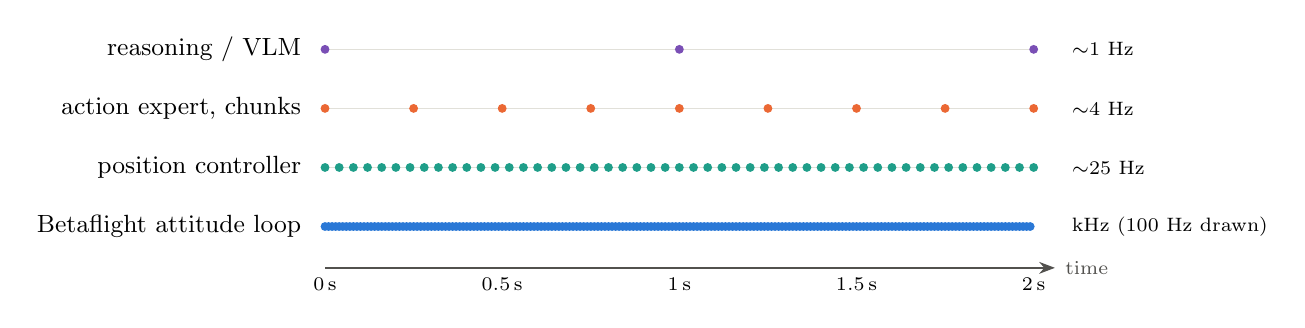
\begin{tikzpicture}[x=0.9cm,y=0.75cm,every node/.style={font=\scriptsize}]
\foreach \y/\n/\r/\c in {3/{reasoning / VLM}/5/cD, 2/{action expert, chunks}/1.25/cB, 1/{position controller}/0.2/cC, 0/{Betaflight attitude loop}/0.05/cA}{
  \node[anchor=east,font=\small] at (-0.2,\y) {\n};
  \draw[gridc] (0,\y)--(10,\y);
  \pgfmathsetmacro{\stp}{\r}
  \foreach \t in {0,\stp,...,10} \fill[\c] (\t,\y) circle (1.6pt);
}
\draw[arr] (0,-0.7)--(10.3,-0.7) node[right]{time};
\foreach \t in {0,2.5,5,7.5,10} \node[below] at (\t,-0.7) {\pgfmathparse{\t/5}\pgfmathprintnumber[fixed,precision=1]{\pgfmathresult}\,s};
\node[anchor=west] at (10.4,3) {$\sim$1~Hz};
\node[anchor=west] at (10.4,2) {$\sim$4~Hz};
\node[anchor=west] at (10.4,1) {$\sim$25~Hz};
\node[anchor=west] at (10.4,0) {kHz (100~Hz drawn)};
\end{tikzpicture}
\caption{Four control rates over two seconds of flight. A drone's attitude loop runs in the kilohertz range; a reasoning model runs about once per second. Each layer only needs to be as fast as the things it decides about.}
\label{fig:rates}
\end{figure}

\begin{bridgebox}
Your whoop already has this structure. Betaflight's attitude loop is System 1 at kilohertz rates; your Santana-style position controller sits above it. A VLA would add a slow layer on top. You do not replace control with learning; you put learning on top of control.
\end{bridgebox}

\subsection{What VLAs are good and bad at}
\textbf{Good at:} understanding open-ended instructions, recognising objects never seen in the robot data, coping with clutter, and producing smooth motions from demonstrations.

\textbf{Bad at:}
\begin{itemize}
\item \emph{Speed:} billions of parameters mean tens to hundreds of milliseconds per call.
\item \emph{Physics:} they map pictures to actions without an explicit model of what will happen, so they cannot check a plan before acting.
\item \emph{Long tasks:} errors accumulate (covariate shift again), and nothing tells the model that it has fallen off track.
\item \emph{Safety:} there is no guarantee; a confident wrong action looks the same as a correct one.
\item \emph{New robot bodies:} skills learned on arms transfer poorly to drones, because the dynamics are different. AirVLA (Section~\ref{sec:drones}) measured exactly this.
\end{itemize}
The next two chapters are answers to the long-task and physics problems: reasoning, and world models.

\begin{quizbox}
\begin{enumerate}[leftmargin=*]
\item How many network passes does a token-based VLA need for one 7-D action, and how many does a flow-matching VLA need for a 50-step chunk with 10 flow steps?
\item Why does the action expert in $\pi_0$ attend to the VLM rather than the other way round?
\item Name the layers of your whoop's control stack and their approximate rates.
\end{enumerate}
\emph{Answers: 1) seven (one per token), versus one VLM pass plus ten action-expert passes for 50 actions; 2) the VLM provides the understanding, and the actions must be conditioned on it, while the VLM does not need to know the noisy actions; 3) Betaflight attitude/rate loop (kHz), your position controller (tens of Hz), the ground-station planner (slower).}
\end{quizbox}

% --------------------------------------------------------------------
\section{Reasoning VLAs: thinking before acting}
\label{sec:rvla}

\subsection{Why make a robot think?}
A plain VLA maps ``what I see'' to ``what I do'' in one jump. That works for short tasks such as ``pick up the cube''. It struggles with ``tidy the table, but put the fragile things in the box first'', or with a scene it has never seen, because there is no step where the model works out \emph{what} to do before deciding \emph{how}. A reasoning VLA adds intermediate outputs between perception and action, just as chain-of-thought adds them between question and answer. Four flavours exist, depending on what the intermediate output looks like (Figure~\ref{fig:flavours}).

\begin{figure}[h]
\centering
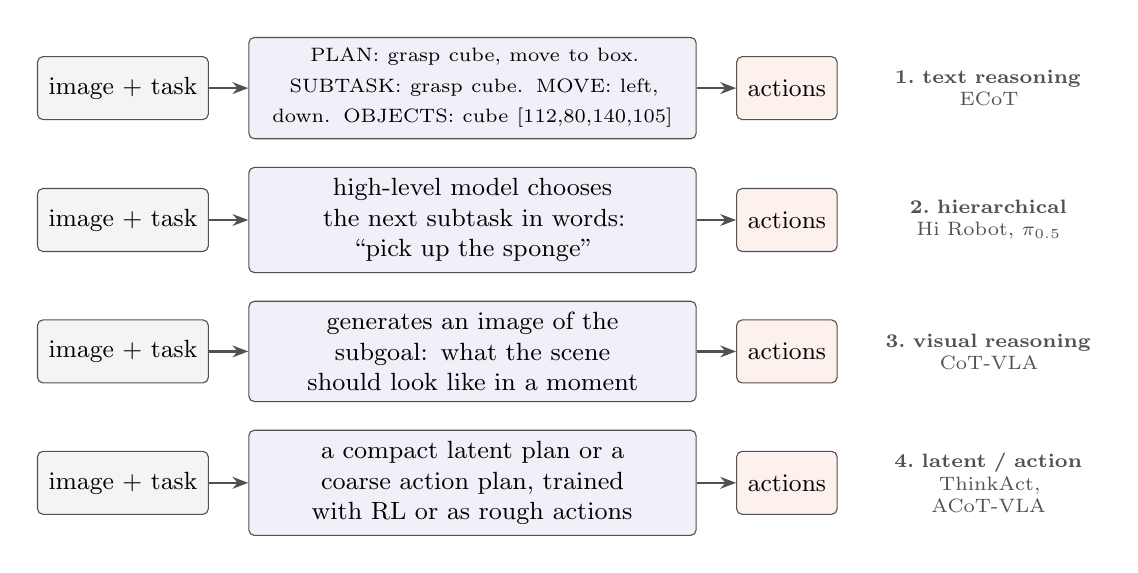
\begin{tikzpicture}[node distance=3mm, every node/.style={font=\small}]
\matrix[row sep=3.5mm, column sep=5mm] {
\node[bx=gray] (o1) {image + task}; & \node[bx=cD, text width=5.4cm] (r1) {\scriptsize PLAN: grasp cube, move to box. SUBTASK: grasp cube. MOVE: left, down. OBJECTS: cube [112,80,140,105]}; & \node[bx=cB] (a1) {actions}; & \node[lbl,text width=2.6cm,anchor=west] {\textbf{1.\ text reasoning}\\ECoT}; \\
\node[bx=gray] (o2) {image + task}; & \node[bx=cD, text width=5.4cm] (r2) {high-level model chooses the next subtask in words: ``pick up the sponge''}; & \node[bx=cB] (a2) {actions}; & \node[lbl,text width=2.6cm,anchor=west] {\textbf{2.\ hierarchical}\\Hi Robot, $\pi_{0.5}$}; \\
\node[bx=gray] (o3) {image + task}; & \node[bx=cD, text width=5.4cm] (r3) {generates an image of the subgoal: what the scene should look like in a moment}; & \node[bx=cB] (a3) {actions}; & \node[lbl,text width=2.6cm,anchor=west] {\textbf{3.\ visual reasoning}\\CoT-VLA}; \\
\node[bx=gray] (o4) {image + task}; & \node[bx=cD, text width=5.4cm] (r4) {a compact latent plan or a coarse action plan, trained with RL or as rough actions}; & \node[bx=cB] (a4) {actions}; & \node[lbl,text width=2.6cm,anchor=west] {\textbf{4.\ latent / action}\\ThinkAct, ACoT-VLA}; \\
};
\foreach \i in {1,2,3,4} {\draw[arr] (o\i)--(r\i); \draw[arr] (r\i)--(a\i);}
\end{tikzpicture}
\caption{Four flavours of reasoning VLAs, by what the model produces between seeing and acting.}
\label{fig:flavours}
\end{figure}

\subsection{Flavour 1: reasoning in text}
\begin{paperbox}{Zawalski et al.\ (2024), ``Robotic Control via Embodied Chain-of-Thought Reasoning'' (ECoT)}
Fine-tunes OpenVLA to write a structured reasoning trace before every action: the task, a high-level plan, the current subtask, a primitive movement in words (``move left''), the gripper's pixel position, and the objects in view with bounding boxes. The reasoning labels for the training data were generated automatically with pretrained detectors and a large language model, so no human wrote them. Result: about 28\% higher absolute success than OpenVLA on hard generalisation tasks, without extra robot data. Because the trace is in words, a human can read it and even correct the plan. Cost: hundreds of extra tokens per step make the policy much slower.
\end{paperbox}

Why does this help? The intermediate steps are \emph{grounded}: the bounding boxes and gripper positions force the model to locate things in the image before it moves. Each step is easier to learn than the whole jump, and steps learned on one task (``find the object'') are reused in others.

\begin{examplebox}
What an ECoT-style trace could look like for a drone (my illustration, not from a paper):\\[2pt]
\texttt{TASK: land on the red box.\ \ PLAN: rise above the table; find the red box; fly over it; descend.\ \ SUBTASK: find the red box.\ \ MOVE: rotate left.\ \ OBJECTS: red box [210,140,260,180], table [0,120,320,240].}\\[2pt]
The fast controller would only receive the last line of motion; the rest is the model's scratchpad.
\end{examplebox}

\subsection{Flavour 2: a planner that talks to a doer}
\begin{paperbox}{Shi et al.\ (2025), ``Hi Robot: Open-Ended Instruction Following with Hierarchical VLA Models''}
Splits the robot into a high-level VLM that reads complex instructions and live user feedback (``that's not trash'') and decides the next step in plain language, and a low-level VLA ($\pi_0$-style) that executes that step. Tested on single-arm, dual-arm and mobile robots for tasks such as clearing tables and making sandwiches. The interface between the two levels is a short sentence, which is easy to inspect.
\end{paperbox}
$\pi_{0.5}$ does the same inside a single model: it first predicts a subtask in text, then the actions for it.

\subsection{Flavour 3: reasoning in pictures}
\begin{paperbox}{Zhao et al.\ (CVPR 2025), ``CoT-VLA: Visual Chain-of-Thought Reasoning for VLA Models''}
A 7B model that can generate both images and actions. Before acting, it generates a \emph{subgoal image}: what the camera should see a few steps from now. It then generates a short action chunk to reach that image. The authors report 17\% better real-world success and 6\% better simulation results than the previous state of the art. The subgoal image is a small world-model prediction inside the policy, a first link between reasoning and world models.
\end{paperbox}

\subsection{Flavour 4: reasoning in latents or actions}
Words and pictures are not the only possible scratchpad. \textbf{ThinkAct} (2025) trains a multimodal LLM with reinforcement learning to produce reasoning plans that are rewarded when they lead to visually confirmed goal completion and consistent trajectories. The plan is then compressed into a latent vector that conditions a separate action model. \textbf{ACoT-VLA} (CVPR 2026) argues that robots should ``think'' directly in the action space: it first produces a coarse action plan and then refines it. Commercial systems also ``think'': Google DeepMind describes Gemini Robotics 1.5 as reasoning in natural language before producing motor commands.

\subsection{Problems that are still open}
\begin{watchbox}
\begin{itemize}[leftmargin=*]
\item \textbf{Latency.} A reasoning trace of a few hundred tokens takes a large fraction of a second. Hierarchical designs hide this by reasoning rarely and acting often.
\item \textbf{Faithfulness.} The written reasoning does not have to be the true cause of the action. A model can write a sensible plan and then do something else.
\item \textbf{No physics check.} A plan in words or pictures can be physically impossible (``fly through the gap'' when the gap is too narrow). Nothing in a reasoning VLA tests the plan against dynamics before it is executed.
\item \textbf{Labels.} Good reasoning labels for robot data are scarce. They are generated by other models (ECoT) or replaced by rewards (ThinkAct).
\end{itemize}
\end{watchbox}

The third point is where world models come in. A world model is a learned simulator: it can take a plan, imagine its outcome, and report back before the robot moves. That is the subject of Part IV.

\begin{quizbox}
\begin{enumerate}[leftmargin=*]
\item Name the four flavours of reasoning and one model for each.
\item Why do bounding boxes in ECoT's trace help the actions?
\item In what sense is CoT-VLA's subgoal image a world-model prediction?
\end{enumerate}
\emph{Answers: 1) text (ECoT), hierarchical (Hi Robot, $\pi_{0.5}$), visual (CoT-VLA), latent/action (ThinkAct, ACoT-VLA); 2) they force the model to locate the relevant objects before moving, which grounds the plan in the image; 3) it predicts the future observation that should result from acting, which is what a world model does.}
\end{quizbox}

\part{World models}
% ============================== PART IV ==============================
\section{What a world model is}
\label{sec:wm}

\subsection{Definition}
A world model is a learned predictor of the consequences of actions:
\begin{equation}
\hat p_\phi\big(s_{t+1}\mid s_t,a_t\big)\qquad\text{or, from pixels,}\qquad \hat p_\phi\big(o_{t+1:t+H}\mid o_{\le t},a_{t:t+H-1}\big).
\end{equation}
Given what the robot has seen and a sequence of actions it \emph{might} take, the model predicts what it would see and where it would be. It is the right-hand box of Figure~\ref{fig:loop}, learned from data, so the robot can query it without moving.

\begin{bridgebox}
You have already used a world model. The Santana-style controller on your whoop is built on a linear model of the hovering drone, $\ddot{\vect X}=f_1\vect U-f_2\dot{\vect X}$. That is a hand-derived world model with a few parameters that you identified from flight data. Fitting $\vect x_{t+1}=A\vect x_t+B\vect u_t$ by least squares is linear regression from the course book. Modern world models do the same thing with a neural network, in a learned latent space, from camera images.
\end{bridgebox}

\subsection{Four ways to use one}
\begin{figure}[h]
\centering
\begin{tikzpicture}[node distance=5mm and 7mm, every node/.style={font=\small}]
\node[bx=cD, minimum width=3.2cm, minimum height=1.2cm] (wm) {world model\\$\hat p(o',s'\mid s,a)$};
\node[bx=cA, above left=6mm and 4mm of wm, text width=3.6cm] (p) {\textbf{1.\ Plan:} try many action sequences in imagination, execute the best (MPC, \S\ref{sec:latentplan})};
\node[bx=cC, above right=6mm and 4mm of wm, text width=3.6cm] (t) {\textbf{2.\ Train a policy in imagination:} RL on dreamed rollouts (Dreamer, \S\ref{sec:dreamer})};
\node[bx=cB, below left=6mm and 4mm of wm, text width=3.6cm] (sim) {\textbf{3.\ Simulate:} generate training data or test scenes (Cosmos, Genie, \S\ref{sec:video})};
\node[bx=gray, below right=6mm and 4mm of wm, text width=3.6cm] (v) {\textbf{4.\ Verify:} check what another policy proposes before acting (\S\ref{sec:combine})};
\draw[arr] (wm)--(p); \draw[arr] (wm)--(t); \draw[arr] (wm)--(sim); \draw[arr] (wm)--(v);
\end{tikzpicture}
\caption{The same learned model can serve four purposes. Use 4 is the one that connects world models to reasoning VLAs.}
\label{fig:uses}
\end{figure}

\subsection{The central difficulty: compounding error}
\label{sec:compound}
A world model is applied to its own predictions: the predicted $\hat s_{t+1}$ is the input for predicting $\hat s_{t+2}$, and so on. Small one-step errors are fed back and grow. This is the same mechanism as covariate shift in behaviour cloning (Section~\ref{sec:il}): a model meets inputs it produced itself, which differ from its training data.

Figure~\ref{fig:compound} shows the effect on the simplest possible case. The true system rotates a 2-D state by $0.25$~rad per step. A linear model $\hat A$ is fitted by least squares from 25 noisy transitions. Its average one-step error is only \onestep, but after 10 imagined steps the average error is \errten\ and after 40 steps it is \errforty, more than ten times the one-step error.

\begin{figure}[h]
\centering
\begin{tikzpicture}
\begin{axis}[width=9.5cm,height=5cm, xmin=0, xmax=40, ymin=0, xlabel={imagined steps $h$}, ylabel={prediction error $\lVert \hat{\vect x}_h-\vect x_h\rVert$}, legend pos=north west]
\addplot[cD, very thick] table[x=h,y=mean]{figs/compound.dat}; \addlegendentry{mean over 200 starts}
\addplot[cD!50, thick, dashed] table[x=h,y=p90]{figs/compound.dat}; \addlegendentry{90th percentile}
\end{axis}
\end{tikzpicture}
\caption{Compounding error of a learned linear model rolled out on its own predictions. One-step accuracy says little about long-horizon accuracy.}
\label{fig:compound}
\end{figure}

\begin{probbox}{why the error grows: a derivation for linear models, and the $1/\sqrt N$ rule}
\textbf{Rollout error.} True system $\x_{h}=A^h\x_0$; model $\hat\x_h=\hat A^h\x_0$ with $\hat A=A+E$ and a small error $E$. Expanding the product and keeping terms with one $E$,
\[
\hat A^h=A^h+\sum_{j=0}^{h-1}A^{j}\,E\,A^{h-1-j}+(\text{terms with }E^2,E^3,\dots).
\]
For a rotation, $\lVert A\rVert=1$, so each of the $h$ terms has size at most $\lVert E\rVert$: the error is at most about $h\,\lVert E\rVert\,\lVert\x_0\rVert$, growing linearly with the horizon. In Figure~\ref{fig:compound} it grows more slowly than this bound because the rotated error terms partly cancel. For an unstable system ($\lVert A\rVert>1$) the same sum grows exponentially, which is why long imagined rollouts of fast, unstable dynamics such as a drone's are hard.

\textbf{Where $E$ comes from.} Least squares on $N$ noisy transitions estimates each entry of $A$ with a standard error proportional to $\sigma_{\text{noise}}/\sqrt N$, the same $1/\sqrt N$ law as for a sample mean ($\mathrm{Var}(\bar X)=\sigma^2/N$ by the variance rules in Part I). Four times the data halves the model error and so roughly halves the rollout error.
\end{probbox}

Three standard answers recur in the papers:
\begin{itemize}
\item \textbf{Plan over short horizons and replan often} (model predictive control, MPC): only the first action of each plan is executed, and fresh observations correct the model every step.
\item \textbf{Train on multi-step error}, not just one step, so the model learns to stay consistent with its own predictions.
\item \textbf{Predict in a latent space} that ignores irrelevant detail, so fewer things can go wrong.
\end{itemize}

\begin{quizbox}
\begin{enumerate}[leftmargin=*]
\item Which of the four uses in Figure~\ref{fig:uses} does your current whoop controller already make of its linear model?
\item Why does MPC tolerate an imperfect model better than executing one long plan open loop?
\end{enumerate}
\emph{Answers: 1) planning/control: the controller inverts the model to choose the command; 2) only the first action is used, and the next plan starts from the newly measured state, so errors cannot accumulate over the whole horizon.}
\end{quizbox}

% --------------------------------------------------------------------
\section{Learning latent dynamics: from ``World Models'' to Dreamer}
\label{sec:dreamer}

\subsection{The first deep world model}
\begin{paperbox}{Ha \& Schmidhuber (2018), ``World Models''}
Three parts: \textbf{V}, a VAE that compresses each frame into a small latent $\z$; \textbf{M}, a recurrent network that predicts the next $\z$ from the current one and the action; \textbf{C}, a tiny linear controller that acts from $\z$ and M's hidden state. The controller was trained entirely inside the ``dream'' produced by M and then transferred to the real game (a car-racing and a first-person shooting environment). It made the idea popular: learn a compact simulator from pixels, then learn to act inside it.
\end{paperbox}

\subsection{The recurrent state-space model (RSSM)}
PlaNet (Hafner et al., 2019) and its successors, the Dreamer family, use a model called the RSSM. Its state has two parts: a deterministic memory $\h_t$ (a GRU, a kind of RNN) that carries information over time, and a stochastic latent $\z_t$ that captures what is uncertain at this step.
\begin{align}
\text{memory:}\quad & \h_t=f_\phi(\h_{t-1},\z_{t-1},a_{t-1})\\
\text{prior (imagination):}\quad & \hat\z_t\sim p_\phi(\hat\z_t\mid\h_t)\\
\text{posterior (with the real image):}\quad & \z_t\sim q_\phi(\z_t\mid\h_t,o_t)\\
\text{decoders:}\quad & \hat o_t\sim p_\phi(o_t\mid\h_t,\z_t),\qquad \hat r_t\sim p_\phi(r_t\mid\h_t,\z_t)
\end{align}
The model is trained to reconstruct the images and rewards and to keep the prior close to the posterior:
\begin{equation}
\label{eq:rssmloss}\mathcal L=\sum_t\Big[-\log p(o_t\mid\h_t,\z_t)-\log p(r_t\mid\h_t,\z_t)+\beta\,\mathrm{KL}\big(q(\z_t\mid\h_t,o_t)\,\big\|\,p(\hat\z_t\mid\h_t)\big)\Big].
\end{equation}
The KL term is the key: it teaches the prior to predict, without seeing the image, what the posterior will find when it does see it. At planning time only the prior is used, so the model can roll forward without any images at all.

\begin{probbox}{Bayes' rule, prior and posterior, and the derivation of the ELBO}
\textbf{Bayes' rule.} From $p(z,o)=p(z)p(o\mid z)=p(o)p(z\mid o)$:
\[
p(z\mid o)=\frac{p(o\mid z)\,p(z)}{p(o)},\qquad p(o)=\int p(o\mid z)\,p(z)\,\mathrm dz .
\]
The \textbf{prior} $p(z)$ is the belief before seeing the image; the \textbf{posterior} $p(z\mid o)$ is the belief after. The integral for $p(o)$ runs over all possible latents, so the posterior cannot be computed exactly. A VAE or RSSM therefore learns an approximation $q(z\mid o)$, the encoder.

\textbf{Derivation of the ELBO} (evidence lower bound). Multiply and divide by $q$ inside the integral, then use Jensen ($\log\E\ge\E\log$, because $\log$ is concave):
\begin{align*}
\log p(o)&=\log\E_{z\sim q}\Big[\frac{p(o\mid z)\,p(z)}{q(z\mid o)}\Big]\ \ge\ \E_q\big[\log p(o\mid z)\big]+\E_q\Big[\log\frac{p(z)}{q(z\mid o)}\Big]\\
&=\underbrace{\E_q[\log p(o\mid z)]}_{\text{reconstruction}}-\underbrace{\mathrm{KL}\big(q(z\mid o)\,\|\,p(z)\big)}_{\text{stay close to the prior}} .
\end{align*}
Maximising this bound makes the data likely while keeping the encoder's guesses close to the prior. Its negative is the VAE loss, and the RSSM loss~\eqref{eq:rssmloss} is the same bound written for every time step, with the learned prior $p(\hat\z_t\mid\h_t)$ in place of a fixed $\mathcal N(0,1)$. One can show that the gap in the inequality is exactly $\mathrm{KL}\big(q(z\mid o)\,\|\,p(z\mid o)\big)$: the bound is tight when the encoder matches the true posterior.
\end{probbox}

\begin{figure}[h]
\centering
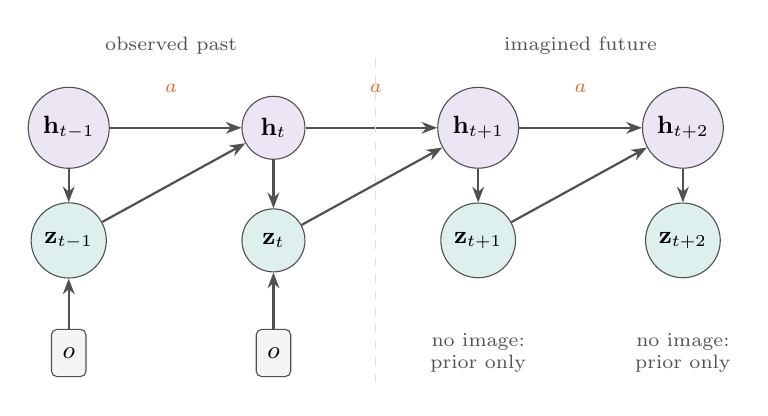
\begin{tikzpicture}[x=2.6cm,y=1.1cm,every node/.style={font=\small}]
\foreach \t/\lab in {0/{t-1},1/{t},2/{t+1},3/{t+2}} {
  \node[circle,draw=inkm,fill=cD!15,minimum size=8mm] (h\t) at (\t,0) {$\h_{\lab}$};
  \node[circle,draw=inkm,fill=cC!15,minimum size=8mm] (z\t) at (\t,-1.3) {$\z_{\lab}$};
  \draw[arr] (h\t)--(z\t);
}
\foreach \t in {0,1} {\node[bx=gray,minimum height=0.6cm] (o\t) at (\t,-2.6) {$o$}; \draw[arr] (o\t)--(z\t);}
\foreach \t in {2,3} {\node[lbl] at (\t,-2.6) {no image:\\prior only};}
\foreach \a/\b in {0/1,1/2,2/3} {\draw[arr] (h\a)--(h\b); \draw[arr] (z\a)--(h\b);
  \node[font=\scriptsize,color=cB] at (\a+0.5,0.45) {$a$};}
\draw[gridc, dashed] (1.5,0.8)--(1.5,-3);
\node[lbl] at (0.5,0.95) {observed past};
\node[lbl] at (2.5,0.95) {imagined future};
\end{tikzpicture}
\caption{The RSSM unrolled in time. In the past, each $\z$ is inferred from a real image. In the future, $\z$ comes from the prior alone, driven only by the chosen actions $a$.}
\label{fig:rssm}
\end{figure}

\subsection{Dreamer: learning to act inside the model}
Dreamer (Hafner et al., 2020) adds an actor--critic (Section~\ref{sec:rl}) that is trained \emph{only on imagined rollouts}: start from real latent states, imagine 15 or so steps with the prior and the actor's actions, predict the rewards, and train the critic and the actor on these dreams. Real interaction is used only to collect data and improve the model. \textbf{DreamerV3} (Hafner et al., 2023; published in Nature in 2025) made this robust across very different domains with a single set of hyperparameters, using tricks such as discrete latents (32 categorical variables with 32 classes each) and a ``symlog'' transform that tames very large and very small rewards. It was the first method to collect diamonds in Minecraft from scratch without human data.

\begin{paperbox}{Romero et al.\ (2025), ``Dream to Fly: Model-Based RL for Vision-Based Drone Flight'' (University of Zurich)}
Trains a quadrotor to fly through gates from raw camera pixels using DreamerV3, with the policy outputting collective thrust and body rates. The authors report that a model-free PPO baseline failed to learn from pixels in their setting, while the world-model approach succeeded, and that the policy transferred to a real quadrotor. The closest existing work to ``a world model for drone flight''. A 2026 follow-up from NTNU (Zanatta, Malczyk \& Alexis) studies how well such Dreamer world models generalise for depth-based quadrotor navigation, and finds that the latent size and training sequence length matter most.
\end{paperbox}

\subsection{Models without a decoder}
Reconstructing every pixel wastes capacity on textures that do not matter for control. \textbf{TD-MPC2} (Hansen et al., 2024) learns a latent model trained only to predict rewards, values and its own future latents, without a decoder, and plans with it (Section~\ref{sec:latentplan}). \textbf{MuZero} (Schrittwieser et al., 2020) did the same for board games and Atari. The cost: you can no longer look at what the model imagines, which matters if you want to \emph{explain} or \emph{verify} a plan.

\begin{quizbox}
\begin{enumerate}[leftmargin=*]
\item In the RSSM, which part carries memory over time and which part represents uncertainty?
\item What does the KL term teach the prior?
\item Why does Dreamer need far fewer real interactions than PPO?
\end{enumerate}
\emph{Answers: 1) $\h_t$ carries memory, $\z_t$ is stochastic; 2) to predict, without seeing the image, what the posterior will infer from it; 3) most of the policy's training happens on imagined rollouts, and real data is used only to improve the model.}
\end{quizbox}

% --------------------------------------------------------------------
\section{Planning with a learned model}
\label{sec:latentplan}

\subsection{Model predictive control with a world model}
The planning loop is the MPC you know from control engineering, with the learned model in place of the equations:
\begin{algbox}[MPC with a world model]
At every control step:
\begin{enumerate}[leftmargin=*]
\item Encode the current observation (and history) into a latent state.
\item Search for the action sequence $a_{t:t+H-1}$ whose imagined outcome has the lowest cost (or highest reward).
\item Execute only the first action (or the first few).
\item Observe again and repeat.
\end{enumerate}
\end{algbox}
The cost can be a learned reward, or, very commonly, the \textbf{distance between the predicted latent and the latent of a goal image}: ``make the future look like this picture''.

\subsection{The cross-entropy method (CEM)}
The search in step 2 is usually done by sampling, because the model is a neural network and gradients through long rollouts are unreliable. The \textbf{cross-entropy method} is the simplest and most used:
\begin{algbox}[Cross-entropy method]
Start with a Gaussian over action sequences, mean $\bm\mu$ and standard deviation $\bm\sigma$. Repeat a few times:
\begin{enumerate}[leftmargin=*]
\item Sample $N$ action sequences from $\mathcal N(\bm\mu,\bm\sigma^2)$.
\item Imagine each one with the world model and compute its cost.
\item Keep the $K$ best (the \emph{elites}).
\item Set $\bm\mu$ and $\bm\sigma$ to the mean and standard deviation of the elites.
\end{enumerate}
Return $\bm\mu$.
\end{algbox}

Figure~\ref{fig:cem} runs CEM on a toy: choose a 2-D waypoint that is close to the goal at $(1.6,1.2)$ and avoids a cost bump (an obstacle) at $(0.8,0.6)$. With $N=50$ samples and $K=8$ elites, the mean moves from the start $(0,0)$ to $(\cemmuxb,\cemmuyb)$ after two iterations and to $(\cemmuxc,\cemmuyc)$ after four: on the goal, with the spread shrinking around it. \textbf{MPPI} is a close relative that weights all samples by $e^{-\text{cost}/\lambda}$ instead of keeping a hard set of elites; TD-MPC2 uses it.

\begin{probbox}{CEM refits a Gaussian by maximum likelihood; MPPI is a softmax}
\textbf{Derivation.} Fit $\mathcal N(\mu,\sigma^2)$ to the $K$ elites $x_1,\dots,x_K$ by maximum likelihood (first box of Part I). The log-likelihood is
\[
\ell(\mu,\sigma^2)=-\frac K2\log(2\pi\sigma^2)-\sum_{i=1}^K\frac{(x_i-\mu)^2}{2\sigma^2}.
\]
Setting $\partial\ell/\partial\mu=\sum_i(x_i-\mu)/\sigma^2=0$ gives $\mu=\frac1K\sum_ix_i$, the sample mean. Setting $\partial\ell/\partial\sigma^2=-\frac{K}{2\sigma^2}+\frac{\sum_i(x_i-\mu)^2}{2\sigma^4}=0$ gives $\sigma^2=\frac1K\sum_i(x_i-\mu)^2$, the sample variance. So step 4 of CEM is maximum likelihood on the elites. The name: this is the same as minimising the cross-entropy between the elite distribution and the sampling distribution. (In the toy of Figure~\ref{fig:cem}, $0.02$ is added to $\sigma$ so that the search never collapses completely.)

\textbf{MPPI.} The weights $w_i=e^{-c_i/\lambda}/\sum_je^{-c_j/\lambda}$ are a softmax of the negative costs at temperature $\lambda$ (see the softmax box). As $\lambda\to0$ only the best sample counts; as $\lambda\to\infty$ all samples count equally. The new mean is $\sum_iw_ix_i$.
\end{probbox}

\begin{figure}[h]
\centering
\begin{tikzpicture}
\pgfplotsset{cemax/.style={width=5.4cm,height=5.4cm, xmin=-0.6, xmax=2.4, ymin=-0.6, ymax=2.4, axis equal image, grid=none, xtick={0,1,2}, ytick={0,1,2}}}
\begin{axis}[cemax, title={iteration 1}, ylabel={$a_2$}, xlabel={$a_1$}]
\addplot[cemcont] coordinates {(1.586,0.664) (1.556,0.673) (1.526,0.686) (1.495,0.706) (1.472,0.727) (1.450,0.749) (1.431,0.772) (1.408,0.802) (1.390,0.826) (1.375,0.848) (1.354,0.877) (1.333,0.908) (1.315,0.933) (1.299,0.953) (1.277,0.983) (1.254,1.013) (1.239,1.032) (1.218,1.058) (1.194,1.088) (1.179,1.108) (1.159,1.134) (1.137,1.164) (1.119,1.193) (1.104,1.222) (1.091,1.254) (1.084,1.284) (1.081,1.330) (1.088,1.375) (1.096,1.405) (1.108,1.435) (1.122,1.465) (1.140,1.495) (1.160,1.526) (1.179,1.550) (1.197,1.571) (1.224,1.598) (1.244,1.616) (1.269,1.637) (1.299,1.658) (1.330,1.676) (1.358,1.691) (1.390,1.706) (1.420,1.717) (1.450,1.727) (1.491,1.737) (1.526,1.743) (1.571,1.747) (1.616,1.747) (1.661,1.744) (1.707,1.737) (1.737,1.730) (1.767,1.722) (1.808,1.707) (1.842,1.691) (1.870,1.676) (1.895,1.661) (1.918,1.646) (1.948,1.623) (1.973,1.601) (1.993,1.581) (2.016,1.556) (2.038,1.529) (2.053,1.507) (2.070,1.480) (2.087,1.450) (2.102,1.420) (2.114,1.390) (2.128,1.345) (2.136,1.315) (2.143,1.269) (2.146,1.239) (2.148,1.194) (2.145,1.149) (2.142,1.119) (2.133,1.073) (2.125,1.043) (2.114,1.010) (2.098,0.973) (2.083,0.943) (2.068,0.916) (2.053,0.892) (2.031,0.862) (2.008,0.835) (1.992,0.817) (1.963,0.790) (1.942,0.772) (1.918,0.754) (1.887,0.734) (1.857,0.717) (1.827,0.702) (1.797,0.689) (1.767,0.679) (1.722,0.667) (1.691,0.662) (1.646,0.659) (1.601,0.662)};
\addplot[cemcont] coordinates {(2.400,0.800) (2.385,0.771) (2.368,0.742) (2.349,0.712) (2.329,0.681) (2.310,0.655) (2.294,0.636) (2.269,0.606) (2.249,0.585) (2.226,0.561) (2.204,0.540) (2.176,0.516) (2.157,0.501) (2.129,0.479) (2.098,0.457) (2.072,0.440) (2.047,0.425) (2.019,0.410) (1.990,0.395) (1.957,0.380) (1.920,0.365) (1.887,0.353) (1.857,0.343) (1.826,0.335) (1.782,0.324) (1.752,0.319) (1.707,0.312) (1.661,0.309) (1.616,0.308) (1.571,0.310) (1.526,0.317) (1.495,0.325) (1.465,0.338) (1.435,0.357) (1.412,0.380) (1.392,0.410) (1.378,0.440) (1.367,0.470) (1.358,0.501) (1.346,0.546) (1.338,0.576) (1.330,0.607) (1.317,0.651) (1.307,0.681) (1.296,0.712) (1.283,0.742) (1.269,0.772) (1.254,0.802) (1.237,0.832) (1.218,0.862) (1.197,0.892) (1.179,0.916) (1.161,0.938) (1.134,0.967) (1.118,0.983) (1.088,1.010) (1.067,1.028) (1.043,1.047) (1.013,1.069) (0.984,1.088) (0.960,1.104) (0.935,1.119) (0.908,1.135) (0.877,1.153) (0.847,1.172) (0.817,1.192) (0.796,1.209) (0.772,1.234) (0.757,1.254) (0.742,1.286) (0.732,1.330) (0.732,1.375) (0.737,1.420) (0.744,1.450) (0.757,1.495) (0.768,1.526) (0.780,1.556) (0.793,1.586) (0.808,1.616) (0.825,1.646) (0.843,1.676) (0.862,1.706) (0.877,1.727) (0.896,1.752) (0.921,1.782) (0.938,1.801) (0.962,1.827) (0.983,1.847) (1.010,1.872) (1.028,1.888) (1.058,1.912) (1.087,1.933) (1.109,1.948) (1.134,1.963) (1.164,1.981) (1.194,1.997) (1.224,2.012) (1.254,2.025) (1.288,2.038) (1.330,2.053) (1.360,2.062) (1.390,2.069) (1.435,2.079) (1.465,2.084) (1.511,2.090) (1.556,2.093) (1.601,2.094) (1.646,2.093) (1.691,2.090) (1.737,2.084) (1.767,2.079) (1.812,2.069) (1.842,2.061) (1.872,2.052) (1.912,2.038) (1.948,2.024) (1.978,2.011) (2.008,1.996) (2.038,1.980) (2.067,1.963) (2.091,1.948) (2.114,1.932) (2.144,1.910) (2.172,1.887) (2.190,1.872) (2.219,1.846) (2.238,1.827) (2.264,1.799) (2.279,1.782) (2.304,1.752) (2.325,1.724) (2.340,1.703) (2.357,1.676) (2.375,1.646) (2.392,1.616)};
\addplot[cemcont] coordinates {(2.400,0.273) (2.370,0.247) (2.347,0.229) (2.325,0.213) (2.294,0.191) (2.264,0.171) (2.237,0.154) (2.211,0.139) (2.184,0.124) (2.156,0.109) (2.125,0.093) (2.092,0.078) (2.056,0.063) (2.023,0.051) (1.993,0.040) (1.963,0.030) (1.921,0.018) (1.887,0.009) (1.857,0.003) (1.812,-0.006) (1.776,-0.012) (1.737,-0.017) (1.691,-0.021) (1.646,-0.024) (1.601,-0.025) (1.556,-0.024) (1.511,-0.021) (1.465,-0.017) (1.433,-0.012) (1.390,-0.004) (1.357,0.003) (1.315,0.015) (1.284,0.026) (1.254,0.040) (1.224,0.059) (1.202,0.078) (1.180,0.109) (1.171,0.139) (1.169,0.184) (1.177,0.229) (1.185,0.259) (1.194,0.294) (1.205,0.335) (1.212,0.365) (1.221,0.410) (1.225,0.440) (1.230,0.485) (1.231,0.531) (1.229,0.576) (1.224,0.612) (1.217,0.651) (1.209,0.681) (1.194,0.725) (1.180,0.757) (1.165,0.787) (1.149,0.814) (1.134,0.836) (1.114,0.862) (1.088,0.891) (1.072,0.908) (1.043,0.933) (1.018,0.953) (0.996,0.968) (0.968,0.985) (0.938,1.000) (0.908,1.014) (0.869,1.028) (0.832,1.039) (0.802,1.046) (0.757,1.054) (0.723,1.058) (0.681,1.062) (0.636,1.064) (0.591,1.065) (0.546,1.066) (0.501,1.072) (0.470,1.081) (0.440,1.098) (0.420,1.119) (0.403,1.149) (0.393,1.179) (0.385,1.224) (0.383,1.269) (0.384,1.315) (0.387,1.360) (0.393,1.405) (0.399,1.435) (0.408,1.480) (0.415,1.511) (0.425,1.546) (0.438,1.586) (0.448,1.616) (0.459,1.646) (0.472,1.676) (0.485,1.708) (0.501,1.740) (0.516,1.769) (0.531,1.797) (0.548,1.827) (0.567,1.857) (0.586,1.887) (0.606,1.916) (0.621,1.936) (0.642,1.963) (0.666,1.993) (0.681,2.010) (0.707,2.038) (0.727,2.059) (0.752,2.083) (0.772,2.102) (0.801,2.129) (0.819,2.144) (0.847,2.166) (0.877,2.189) (0.899,2.204) (0.923,2.220) (0.953,2.240) (0.983,2.258) (1.013,2.275) (1.043,2.291) (1.073,2.306) (1.104,2.320) (1.134,2.332) (1.164,2.344) (1.194,2.355) (1.237,2.370) (1.269,2.379) (1.299,2.387) (1.345,2.398)};
\addplot[cemcont] coordinates {(1.845,2.400) (1.887,2.391) (1.918,2.383) (1.963,2.370) (1.993,2.360) (2.023,2.349) (2.053,2.338) (2.085,2.325) (2.119,2.310) (2.150,2.294) (2.179,2.279) (2.206,2.264) (2.234,2.248) (2.264,2.229) (2.294,2.209) (2.322,2.189) (2.343,2.174) (2.370,2.153) (2.398,2.129)};
\addplot[cemcont] coordinates {(2.400,-0.164) (2.370,-0.181) (2.340,-0.197) (2.310,-0.213) (2.279,-0.228) (2.249,-0.242) (2.219,-0.255) (2.186,-0.268) (2.147,-0.283) (2.114,-0.295) (2.083,-0.305) (2.053,-0.315) (2.008,-0.328) (1.978,-0.335) (1.942,-0.344) (1.903,-0.352) (1.865,-0.359) (1.827,-0.365) (1.782,-0.371) (1.751,-0.374) (1.707,-0.378) (1.661,-0.380) (1.616,-0.381) (1.571,-0.381) (1.526,-0.379) (1.480,-0.377) (1.449,-0.374) (1.405,-0.369) (1.360,-0.363) (1.330,-0.358) (1.284,-0.349) (1.254,-0.343) (1.209,-0.332) (1.179,-0.324) (1.143,-0.314) (1.104,-0.301) (1.073,-0.290) (1.043,-0.279) (1.013,-0.267) (0.980,-0.253) (0.947,-0.238) (0.916,-0.223) (0.887,-0.208) (0.860,-0.193) (0.832,-0.177) (0.802,-0.157) (0.772,-0.136) (0.747,-0.118) (0.727,-0.101) (0.696,-0.074) (0.680,-0.057) (0.654,-0.027) (0.636,0.001) (0.623,0.033) (0.636,0.078) (0.660,0.093) (0.696,0.107) (0.727,0.115) (0.757,0.125) (0.800,0.139) (0.832,0.151) (0.862,0.164) (0.892,0.179) (0.923,0.196) (0.950,0.214) (0.970,0.229) (0.998,0.253) (1.020,0.274) (1.043,0.301) (1.058,0.320) (1.078,0.350) (1.095,0.380) (1.109,0.410) (1.120,0.440) (1.132,0.485) (1.137,0.516) (1.141,0.561) (1.139,0.606) (1.134,0.639) (1.123,0.681) (1.112,0.712) (1.099,0.742) (1.082,0.772) (1.061,0.802) (1.043,0.823) (1.019,0.847) (0.998,0.866) (0.968,0.888) (0.938,0.906) (0.908,0.920) (0.877,0.932) (0.847,0.941) (0.802,0.949) (0.757,0.952) (0.712,0.951) (0.666,0.944) (0.636,0.937) (0.594,0.923) (0.561,0.908) (0.531,0.892) (0.507,0.877) (0.485,0.862) (0.455,0.838) (0.432,0.817) (0.410,0.795) (0.390,0.772) (0.366,0.742) (0.350,0.719) (0.335,0.696) (0.315,0.666) (0.295,0.636) (0.274,0.607) (0.255,0.591) (0.214,0.586) (0.184,0.605) (0.169,0.621) (0.147,0.651) (0.128,0.681) (0.113,0.712) (0.100,0.742) (0.088,0.772) (0.077,0.802) (0.064,0.847) (0.056,0.877) (0.048,0.911) (0.040,0.953) (0.033,0.997) (0.029,1.028) (0.025,1.073) (0.021,1.119) (0.019,1.164) (0.019,1.209) (0.020,1.254) (0.022,1.299) (0.026,1.345) (0.030,1.390) (0.034,1.420) (0.041,1.465) (0.048,1.503) (0.056,1.541) (0.063,1.572) (0.075,1.616) (0.083,1.646) (0.093,1.680) (0.107,1.722) (0.118,1.752) (0.130,1.782) (0.142,1.812) (0.155,1.842) (0.169,1.872) (0.184,1.903) (0.199,1.933) (0.215,1.963) (0.232,1.993) (0.250,2.023) (0.269,2.053) (0.289,2.083) (0.305,2.106) (0.320,2.129) (0.343,2.159) (0.365,2.187) (0.380,2.206) (0.404,2.234) (0.425,2.258) (0.445,2.279) (0.470,2.306) (0.489,2.325) (0.516,2.351) (0.536,2.370) (0.561,2.392)};
\addplot[cemcont] coordinates {(0.728,-0.600) (0.698,-0.585) (0.669,-0.570) (0.640,-0.555) (0.613,-0.540) (0.587,-0.525) (0.561,-0.509) (0.531,-0.490) (0.501,-0.471) (0.470,-0.450) (0.447,-0.434) (0.425,-0.419) (0.395,-0.396) (0.366,-0.374) (0.347,-0.359) (0.320,-0.336) (0.293,-0.314) (0.274,-0.298) (0.244,-0.270) (0.226,-0.253) (0.199,-0.227) (0.180,-0.208) (0.154,-0.181) (0.136,-0.163) (0.109,-0.133) (0.093,-0.115) (0.070,-0.087) (0.048,-0.062) (0.033,-0.042) (0.009,-0.012) (-0.012,0.016) (-0.027,0.037) (-0.045,0.063) (-0.066,0.093) (-0.086,0.124) (-0.103,0.151) (-0.118,0.176) (-0.133,0.201) (-0.148,0.229) (-0.165,0.259) (-0.181,0.289) (-0.196,0.320) (-0.210,0.350) (-0.224,0.380) (-0.238,0.412) (-0.253,0.448) (-0.268,0.485) (-0.279,0.516) (-0.290,0.546) (-0.300,0.576) (-0.314,0.618) (-0.323,0.651) (-0.332,0.681) (-0.343,0.727) (-0.350,0.757) (-0.359,0.796) (-0.366,0.832) (-0.374,0.877) (-0.378,0.908) (-0.385,0.953) (-0.389,0.990) (-0.393,1.028) (-0.396,1.073) (-0.398,1.119) (-0.400,1.164) (-0.400,1.209) (-0.399,1.254) (-0.398,1.299) (-0.395,1.345) (-0.391,1.390) (-0.388,1.420) (-0.382,1.465) (-0.376,1.511) (-0.371,1.541) (-0.362,1.586) (-0.356,1.616) (-0.346,1.661) (-0.339,1.691) (-0.329,1.729) (-0.318,1.767) (-0.309,1.797) (-0.298,1.829) (-0.284,1.872) (-0.273,1.903) (-0.261,1.933) (-0.249,1.963) (-0.236,1.993) (-0.223,2.023) (-0.208,2.055) (-0.193,2.086) (-0.178,2.116) (-0.163,2.145) (-0.147,2.174) (-0.130,2.204) (-0.112,2.234) (-0.093,2.264) (-0.074,2.294) (-0.057,2.320) (-0.042,2.342) (-0.022,2.370) (0.000,2.400)};
\addplot[cemcont] coordinates {(0.772,0.304) (0.802,0.307) (0.847,0.316) (0.877,0.327) (0.908,0.343) (0.938,0.363) (0.957,0.380) (0.983,0.408) (0.998,0.428) (1.014,0.455) (1.028,0.487) (1.040,0.531) (1.044,0.561) (1.044,0.606) (1.039,0.636) (1.028,0.674) (1.013,0.708) (0.998,0.733) (0.980,0.757) (0.953,0.784) (0.930,0.802) (0.906,0.817) (0.874,0.832) (0.832,0.845) (0.802,0.850) (0.757,0.851) (0.727,0.847) (0.681,0.835) (0.651,0.823) (0.621,0.805) (0.597,0.787) (0.576,0.768) (0.553,0.742) (0.533,0.712) (0.518,0.681) (0.507,0.651) (0.500,0.621) (0.496,0.576) (0.499,0.531) (0.506,0.501) (0.516,0.470) (0.531,0.440) (0.551,0.410) (0.576,0.382) (0.595,0.365) (0.621,0.346) (0.651,0.330) (0.681,0.318) (0.727,0.307) (0.759,0.305)};
\addplot[cemcont] coordinates {(-0.061,-0.600) (-0.087,-0.576) (-0.109,-0.555) (-0.133,-0.531) (-0.154,-0.510) (-0.178,-0.485) (-0.197,-0.464) (-0.223,-0.436) (-0.238,-0.419) (-0.264,-0.389) (-0.283,-0.366) (-0.302,-0.344) (-0.326,-0.314) (-0.344,-0.291) (-0.361,-0.268) (-0.383,-0.238) (-0.404,-0.209) (-0.419,-0.187) (-0.435,-0.163) (-0.455,-0.133) (-0.474,-0.103) (-0.493,-0.072) (-0.510,-0.045) (-0.525,-0.019) (-0.540,0.008) (-0.555,0.035) (-0.570,0.063) (-0.585,0.093)};
\addplot[cemcont] coordinates {(-0.600,2.277) (-0.585,2.307) (-0.570,2.337) (-0.555,2.365) (-0.540,2.392)};
\addplot[cemcont] coordinates {(0.742,0.455) (0.787,0.449) (0.825,0.455) (0.858,0.470) (0.877,0.485) (0.902,0.516) (0.916,0.546) (0.922,0.591) (0.914,0.636) (0.898,0.666) (0.877,0.690) (0.847,0.711) (0.817,0.722) (0.772,0.726) (0.727,0.714) (0.697,0.696) (0.681,0.681) (0.660,0.651) (0.648,0.621) (0.645,0.576) (0.651,0.543) (0.666,0.512) (0.688,0.485) (0.712,0.468) (0.742,0.455)};

\addplot[only marks, mark=*, mark size=1.2pt, color=cA!60] table{figs/cem_all_a.dat};
\addplot[only marks, mark=*, mark size=1.8pt, color=cB] table{figs/cem_el_a.dat};
\addplot[only marks, mark=x, mark size=4pt, very thick, color=black] coordinates {(\cemmuxa,\cemmuya)};
\addplot[only marks, mark=star, mark size=4pt, color=cC, very thick] coordinates {(1.6,1.2)};
\end{axis}
\begin{axis}[cemax, xshift=5.2cm, title={iteration 3}, yticklabels={}, xlabel={$a_1$}]
\addplot[cemcont] coordinates {(1.586,0.664) (1.556,0.673) (1.526,0.686) (1.495,0.706) (1.472,0.727) (1.450,0.749) (1.431,0.772) (1.408,0.802) (1.390,0.826) (1.375,0.848) (1.354,0.877) (1.333,0.908) (1.315,0.933) (1.299,0.953) (1.277,0.983) (1.254,1.013) (1.239,1.032) (1.218,1.058) (1.194,1.088) (1.179,1.108) (1.159,1.134) (1.137,1.164) (1.119,1.193) (1.104,1.222) (1.091,1.254) (1.084,1.284) (1.081,1.330) (1.088,1.375) (1.096,1.405) (1.108,1.435) (1.122,1.465) (1.140,1.495) (1.160,1.526) (1.179,1.550) (1.197,1.571) (1.224,1.598) (1.244,1.616) (1.269,1.637) (1.299,1.658) (1.330,1.676) (1.358,1.691) (1.390,1.706) (1.420,1.717) (1.450,1.727) (1.491,1.737) (1.526,1.743) (1.571,1.747) (1.616,1.747) (1.661,1.744) (1.707,1.737) (1.737,1.730) (1.767,1.722) (1.808,1.707) (1.842,1.691) (1.870,1.676) (1.895,1.661) (1.918,1.646) (1.948,1.623) (1.973,1.601) (1.993,1.581) (2.016,1.556) (2.038,1.529) (2.053,1.507) (2.070,1.480) (2.087,1.450) (2.102,1.420) (2.114,1.390) (2.128,1.345) (2.136,1.315) (2.143,1.269) (2.146,1.239) (2.148,1.194) (2.145,1.149) (2.142,1.119) (2.133,1.073) (2.125,1.043) (2.114,1.010) (2.098,0.973) (2.083,0.943) (2.068,0.916) (2.053,0.892) (2.031,0.862) (2.008,0.835) (1.992,0.817) (1.963,0.790) (1.942,0.772) (1.918,0.754) (1.887,0.734) (1.857,0.717) (1.827,0.702) (1.797,0.689) (1.767,0.679) (1.722,0.667) (1.691,0.662) (1.646,0.659) (1.601,0.662)};
\addplot[cemcont] coordinates {(2.400,0.800) (2.385,0.771) (2.368,0.742) (2.349,0.712) (2.329,0.681) (2.310,0.655) (2.294,0.636) (2.269,0.606) (2.249,0.585) (2.226,0.561) (2.204,0.540) (2.176,0.516) (2.157,0.501) (2.129,0.479) (2.098,0.457) (2.072,0.440) (2.047,0.425) (2.019,0.410) (1.990,0.395) (1.957,0.380) (1.920,0.365) (1.887,0.353) (1.857,0.343) (1.826,0.335) (1.782,0.324) (1.752,0.319) (1.707,0.312) (1.661,0.309) (1.616,0.308) (1.571,0.310) (1.526,0.317) (1.495,0.325) (1.465,0.338) (1.435,0.357) (1.412,0.380) (1.392,0.410) (1.378,0.440) (1.367,0.470) (1.358,0.501) (1.346,0.546) (1.338,0.576) (1.330,0.607) (1.317,0.651) (1.307,0.681) (1.296,0.712) (1.283,0.742) (1.269,0.772) (1.254,0.802) (1.237,0.832) (1.218,0.862) (1.197,0.892) (1.179,0.916) (1.161,0.938) (1.134,0.967) (1.118,0.983) (1.088,1.010) (1.067,1.028) (1.043,1.047) (1.013,1.069) (0.984,1.088) (0.960,1.104) (0.935,1.119) (0.908,1.135) (0.877,1.153) (0.847,1.172) (0.817,1.192) (0.796,1.209) (0.772,1.234) (0.757,1.254) (0.742,1.286) (0.732,1.330) (0.732,1.375) (0.737,1.420) (0.744,1.450) (0.757,1.495) (0.768,1.526) (0.780,1.556) (0.793,1.586) (0.808,1.616) (0.825,1.646) (0.843,1.676) (0.862,1.706) (0.877,1.727) (0.896,1.752) (0.921,1.782) (0.938,1.801) (0.962,1.827) (0.983,1.847) (1.010,1.872) (1.028,1.888) (1.058,1.912) (1.087,1.933) (1.109,1.948) (1.134,1.963) (1.164,1.981) (1.194,1.997) (1.224,2.012) (1.254,2.025) (1.288,2.038) (1.330,2.053) (1.360,2.062) (1.390,2.069) (1.435,2.079) (1.465,2.084) (1.511,2.090) (1.556,2.093) (1.601,2.094) (1.646,2.093) (1.691,2.090) (1.737,2.084) (1.767,2.079) (1.812,2.069) (1.842,2.061) (1.872,2.052) (1.912,2.038) (1.948,2.024) (1.978,2.011) (2.008,1.996) (2.038,1.980) (2.067,1.963) (2.091,1.948) (2.114,1.932) (2.144,1.910) (2.172,1.887) (2.190,1.872) (2.219,1.846) (2.238,1.827) (2.264,1.799) (2.279,1.782) (2.304,1.752) (2.325,1.724) (2.340,1.703) (2.357,1.676) (2.375,1.646) (2.392,1.616)};
\addplot[cemcont] coordinates {(2.400,0.273) (2.370,0.247) (2.347,0.229) (2.325,0.213) (2.294,0.191) (2.264,0.171) (2.237,0.154) (2.211,0.139) (2.184,0.124) (2.156,0.109) (2.125,0.093) (2.092,0.078) (2.056,0.063) (2.023,0.051) (1.993,0.040) (1.963,0.030) (1.921,0.018) (1.887,0.009) (1.857,0.003) (1.812,-0.006) (1.776,-0.012) (1.737,-0.017) (1.691,-0.021) (1.646,-0.024) (1.601,-0.025) (1.556,-0.024) (1.511,-0.021) (1.465,-0.017) (1.433,-0.012) (1.390,-0.004) (1.357,0.003) (1.315,0.015) (1.284,0.026) (1.254,0.040) (1.224,0.059) (1.202,0.078) (1.180,0.109) (1.171,0.139) (1.169,0.184) (1.177,0.229) (1.185,0.259) (1.194,0.294) (1.205,0.335) (1.212,0.365) (1.221,0.410) (1.225,0.440) (1.230,0.485) (1.231,0.531) (1.229,0.576) (1.224,0.612) (1.217,0.651) (1.209,0.681) (1.194,0.725) (1.180,0.757) (1.165,0.787) (1.149,0.814) (1.134,0.836) (1.114,0.862) (1.088,0.891) (1.072,0.908) (1.043,0.933) (1.018,0.953) (0.996,0.968) (0.968,0.985) (0.938,1.000) (0.908,1.014) (0.869,1.028) (0.832,1.039) (0.802,1.046) (0.757,1.054) (0.723,1.058) (0.681,1.062) (0.636,1.064) (0.591,1.065) (0.546,1.066) (0.501,1.072) (0.470,1.081) (0.440,1.098) (0.420,1.119) (0.403,1.149) (0.393,1.179) (0.385,1.224) (0.383,1.269) (0.384,1.315) (0.387,1.360) (0.393,1.405) (0.399,1.435) (0.408,1.480) (0.415,1.511) (0.425,1.546) (0.438,1.586) (0.448,1.616) (0.459,1.646) (0.472,1.676) (0.485,1.708) (0.501,1.740) (0.516,1.769) (0.531,1.797) (0.548,1.827) (0.567,1.857) (0.586,1.887) (0.606,1.916) (0.621,1.936) (0.642,1.963) (0.666,1.993) (0.681,2.010) (0.707,2.038) (0.727,2.059) (0.752,2.083) (0.772,2.102) (0.801,2.129) (0.819,2.144) (0.847,2.166) (0.877,2.189) (0.899,2.204) (0.923,2.220) (0.953,2.240) (0.983,2.258) (1.013,2.275) (1.043,2.291) (1.073,2.306) (1.104,2.320) (1.134,2.332) (1.164,2.344) (1.194,2.355) (1.237,2.370) (1.269,2.379) (1.299,2.387) (1.345,2.398)};
\addplot[cemcont] coordinates {(1.845,2.400) (1.887,2.391) (1.918,2.383) (1.963,2.370) (1.993,2.360) (2.023,2.349) (2.053,2.338) (2.085,2.325) (2.119,2.310) (2.150,2.294) (2.179,2.279) (2.206,2.264) (2.234,2.248) (2.264,2.229) (2.294,2.209) (2.322,2.189) (2.343,2.174) (2.370,2.153) (2.398,2.129)};
\addplot[cemcont] coordinates {(2.400,-0.164) (2.370,-0.181) (2.340,-0.197) (2.310,-0.213) (2.279,-0.228) (2.249,-0.242) (2.219,-0.255) (2.186,-0.268) (2.147,-0.283) (2.114,-0.295) (2.083,-0.305) (2.053,-0.315) (2.008,-0.328) (1.978,-0.335) (1.942,-0.344) (1.903,-0.352) (1.865,-0.359) (1.827,-0.365) (1.782,-0.371) (1.751,-0.374) (1.707,-0.378) (1.661,-0.380) (1.616,-0.381) (1.571,-0.381) (1.526,-0.379) (1.480,-0.377) (1.449,-0.374) (1.405,-0.369) (1.360,-0.363) (1.330,-0.358) (1.284,-0.349) (1.254,-0.343) (1.209,-0.332) (1.179,-0.324) (1.143,-0.314) (1.104,-0.301) (1.073,-0.290) (1.043,-0.279) (1.013,-0.267) (0.980,-0.253) (0.947,-0.238) (0.916,-0.223) (0.887,-0.208) (0.860,-0.193) (0.832,-0.177) (0.802,-0.157) (0.772,-0.136) (0.747,-0.118) (0.727,-0.101) (0.696,-0.074) (0.680,-0.057) (0.654,-0.027) (0.636,0.001) (0.623,0.033) (0.636,0.078) (0.660,0.093) (0.696,0.107) (0.727,0.115) (0.757,0.125) (0.800,0.139) (0.832,0.151) (0.862,0.164) (0.892,0.179) (0.923,0.196) (0.950,0.214) (0.970,0.229) (0.998,0.253) (1.020,0.274) (1.043,0.301) (1.058,0.320) (1.078,0.350) (1.095,0.380) (1.109,0.410) (1.120,0.440) (1.132,0.485) (1.137,0.516) (1.141,0.561) (1.139,0.606) (1.134,0.639) (1.123,0.681) (1.112,0.712) (1.099,0.742) (1.082,0.772) (1.061,0.802) (1.043,0.823) (1.019,0.847) (0.998,0.866) (0.968,0.888) (0.938,0.906) (0.908,0.920) (0.877,0.932) (0.847,0.941) (0.802,0.949) (0.757,0.952) (0.712,0.951) (0.666,0.944) (0.636,0.937) (0.594,0.923) (0.561,0.908) (0.531,0.892) (0.507,0.877) (0.485,0.862) (0.455,0.838) (0.432,0.817) (0.410,0.795) (0.390,0.772) (0.366,0.742) (0.350,0.719) (0.335,0.696) (0.315,0.666) (0.295,0.636) (0.274,0.607) (0.255,0.591) (0.214,0.586) (0.184,0.605) (0.169,0.621) (0.147,0.651) (0.128,0.681) (0.113,0.712) (0.100,0.742) (0.088,0.772) (0.077,0.802) (0.064,0.847) (0.056,0.877) (0.048,0.911) (0.040,0.953) (0.033,0.997) (0.029,1.028) (0.025,1.073) (0.021,1.119) (0.019,1.164) (0.019,1.209) (0.020,1.254) (0.022,1.299) (0.026,1.345) (0.030,1.390) (0.034,1.420) (0.041,1.465) (0.048,1.503) (0.056,1.541) (0.063,1.572) (0.075,1.616) (0.083,1.646) (0.093,1.680) (0.107,1.722) (0.118,1.752) (0.130,1.782) (0.142,1.812) (0.155,1.842) (0.169,1.872) (0.184,1.903) (0.199,1.933) (0.215,1.963) (0.232,1.993) (0.250,2.023) (0.269,2.053) (0.289,2.083) (0.305,2.106) (0.320,2.129) (0.343,2.159) (0.365,2.187) (0.380,2.206) (0.404,2.234) (0.425,2.258) (0.445,2.279) (0.470,2.306) (0.489,2.325) (0.516,2.351) (0.536,2.370) (0.561,2.392)};
\addplot[cemcont] coordinates {(0.728,-0.600) (0.698,-0.585) (0.669,-0.570) (0.640,-0.555) (0.613,-0.540) (0.587,-0.525) (0.561,-0.509) (0.531,-0.490) (0.501,-0.471) (0.470,-0.450) (0.447,-0.434) (0.425,-0.419) (0.395,-0.396) (0.366,-0.374) (0.347,-0.359) (0.320,-0.336) (0.293,-0.314) (0.274,-0.298) (0.244,-0.270) (0.226,-0.253) (0.199,-0.227) (0.180,-0.208) (0.154,-0.181) (0.136,-0.163) (0.109,-0.133) (0.093,-0.115) (0.070,-0.087) (0.048,-0.062) (0.033,-0.042) (0.009,-0.012) (-0.012,0.016) (-0.027,0.037) (-0.045,0.063) (-0.066,0.093) (-0.086,0.124) (-0.103,0.151) (-0.118,0.176) (-0.133,0.201) (-0.148,0.229) (-0.165,0.259) (-0.181,0.289) (-0.196,0.320) (-0.210,0.350) (-0.224,0.380) (-0.238,0.412) (-0.253,0.448) (-0.268,0.485) (-0.279,0.516) (-0.290,0.546) (-0.300,0.576) (-0.314,0.618) (-0.323,0.651) (-0.332,0.681) (-0.343,0.727) (-0.350,0.757) (-0.359,0.796) (-0.366,0.832) (-0.374,0.877) (-0.378,0.908) (-0.385,0.953) (-0.389,0.990) (-0.393,1.028) (-0.396,1.073) (-0.398,1.119) (-0.400,1.164) (-0.400,1.209) (-0.399,1.254) (-0.398,1.299) (-0.395,1.345) (-0.391,1.390) (-0.388,1.420) (-0.382,1.465) (-0.376,1.511) (-0.371,1.541) (-0.362,1.586) (-0.356,1.616) (-0.346,1.661) (-0.339,1.691) (-0.329,1.729) (-0.318,1.767) (-0.309,1.797) (-0.298,1.829) (-0.284,1.872) (-0.273,1.903) (-0.261,1.933) (-0.249,1.963) (-0.236,1.993) (-0.223,2.023) (-0.208,2.055) (-0.193,2.086) (-0.178,2.116) (-0.163,2.145) (-0.147,2.174) (-0.130,2.204) (-0.112,2.234) (-0.093,2.264) (-0.074,2.294) (-0.057,2.320) (-0.042,2.342) (-0.022,2.370) (0.000,2.400)};
\addplot[cemcont] coordinates {(0.772,0.304) (0.802,0.307) (0.847,0.316) (0.877,0.327) (0.908,0.343) (0.938,0.363) (0.957,0.380) (0.983,0.408) (0.998,0.428) (1.014,0.455) (1.028,0.487) (1.040,0.531) (1.044,0.561) (1.044,0.606) (1.039,0.636) (1.028,0.674) (1.013,0.708) (0.998,0.733) (0.980,0.757) (0.953,0.784) (0.930,0.802) (0.906,0.817) (0.874,0.832) (0.832,0.845) (0.802,0.850) (0.757,0.851) (0.727,0.847) (0.681,0.835) (0.651,0.823) (0.621,0.805) (0.597,0.787) (0.576,0.768) (0.553,0.742) (0.533,0.712) (0.518,0.681) (0.507,0.651) (0.500,0.621) (0.496,0.576) (0.499,0.531) (0.506,0.501) (0.516,0.470) (0.531,0.440) (0.551,0.410) (0.576,0.382) (0.595,0.365) (0.621,0.346) (0.651,0.330) (0.681,0.318) (0.727,0.307) (0.759,0.305)};
\addplot[cemcont] coordinates {(-0.061,-0.600) (-0.087,-0.576) (-0.109,-0.555) (-0.133,-0.531) (-0.154,-0.510) (-0.178,-0.485) (-0.197,-0.464) (-0.223,-0.436) (-0.238,-0.419) (-0.264,-0.389) (-0.283,-0.366) (-0.302,-0.344) (-0.326,-0.314) (-0.344,-0.291) (-0.361,-0.268) (-0.383,-0.238) (-0.404,-0.209) (-0.419,-0.187) (-0.435,-0.163) (-0.455,-0.133) (-0.474,-0.103) (-0.493,-0.072) (-0.510,-0.045) (-0.525,-0.019) (-0.540,0.008) (-0.555,0.035) (-0.570,0.063) (-0.585,0.093)};
\addplot[cemcont] coordinates {(-0.600,2.277) (-0.585,2.307) (-0.570,2.337) (-0.555,2.365) (-0.540,2.392)};
\addplot[cemcont] coordinates {(0.742,0.455) (0.787,0.449) (0.825,0.455) (0.858,0.470) (0.877,0.485) (0.902,0.516) (0.916,0.546) (0.922,0.591) (0.914,0.636) (0.898,0.666) (0.877,0.690) (0.847,0.711) (0.817,0.722) (0.772,0.726) (0.727,0.714) (0.697,0.696) (0.681,0.681) (0.660,0.651) (0.648,0.621) (0.645,0.576) (0.651,0.543) (0.666,0.512) (0.688,0.485) (0.712,0.468) (0.742,0.455)};

\addplot[only marks, mark=*, mark size=1.2pt, color=cA!60] table{figs/cem_all_b.dat};
\addplot[only marks, mark=*, mark size=1.8pt, color=cB] table{figs/cem_el_b.dat};
\addplot[only marks, mark=x, mark size=4pt, very thick, color=black] coordinates {(\cemmuxb,\cemmuyb)};
\addplot[only marks, mark=star, mark size=4pt, color=cC, very thick] coordinates {(1.6,1.2)};
\end{axis}
\begin{axis}[cemax, xshift=10.4cm, title={iteration 5}, yticklabels={}, xlabel={$a_1$}]
\addplot[cemcont] coordinates {(1.586,0.664) (1.556,0.673) (1.526,0.686) (1.495,0.706) (1.472,0.727) (1.450,0.749) (1.431,0.772) (1.408,0.802) (1.390,0.826) (1.375,0.848) (1.354,0.877) (1.333,0.908) (1.315,0.933) (1.299,0.953) (1.277,0.983) (1.254,1.013) (1.239,1.032) (1.218,1.058) (1.194,1.088) (1.179,1.108) (1.159,1.134) (1.137,1.164) (1.119,1.193) (1.104,1.222) (1.091,1.254) (1.084,1.284) (1.081,1.330) (1.088,1.375) (1.096,1.405) (1.108,1.435) (1.122,1.465) (1.140,1.495) (1.160,1.526) (1.179,1.550) (1.197,1.571) (1.224,1.598) (1.244,1.616) (1.269,1.637) (1.299,1.658) (1.330,1.676) (1.358,1.691) (1.390,1.706) (1.420,1.717) (1.450,1.727) (1.491,1.737) (1.526,1.743) (1.571,1.747) (1.616,1.747) (1.661,1.744) (1.707,1.737) (1.737,1.730) (1.767,1.722) (1.808,1.707) (1.842,1.691) (1.870,1.676) (1.895,1.661) (1.918,1.646) (1.948,1.623) (1.973,1.601) (1.993,1.581) (2.016,1.556) (2.038,1.529) (2.053,1.507) (2.070,1.480) (2.087,1.450) (2.102,1.420) (2.114,1.390) (2.128,1.345) (2.136,1.315) (2.143,1.269) (2.146,1.239) (2.148,1.194) (2.145,1.149) (2.142,1.119) (2.133,1.073) (2.125,1.043) (2.114,1.010) (2.098,0.973) (2.083,0.943) (2.068,0.916) (2.053,0.892) (2.031,0.862) (2.008,0.835) (1.992,0.817) (1.963,0.790) (1.942,0.772) (1.918,0.754) (1.887,0.734) (1.857,0.717) (1.827,0.702) (1.797,0.689) (1.767,0.679) (1.722,0.667) (1.691,0.662) (1.646,0.659) (1.601,0.662)};
\addplot[cemcont] coordinates {(2.400,0.800) (2.385,0.771) (2.368,0.742) (2.349,0.712) (2.329,0.681) (2.310,0.655) (2.294,0.636) (2.269,0.606) (2.249,0.585) (2.226,0.561) (2.204,0.540) (2.176,0.516) (2.157,0.501) (2.129,0.479) (2.098,0.457) (2.072,0.440) (2.047,0.425) (2.019,0.410) (1.990,0.395) (1.957,0.380) (1.920,0.365) (1.887,0.353) (1.857,0.343) (1.826,0.335) (1.782,0.324) (1.752,0.319) (1.707,0.312) (1.661,0.309) (1.616,0.308) (1.571,0.310) (1.526,0.317) (1.495,0.325) (1.465,0.338) (1.435,0.357) (1.412,0.380) (1.392,0.410) (1.378,0.440) (1.367,0.470) (1.358,0.501) (1.346,0.546) (1.338,0.576) (1.330,0.607) (1.317,0.651) (1.307,0.681) (1.296,0.712) (1.283,0.742) (1.269,0.772) (1.254,0.802) (1.237,0.832) (1.218,0.862) (1.197,0.892) (1.179,0.916) (1.161,0.938) (1.134,0.967) (1.118,0.983) (1.088,1.010) (1.067,1.028) (1.043,1.047) (1.013,1.069) (0.984,1.088) (0.960,1.104) (0.935,1.119) (0.908,1.135) (0.877,1.153) (0.847,1.172) (0.817,1.192) (0.796,1.209) (0.772,1.234) (0.757,1.254) (0.742,1.286) (0.732,1.330) (0.732,1.375) (0.737,1.420) (0.744,1.450) (0.757,1.495) (0.768,1.526) (0.780,1.556) (0.793,1.586) (0.808,1.616) (0.825,1.646) (0.843,1.676) (0.862,1.706) (0.877,1.727) (0.896,1.752) (0.921,1.782) (0.938,1.801) (0.962,1.827) (0.983,1.847) (1.010,1.872) (1.028,1.888) (1.058,1.912) (1.087,1.933) (1.109,1.948) (1.134,1.963) (1.164,1.981) (1.194,1.997) (1.224,2.012) (1.254,2.025) (1.288,2.038) (1.330,2.053) (1.360,2.062) (1.390,2.069) (1.435,2.079) (1.465,2.084) (1.511,2.090) (1.556,2.093) (1.601,2.094) (1.646,2.093) (1.691,2.090) (1.737,2.084) (1.767,2.079) (1.812,2.069) (1.842,2.061) (1.872,2.052) (1.912,2.038) (1.948,2.024) (1.978,2.011) (2.008,1.996) (2.038,1.980) (2.067,1.963) (2.091,1.948) (2.114,1.932) (2.144,1.910) (2.172,1.887) (2.190,1.872) (2.219,1.846) (2.238,1.827) (2.264,1.799) (2.279,1.782) (2.304,1.752) (2.325,1.724) (2.340,1.703) (2.357,1.676) (2.375,1.646) (2.392,1.616)};
\addplot[cemcont] coordinates {(2.400,0.273) (2.370,0.247) (2.347,0.229) (2.325,0.213) (2.294,0.191) (2.264,0.171) (2.237,0.154) (2.211,0.139) (2.184,0.124) (2.156,0.109) (2.125,0.093) (2.092,0.078) (2.056,0.063) (2.023,0.051) (1.993,0.040) (1.963,0.030) (1.921,0.018) (1.887,0.009) (1.857,0.003) (1.812,-0.006) (1.776,-0.012) (1.737,-0.017) (1.691,-0.021) (1.646,-0.024) (1.601,-0.025) (1.556,-0.024) (1.511,-0.021) (1.465,-0.017) (1.433,-0.012) (1.390,-0.004) (1.357,0.003) (1.315,0.015) (1.284,0.026) (1.254,0.040) (1.224,0.059) (1.202,0.078) (1.180,0.109) (1.171,0.139) (1.169,0.184) (1.177,0.229) (1.185,0.259) (1.194,0.294) (1.205,0.335) (1.212,0.365) (1.221,0.410) (1.225,0.440) (1.230,0.485) (1.231,0.531) (1.229,0.576) (1.224,0.612) (1.217,0.651) (1.209,0.681) (1.194,0.725) (1.180,0.757) (1.165,0.787) (1.149,0.814) (1.134,0.836) (1.114,0.862) (1.088,0.891) (1.072,0.908) (1.043,0.933) (1.018,0.953) (0.996,0.968) (0.968,0.985) (0.938,1.000) (0.908,1.014) (0.869,1.028) (0.832,1.039) (0.802,1.046) (0.757,1.054) (0.723,1.058) (0.681,1.062) (0.636,1.064) (0.591,1.065) (0.546,1.066) (0.501,1.072) (0.470,1.081) (0.440,1.098) (0.420,1.119) (0.403,1.149) (0.393,1.179) (0.385,1.224) (0.383,1.269) (0.384,1.315) (0.387,1.360) (0.393,1.405) (0.399,1.435) (0.408,1.480) (0.415,1.511) (0.425,1.546) (0.438,1.586) (0.448,1.616) (0.459,1.646) (0.472,1.676) (0.485,1.708) (0.501,1.740) (0.516,1.769) (0.531,1.797) (0.548,1.827) (0.567,1.857) (0.586,1.887) (0.606,1.916) (0.621,1.936) (0.642,1.963) (0.666,1.993) (0.681,2.010) (0.707,2.038) (0.727,2.059) (0.752,2.083) (0.772,2.102) (0.801,2.129) (0.819,2.144) (0.847,2.166) (0.877,2.189) (0.899,2.204) (0.923,2.220) (0.953,2.240) (0.983,2.258) (1.013,2.275) (1.043,2.291) (1.073,2.306) (1.104,2.320) (1.134,2.332) (1.164,2.344) (1.194,2.355) (1.237,2.370) (1.269,2.379) (1.299,2.387) (1.345,2.398)};
\addplot[cemcont] coordinates {(1.845,2.400) (1.887,2.391) (1.918,2.383) (1.963,2.370) (1.993,2.360) (2.023,2.349) (2.053,2.338) (2.085,2.325) (2.119,2.310) (2.150,2.294) (2.179,2.279) (2.206,2.264) (2.234,2.248) (2.264,2.229) (2.294,2.209) (2.322,2.189) (2.343,2.174) (2.370,2.153) (2.398,2.129)};
\addplot[cemcont] coordinates {(2.400,-0.164) (2.370,-0.181) (2.340,-0.197) (2.310,-0.213) (2.279,-0.228) (2.249,-0.242) (2.219,-0.255) (2.186,-0.268) (2.147,-0.283) (2.114,-0.295) (2.083,-0.305) (2.053,-0.315) (2.008,-0.328) (1.978,-0.335) (1.942,-0.344) (1.903,-0.352) (1.865,-0.359) (1.827,-0.365) (1.782,-0.371) (1.751,-0.374) (1.707,-0.378) (1.661,-0.380) (1.616,-0.381) (1.571,-0.381) (1.526,-0.379) (1.480,-0.377) (1.449,-0.374) (1.405,-0.369) (1.360,-0.363) (1.330,-0.358) (1.284,-0.349) (1.254,-0.343) (1.209,-0.332) (1.179,-0.324) (1.143,-0.314) (1.104,-0.301) (1.073,-0.290) (1.043,-0.279) (1.013,-0.267) (0.980,-0.253) (0.947,-0.238) (0.916,-0.223) (0.887,-0.208) (0.860,-0.193) (0.832,-0.177) (0.802,-0.157) (0.772,-0.136) (0.747,-0.118) (0.727,-0.101) (0.696,-0.074) (0.680,-0.057) (0.654,-0.027) (0.636,0.001) (0.623,0.033) (0.636,0.078) (0.660,0.093) (0.696,0.107) (0.727,0.115) (0.757,0.125) (0.800,0.139) (0.832,0.151) (0.862,0.164) (0.892,0.179) (0.923,0.196) (0.950,0.214) (0.970,0.229) (0.998,0.253) (1.020,0.274) (1.043,0.301) (1.058,0.320) (1.078,0.350) (1.095,0.380) (1.109,0.410) (1.120,0.440) (1.132,0.485) (1.137,0.516) (1.141,0.561) (1.139,0.606) (1.134,0.639) (1.123,0.681) (1.112,0.712) (1.099,0.742) (1.082,0.772) (1.061,0.802) (1.043,0.823) (1.019,0.847) (0.998,0.866) (0.968,0.888) (0.938,0.906) (0.908,0.920) (0.877,0.932) (0.847,0.941) (0.802,0.949) (0.757,0.952) (0.712,0.951) (0.666,0.944) (0.636,0.937) (0.594,0.923) (0.561,0.908) (0.531,0.892) (0.507,0.877) (0.485,0.862) (0.455,0.838) (0.432,0.817) (0.410,0.795) (0.390,0.772) (0.366,0.742) (0.350,0.719) (0.335,0.696) (0.315,0.666) (0.295,0.636) (0.274,0.607) (0.255,0.591) (0.214,0.586) (0.184,0.605) (0.169,0.621) (0.147,0.651) (0.128,0.681) (0.113,0.712) (0.100,0.742) (0.088,0.772) (0.077,0.802) (0.064,0.847) (0.056,0.877) (0.048,0.911) (0.040,0.953) (0.033,0.997) (0.029,1.028) (0.025,1.073) (0.021,1.119) (0.019,1.164) (0.019,1.209) (0.020,1.254) (0.022,1.299) (0.026,1.345) (0.030,1.390) (0.034,1.420) (0.041,1.465) (0.048,1.503) (0.056,1.541) (0.063,1.572) (0.075,1.616) (0.083,1.646) (0.093,1.680) (0.107,1.722) (0.118,1.752) (0.130,1.782) (0.142,1.812) (0.155,1.842) (0.169,1.872) (0.184,1.903) (0.199,1.933) (0.215,1.963) (0.232,1.993) (0.250,2.023) (0.269,2.053) (0.289,2.083) (0.305,2.106) (0.320,2.129) (0.343,2.159) (0.365,2.187) (0.380,2.206) (0.404,2.234) (0.425,2.258) (0.445,2.279) (0.470,2.306) (0.489,2.325) (0.516,2.351) (0.536,2.370) (0.561,2.392)};
\addplot[cemcont] coordinates {(0.728,-0.600) (0.698,-0.585) (0.669,-0.570) (0.640,-0.555) (0.613,-0.540) (0.587,-0.525) (0.561,-0.509) (0.531,-0.490) (0.501,-0.471) (0.470,-0.450) (0.447,-0.434) (0.425,-0.419) (0.395,-0.396) (0.366,-0.374) (0.347,-0.359) (0.320,-0.336) (0.293,-0.314) (0.274,-0.298) (0.244,-0.270) (0.226,-0.253) (0.199,-0.227) (0.180,-0.208) (0.154,-0.181) (0.136,-0.163) (0.109,-0.133) (0.093,-0.115) (0.070,-0.087) (0.048,-0.062) (0.033,-0.042) (0.009,-0.012) (-0.012,0.016) (-0.027,0.037) (-0.045,0.063) (-0.066,0.093) (-0.086,0.124) (-0.103,0.151) (-0.118,0.176) (-0.133,0.201) (-0.148,0.229) (-0.165,0.259) (-0.181,0.289) (-0.196,0.320) (-0.210,0.350) (-0.224,0.380) (-0.238,0.412) (-0.253,0.448) (-0.268,0.485) (-0.279,0.516) (-0.290,0.546) (-0.300,0.576) (-0.314,0.618) (-0.323,0.651) (-0.332,0.681) (-0.343,0.727) (-0.350,0.757) (-0.359,0.796) (-0.366,0.832) (-0.374,0.877) (-0.378,0.908) (-0.385,0.953) (-0.389,0.990) (-0.393,1.028) (-0.396,1.073) (-0.398,1.119) (-0.400,1.164) (-0.400,1.209) (-0.399,1.254) (-0.398,1.299) (-0.395,1.345) (-0.391,1.390) (-0.388,1.420) (-0.382,1.465) (-0.376,1.511) (-0.371,1.541) (-0.362,1.586) (-0.356,1.616) (-0.346,1.661) (-0.339,1.691) (-0.329,1.729) (-0.318,1.767) (-0.309,1.797) (-0.298,1.829) (-0.284,1.872) (-0.273,1.903) (-0.261,1.933) (-0.249,1.963) (-0.236,1.993) (-0.223,2.023) (-0.208,2.055) (-0.193,2.086) (-0.178,2.116) (-0.163,2.145) (-0.147,2.174) (-0.130,2.204) (-0.112,2.234) (-0.093,2.264) (-0.074,2.294) (-0.057,2.320) (-0.042,2.342) (-0.022,2.370) (0.000,2.400)};
\addplot[cemcont] coordinates {(0.772,0.304) (0.802,0.307) (0.847,0.316) (0.877,0.327) (0.908,0.343) (0.938,0.363) (0.957,0.380) (0.983,0.408) (0.998,0.428) (1.014,0.455) (1.028,0.487) (1.040,0.531) (1.044,0.561) (1.044,0.606) (1.039,0.636) (1.028,0.674) (1.013,0.708) (0.998,0.733) (0.980,0.757) (0.953,0.784) (0.930,0.802) (0.906,0.817) (0.874,0.832) (0.832,0.845) (0.802,0.850) (0.757,0.851) (0.727,0.847) (0.681,0.835) (0.651,0.823) (0.621,0.805) (0.597,0.787) (0.576,0.768) (0.553,0.742) (0.533,0.712) (0.518,0.681) (0.507,0.651) (0.500,0.621) (0.496,0.576) (0.499,0.531) (0.506,0.501) (0.516,0.470) (0.531,0.440) (0.551,0.410) (0.576,0.382) (0.595,0.365) (0.621,0.346) (0.651,0.330) (0.681,0.318) (0.727,0.307) (0.759,0.305)};
\addplot[cemcont] coordinates {(-0.061,-0.600) (-0.087,-0.576) (-0.109,-0.555) (-0.133,-0.531) (-0.154,-0.510) (-0.178,-0.485) (-0.197,-0.464) (-0.223,-0.436) (-0.238,-0.419) (-0.264,-0.389) (-0.283,-0.366) (-0.302,-0.344) (-0.326,-0.314) (-0.344,-0.291) (-0.361,-0.268) (-0.383,-0.238) (-0.404,-0.209) (-0.419,-0.187) (-0.435,-0.163) (-0.455,-0.133) (-0.474,-0.103) (-0.493,-0.072) (-0.510,-0.045) (-0.525,-0.019) (-0.540,0.008) (-0.555,0.035) (-0.570,0.063) (-0.585,0.093)};
\addplot[cemcont] coordinates {(-0.600,2.277) (-0.585,2.307) (-0.570,2.337) (-0.555,2.365) (-0.540,2.392)};
\addplot[cemcont] coordinates {(0.742,0.455) (0.787,0.449) (0.825,0.455) (0.858,0.470) (0.877,0.485) (0.902,0.516) (0.916,0.546) (0.922,0.591) (0.914,0.636) (0.898,0.666) (0.877,0.690) (0.847,0.711) (0.817,0.722) (0.772,0.726) (0.727,0.714) (0.697,0.696) (0.681,0.681) (0.660,0.651) (0.648,0.621) (0.645,0.576) (0.651,0.543) (0.666,0.512) (0.688,0.485) (0.712,0.468) (0.742,0.455)};

\addplot[only marks, mark=*, mark size=1.2pt, color=cA!60] table{figs/cem_all_c.dat};
\addplot[only marks, mark=*, mark size=1.8pt, color=cB] table{figs/cem_el_c.dat};
\addplot[only marks, mark=x, mark size=4pt, very thick, color=black] coordinates {(\cemmuxc,\cemmuyc)};
\addplot[only marks, mark=star, mark size=4pt, color=cC, very thick] coordinates {(1.6,1.2)};
\end{axis}
\end{tikzpicture}
\caption{CEM on a 2-D toy cost (grey contours: goal at the teal star, a bump around $(0.8,0.6)$). Blue: 50 samples. Orange: the 8 elites. Black cross: the sampling mean used in that iteration. The distribution moves to the goal and contracts.}
\label{fig:cem}
\end{figure}

\subsection{Predicting embeddings instead of pixels: JEPA}
Yann LeCun's \textbf{joint-embedding predictive architecture} (JEPA, 2022) argues that a world model should not predict pixels at all. The future is full of unpredictable details (leaves moving, reflections), and a pixel model spends its effort on them. A JEPA encodes both the present and the future with encoders and trains a \emph{predictor} to map the present embedding (plus the action) to the future embedding. The loss is measured in embedding space (Figure~\ref{fig:jepa}). A trivial solution, where every image maps to the same embedding, must be prevented, for example by computing the target embedding with a slowly updated copy of the encoder.

\begin{figure}[h]
\centering
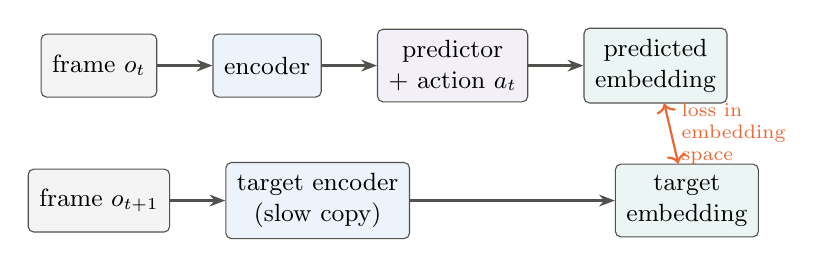
\begin{tikzpicture}[node distance=4mm and 7mm, every node/.style={font=\small}]
\node[bx=gray] (o) {frame $o_t$};
\node[bx=cA, right=of o] (e) {encoder};
\node[bx=cD, right=of e] (p) {predictor\\$+$ action $a_t$};
\node[bx=cC, right=of p] (zh) {predicted\\embedding};
\node[bx=gray, below=9mm of o] (o2) {frame $o_{t+1}$};
\node[bx=cA, right=of o2] (e2) {target encoder\\(slow copy)};
\node[bx=cC, right=26mm of e2] (z2) {target\\embedding};
\draw[arr] (o)--(e); \draw[arr] (e)--(p); \draw[arr] (p)--(zh); \draw[arr] (o2)--(e2); \draw[arr] (e2)--(z2);
\draw[<->, thick, cB] (zh)--(z2) node[midway,right,font=\scriptsize,align=left]{loss in\\embedding\\space};
\end{tikzpicture}
\caption{A JEPA-style world model predicts the \emph{embedding} of the next frame, not the frame itself. A pixel world model would instead decode back to an image $\hat o_{t+1}$ and compare pixels.}
\label{fig:jepa}
\end{figure}

\begin{paperbox}{Assran et al.\ (2025), ``V-JEPA 2: Self-Supervised Video Models Enable Understanding, Prediction and Planning'' (Meta)}
Pre-trains a JEPA video encoder on more than a million hours of internet video, with no actions and no labels. Then trains a small action-conditioned predictor, V-JEPA 2-AC, on top of the frozen encoder, using less than 62 hours of unlabelled robot-arm videos with their actions. Planning: given a goal image, use CEM to find the actions whose predicted embedding is closest to the goal's embedding. The authors report zero-shot pick-and-place on robot arms in labs where no data had been collected. Lesson: most of a world model can be learned from ordinary video; only a thin action-conditioned part needs robot data.
\end{paperbox}

\begin{paperbox}{Zhou, Pan, LeCun \& Pinto (ICML 2025), ``DINO-WM: World Models on Pre-trained Visual Features enable Zero-shot Planning''}
Uses frozen DINOv2 patch features as the latent state and trains only a transformer predictor of future patch features, from offline trajectories. Planning with CEM towards a goal image's features solves navigation and manipulation tasks at test time without expert demonstrations, reward models or task-specific training. A simple and reproducible starting point if you want to build your own world model.
\end{paperbox}

\begin{quizbox}
\begin{enumerate}[leftmargin=*]
\item In Figure~\ref{fig:cem}, why do the samples not end up on the obstacle even though the straight line from start to goal passes near it?
\item What does a JEPA lose compared with a pixel model, and what does it gain?
\item Why is a goal \emph{image} a convenient way to give a world-model planner a task?
\end{enumerate}
\emph{Answers: 1) samples near the bump have high cost and are never elites; 2) it loses the ability to show you a picture of the prediction, and gains efficiency by ignoring unpredictable detail; 3) the cost is just the distance between embeddings, so no reward function has to be designed.}
\end{quizbox}

% --------------------------------------------------------------------
\section{Video world models and world foundation models}
\label{sec:video}

At the other end of the spectrum are models that generate realistic video. They are trained on huge video collections, usually as diffusion or autoregressive transformers over video tokens, and conditioned on text or actions.
\begin{itemize}
\item \textbf{Genie} (Bruce et al., 2024, Google DeepMind): learned interactive 2-D game worlds from internet gameplay videos \emph{without action labels}. A latent action model inferred a small set of discrete ``actions'' from consecutive frames; the world model was then conditioned on them. This shows how a world model can learn controllability from video alone.
\item \textbf{UniSim} (Yang et al., 2023): a video model conditioned on actions and language, used as a simulator to train policies.
\item \textbf{Cosmos} (NVIDIA, 2025): a platform of open ``world foundation models'' (diffusion and autoregressive) intended for physical AI: generating synthetic training data and testing policies for robots and cars.
\item \textbf{Genie 3} (Google DeepMind, announced August 2025): generates interactive 3-D worlds from text in real time, at 720p and 24 frames per second, and stays consistent for several minutes. At the time of writing it is a research preview.
\end{itemize}

\begin{table}[h]
\centering\small
\begin{tabularx}{\linewidth}{@{}>{\raggedright\arraybackslash}p{3.3cm} >{\raggedright\arraybackslash}X >{\raggedright\arraybackslash}X@{}}
\toprule
 & Latent predictive models (Dreamer, TD-MPC2, DINO-WM, V-JEPA 2) & Pixel generative models (Genie, UniSim, Cosmos) \\
\midrule
Predicts & compact latent states or embeddings & images or video \\
Speed & fast enough for MPC in a control loop & slow; many network passes per frame \\
Best use & planning and policy learning & simulation, data generation, testing \\
Can a human inspect the prediction? & not directly (unless there is a decoder) & yes \\
Main weakness & needs care against trivial solutions; less general & physically wrong ``hallucinations''; drift over long horizons \\
\bottomrule
\end{tabularx}
\caption{The two families of world models.}
\label{tab:wmfam}
\end{table}

\begin{paperbox}{Alrasheed, Azam \& Akhtar (2026), ``The Planning Limits of Latent World Models''}
Tests when latent world models actually help planning. Finding: a world model is useful for planning only when the goal lies within, or slightly beyond, the trajectory it can imagine. Used inside that range, it improves a VLA by choosing among eight action candidates the VLA proposes; this raised success from 65\% to 77\% over 16 tasks. Lesson: today, the world model is best used as a \emph{critic of a policy's proposals} over short horizons, not as a stand-alone planner over long ones.
\end{paperbox}

\begin{quizbox}
\begin{enumerate}[leftmargin=*]
\item How can Genie learn which ``actions'' exist if its training videos have no action labels?
\item Which family of Table~\ref{tab:wmfam} would you use inside a 10~Hz drone planning loop on a ground-station GPU, and why?
\end{enumerate}
\emph{Answers: 1) a latent action model infers, from pairs of consecutive frames, a small discrete code that explains the change; those codes become the actions; 2) a latent predictive model, because it is fast enough; a pixel model can be used offline to generate training data or test scenes.}
\end{quizbox}

\part{Putting it together: drones and your thesis}
% ============================== PART V ==============================
\section{Combining VLAs and world models, and what exists for drones}
\label{sec:combine}

\subsection{The propose--imagine--verify loop}
Part III ended with a gap: a reasoning VLA can propose plans but cannot check their physics. Part IV ended with the matching strength: a world model can check a proposal over a short horizon but is a poor planner on its own. Put together, they give the loop in Figure~\ref{fig:verify}.

\begin{figure}[h]
\centering
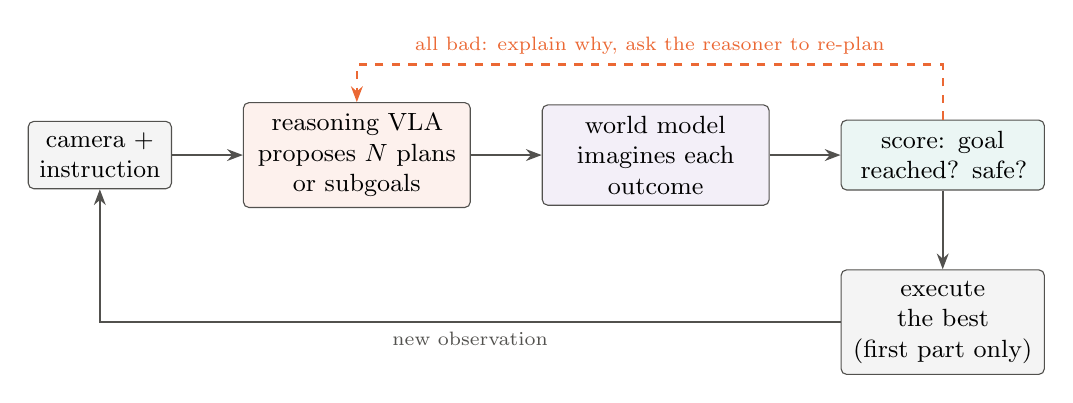
\begin{tikzpicture}[node distance=6mm and 9mm, every node/.style={font=\small}]
\node[bx=gray] (obs) {camera +\\instruction};
\node[bx=cB, right=of obs, text width=2.6cm] (vla) {reasoning VLA\\proposes $N$ plans\\or subgoals};
\node[bx=cD, right=of vla, text width=2.6cm] (wm) {world model\\imagines each\\outcome};
\node[bx=cC, right=of wm, text width=2.3cm] (sc) {score: goal\\reached? safe?};
\node[bx=gray, below=10mm of sc, text width=2.3cm] (ex) {execute the best\\(first part only)};
\draw[arr] (obs)--(vla); \draw[arr] (vla)--(wm); \draw[arr] (wm)--(sc); \draw[arr] (sc)--(ex);
\draw[darr] (sc.north) -- ++(0,0.7) -| node[pos=0.25,above,font=\scriptsize]{all bad: explain why, ask the reasoner to re-plan} (vla.north);
\draw[arr] (ex.west) -| node[pos=0.25,below,font=\scriptsize]{new observation} (obs.south);
\end{tikzpicture}
\caption{Propose, imagine, verify. The reasoning model supplies semantic candidates, the world model checks their physics, and failures are fed back to the reasoner. The dashed feedback arrow is the least explored part.}
\label{fig:verify}
\end{figure}

Recent papers implement parts of this loop:
\begin{itemize}
\item \textbf{Selecting among proposals:} the ``Planning Limits'' study (Alrasheed et al., 2026) lets a world model choose among 8 VLA candidates (65\% $\to$ 77\% success). \textbf{Pre-VLA} (2026) adds a verifier that rejects poor action chunks before they are executed or imagined.
\item \textbf{Foresight as guidance:} \textbf{ForeAct} (Zhang et al., 2026) generates imagined future views and subtask descriptions that steer a VLA step by step; the authors report 87.4\% average success on 11 real tasks against 46.5\% for $\pi_0$.
\item \textbf{Joint models:} CoT-VLA (Section~\ref{sec:rvla}) generates a subgoal image and then actions. In autonomous driving, DriveWorld-VLA and VLA-World (2026) unify world modelling and planning in one latent space and add ``what-if'' reasoning about candidate actions.
\end{itemize}

\subsection{What exists for drones}
\label{sec:drones}
\textbf{VLAs for drones.} RaceVLA and CognitiveDrone (Skoltech, 2025) were early VLA-controlled drones for racing and cognitive tasks. AerialVLA (2026) maps camera images and instructions to continuous flight commands. AutoFly (ICLR 2026) is an end-to-end VLA for navigation in the wild. \textbf{AirVLA} (Tucker et al., 2026, ``$\pi$, But Make It Fly'') took $\pi_0$, trained for fixed arms, to aerial manipulation. Its finding is important for you: the \emph{visual} knowledge transferred, but the \emph{flight dynamics} did not. A physics-aware guidance step at sampling time raised real pick-and-place success from 23\% to 50\%.

\textbf{World models for drones.} Dream to Fly (Romero et al., 2025) and the NTNU follow-up (Zanatta et al., 2026) use Dreamer world models for vision-based flight, without language.

\textbf{World models plus language for drones.} This combination appeared in mid-2026:
\begin{itemize}
\item \textbf{ImagineUAV} (Liu et al., 2026): a 1.3B latent video diffusion model imagines future views from the instruction; an action extractor turns them into 6-DoF motion; a kinodynamic planner makes the result collision-free. Evaluated on benchmarks and in real flights.
\item \textbf{WorldVLN} (Zhao et al., 2026): an autoregressive latent video model predicts short-term world states and converts them to waypoints; reported to transfer zero-shot to a real drone, with indoor and outdoor benchmarks.
\item \textbf{WorldFly} (Zheng et al., 2026): jointly generates future video and navigation actions with coupled flow matching, for dense urban canyons.
\end{itemize}

\begin{table}[h]
\centering\footnotesize
\begin{tabular}{@{}l c c c c c c@{}}
\toprule
 & language & reasoning & world model & real drone & safety & multi-drone\\
\midrule
Dream to Fly (2025) & -- & -- & \checkmark & \checkmark & -- & -- \\
AirVLA (2026) & \checkmark & -- & -- & \checkmark & partly & -- \\
AerialVLA, AutoFly (2026) & \checkmark & -- & -- & ? & -- & -- \\
ImagineUAV (2026) & \checkmark & -- & \checkmark & \checkmark & planner & -- \\
WorldVLN (2026) & \checkmark & -- & \checkmark & \checkmark & -- & -- \\
WorldFly (2026) & \checkmark & -- & \checkmark & ? & -- & -- \\
\bottomrule
\end{tabular}
\caption{What the closest drone papers combine, as far as their abstracts and summaries say. ``?'' means I could not tell from what I read; ``partly'' and ``planner'' mean a physics-based component, not a formal safety guarantee. Check the full papers before citing this table.}
\label{tab:drones}
\end{table}

\begin{opinionbox}
Three things look open, based on Table~\ref{tab:drones} and the papers above:
\begin{enumerate}[leftmargin=*]
\item \textbf{Explicit reasoning checked by a world model, with feedback.} The drone papers use the world model to \emph{generate} motion. None that I found has a reasoner that proposes subgoals in words, a world model that rejects the infeasible ones, and an explanation that goes back to the reasoner (the dashed arrow in Figure~\ref{fig:verify}).
\item \textbf{A formal safety layer under the learned layers.} Learned models give no guarantees. A control barrier function filter (Ames et al., 2019) between the learned commands and the flight controller would make the system provably keep its distance from obstacles, whatever the learned parts propose.
\item \textbf{Tiny drones and several drones.} The papers use drones that carry good cameras or a companion computer and fly alone. Indoor micro-drones that see only through a small camera and rely on a ground station, possibly in groups, are not covered.
\end{enumerate}
This field moves every month. Search again right before you write the proposal, and be ready for one of these gaps to close.
\end{opinionbox}

% --------------------------------------------------------------------
\section{From here to a thesis}

\subsection{A layered architecture}
Figure~\ref{fig:stack} shows how the pieces of these notes could stack on top of what you have already built. Each layer runs at its own rate and can be tested on its own.

\begin{figure}[h]
\centering
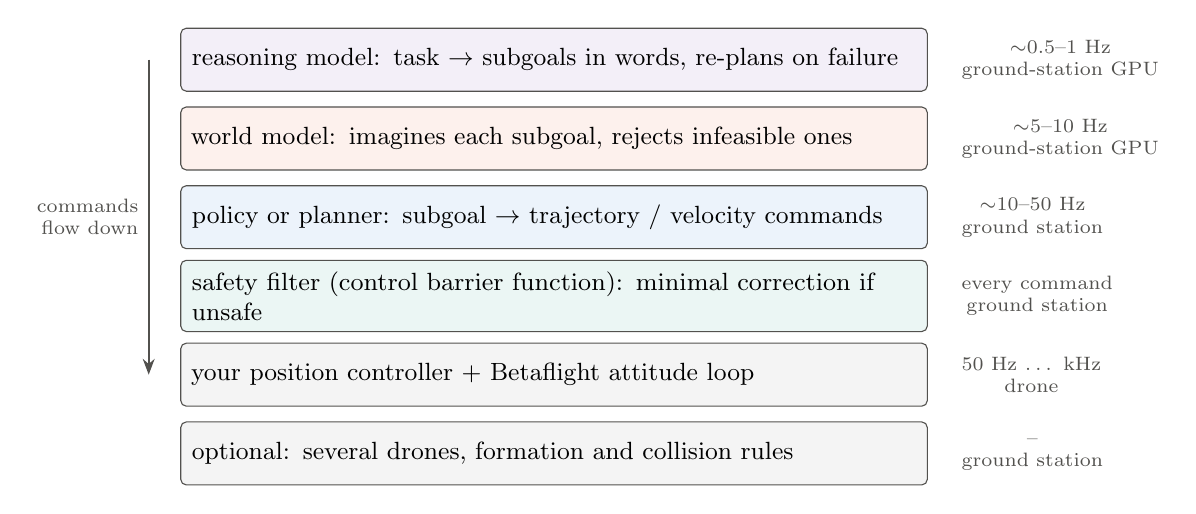
\begin{tikzpicture}[every node/.style={font=\small}]
\foreach \y/\c/\t/\r/\w in {
 5/cD/{reasoning model: task $\to$ subgoals in words, re-plans on failure}/{$\sim$0.5--1 Hz}/{ground-station GPU},
 4/cB/{world model: imagines each subgoal, rejects infeasible ones}/{$\sim$5--10 Hz}/{ground-station GPU},
 3/cA/{policy or planner: subgoal $\to$ trajectory / velocity commands}/{$\sim$10--50 Hz}/{ground station},
 2/cC/{safety filter (control barrier function): minimal correction if unsafe}/{every command}/{ground station},
 1/gray/{your position controller + Betaflight attitude loop}/{50 Hz $\dots$ kHz}/{drone},
 0/gray/{optional: several drones, formation and collision rules}/{--}/{ground station}}{
 \node[bx=\c, minimum width=9.4cm, text width=9.2cm, align=left, anchor=west] at (0,\y*1.0) {\t};
 \node[lbl, anchor=west] at (9.8,\y*1.0) {\r\\\w};
}
\draw[arr] (-0.4,5)--(-0.4,1) node[midway,left,font=\scriptsize,align=right]{commands\\flow down};
\end{tikzpicture}
\caption{A possible stack. The bottom two layers exist (or existed in your bachelor project); the learned layers sit on top, and the safety filter makes sure they cannot command anything dangerous.}
\label{fig:stack}
\end{figure}

\begin{opinionbox}
A research question that follows from Section~\ref{sec:combine}: \emph{Does verifying a reasoning model's subgoals with a learned world model, and feeding failures back to it, make long multi-step drone tasks more successful and safer than reasoning alone or a world model alone?} It gives clean experiments, with four variants: VLA only, reasoning VLA, world-model planner, and the full loop. It can be tested in simulation first and on small indoor drones at the end. The architecture uses pretrained models (a VLM for reasoning, a DINO-WM- or V-JEPA-style world model), so the work is in connecting, fine-tuning and evaluating them, which fits a master's thesis.
\end{opinionbox}

\begin{probbox}{how many trials you need to compare two success rates}
Each trial succeeds or fails, a Bernoulli variable with success probability $p$ and variance $p(1-p)$. The measured success rate $\hat p$ over $n$ independent trials is a mean of $n$ such variables, so $\E[\hat p]=p$ and $\mathrm{Var}(\hat p)=p(1-p)/n$. Its \textbf{standard error} is $\sqrt{p(1-p)/n}$. By the central limit theorem, $\hat p$ is roughly Gaussian for large $n$, so about 95\% of the time it lies within $1.96$ standard errors of $p$.

\textbf{Difference of two variants} measured on separate trials: variances add, so
\[
\mathrm{SE}(\hat p_2-\hat p_1)=\sqrt{\frac{p_1(1-p_1)}{n_1}+\frac{p_2(1-p_2)}{n_2}} .
\]
\textbf{Example.} 65\% versus 77\%, as in the Planning Limits paper, with $n=100$ trials each: $\mathrm{SE}=\sqrt{(0.2275+0.1771)/100}=0.064$, and the difference $0.12$ is $1.89$ standard errors, just short of the usual $1.96$. For it to pass you need $n\ge0.4046\,(1.96/0.12)^2\approx108$ trials per variant. With 20 trials per variant (common in real-robot papers) the standard error is about $0.14$, larger than the effect. Plan your drone experiments with this in mind: run many trials in simulation, and use the real flights to show that the result transfers.
\end{probbox}

\subsection{Skills, in the order you need them}
\begin{enumerate}
\item \textbf{PyTorch basics.} Write an MLP with autograd and train it on a toy problem. Re-derive Figure~\ref{fig:backprop} with \texttt{loss.backward()}.
\item \textbf{A transformer from scratch.} Andrej Karpathy's ``nanoGPT'' and his video ``Let's build GPT'' are the standard route. After that, Section~\ref{sec:transformer} will feel obvious.
\item \textbf{Behaviour cloning and diffusion policies.} Train a small diffusion or flow-matching policy on a simulated task; reproduce Figure~\ref{fig:bimodal} with it.
\item \textbf{Fine-tune an open VLA.} OpenVLA or $\pi_0$ (Physical Intelligence's open-source \texttt{openpi}) with LoRA on a simulated benchmark such as LIBERO.
\item \textbf{A world model.} Train DINO-WM or a small Dreamer on a simple environment, then plan with your own CEM (Figure~\ref{fig:cem}).
\item \textbf{A drone simulator.} For example a PyBullet-based quadrotor gym or NVIDIA Isaac Lab, with your controller in the loop.
\item \textbf{Safety filters.} Control barrier functions as a quadratic program; the 2019 tutorial by Ames et al.\ is in your Relevant Papers folder.
\end{enumerate}

\subsection{Reading list}
\textbf{Core (read in this order):}
\begin{enumerate}
\item Vaswani et al.\ (2017), \emph{Attention Is All You Need}: the transformer.
\item Dosovitskiy et al.\ (2021), \emph{ViT}; and skim Radford et al.\ (2021), \emph{CLIP}.
\item Chi et al.\ (2023), \emph{Diffusion Policy}: why generative policies.
\item Kim et al.\ (2024), \emph{OpenVLA}: the clearest open VLA.
\item Black et al.\ (2024), \emph{$\pi_0$}: the standard architecture today.
\item Zawalski et al.\ (2024), \emph{ECoT}: reasoning in a VLA.
\item Shi et al.\ (2025), \emph{Hi Robot}: hierarchical reasoning.
\item Hafner et al.\ (2023), \emph{DreamerV3}: latent world models and imagination training.
\item Zhou et al.\ (2025), \emph{DINO-WM}, and Assran et al.\ (2025), \emph{V-JEPA 2}: planning with pretrained features.
\item Alrasheed et al.\ (2026), \emph{The Planning Limits of Latent World Models}: when it helps.
\item Romero et al.\ (2025), \emph{Dream to Fly}; then ImagineUAV and WorldVLN (2026): the drone state of the art.
\end{enumerate}
\textbf{Surveys to keep at hand:} the VLA survey by Ma et al.\ (arXiv 2405.14093) and the 2025 review ``VLA Models for Robotics: A Review Towards Real-World Applications'' (arXiv 2510.07077); for world models, ``Understanding World or Predicting Future?'' (arXiv 2411.14499).

\begin{quizbox}
\begin{enumerate}[leftmargin=*]
\item For each layer of Figure~\ref{fig:stack}, which section of these notes explains it?
\item What would a fair baseline be for the full propose--imagine--verify loop?
\end{enumerate}
\emph{Answers: 1) reasoning: \S9; world model: \S10--13; policy/planner: \S7--8 and \S12; safety filter: outside these notes (Ames et al.); controller: your own work; 2) the same system with each component removed in turn, run on the same tasks and the same simulator with the same compute budget.}
\end{quizbox}

% --------------------------------------------------------------------
\section*{Sources}
\addcontentsline{toc}{section}{Sources}
\small
Papers are grouped by part. arXiv numbers are given where I am sure of them. The 2026 papers were checked against their arXiv abstracts or summaries, not read in full.

\textbf{Deep-learning background.}
Kingma \& Ba, Adam, arXiv 1412.6980.
He et al., ResNet, arXiv 1512.03385.
Vaswani et al., Attention Is All You Need, arXiv 1706.03762.
Dosovitskiy et al., ViT, arXiv 2010.11929.
Radford et al., CLIP, arXiv 2103.00020.
Zhai et al., SigLIP, arXiv 2303.15343.
Oquab et al., DINOv2, arXiv 2304.07193.
Liu et al., LLaVA, arXiv 2304.08485.
Hu et al., LoRA, arXiv 2106.09685.
Wei et al., Chain-of-Thought Prompting, arXiv 2201.11903.
Ouyang et al., InstructGPT/RLHF, arXiv 2203.02155.
DeepSeek-AI, DeepSeek-R1, arXiv 2501.12948.
Ho et al., DDPM, arXiv 2006.11239.
Lipman et al., Flow Matching, arXiv 2210.02747.

\textbf{Robot learning.}
Schulman et al., PPO, arXiv 1707.06347.
Ross \& Bagnell, Efficient Reductions for Imitation Learning, AISTATS 2010.
Ross, Gordon \& Bagnell, DAgger, arXiv 1011.0686.
Zhao et al., ACT/ALOHA, arXiv 2304.13705.
Chi et al., Diffusion Policy, arXiv 2303.04137.
Open X-Embodiment Collaboration, arXiv 2310.08864.
Khazatsky et al., DROID, arXiv 2403.12945.
Kaufmann et al., Champion-level drone racing using deep RL, Nature 620 (2023).
Ames et al., Control Barrier Functions: Theory and Applications, arXiv 1903.11199.

\textbf{VLAs and reasoning VLAs.}
Brohan et al., RT-1, arXiv 2212.06817.
Brohan et al., RT-2, arXiv 2307.15818.
Octo Model Team, Octo, arXiv 2405.12213.
Kim et al., OpenVLA, arXiv 2406.09246.
Black et al., $\pi_0$, arXiv 2410.24164.
Physical Intelligence, $\pi_{0.5}$, arXiv 2504.16054.
Pertsch et al., FAST, arXiv 2501.09747.
NVIDIA, GR00T N1, arXiv 2503.14734.
Figure AI, Helix (company report, 2025).
Google DeepMind, Gemini Robotics and Gemini Robotics 1.5 (technical reports, 2025).
Zawalski et al., ECoT, arXiv 2407.08693.
Shi et al., Hi Robot, arXiv 2502.19417.
Zhao et al., CoT-VLA, arXiv 2503.22020 (CVPR 2025).
Huang et al., ThinkAct, arXiv 2507.16815.
Zhong et al., ACoT-VLA, arXiv 2601.11404 (CVPR 2026).
Ma et al., A Survey on VLA Models for Embodied AI, arXiv 2405.14093.
VLA Models for Robotics: A Review Towards Real-World Applications, arXiv 2510.07077.

\textbf{World models.}
Ha \& Schmidhuber, World Models, arXiv 1803.10122.
Hafner et al., PlaNet, arXiv 1811.04551.
Hafner et al., Dreamer, arXiv 1912.01603.
Hafner et al., DreamerV3, arXiv 2301.04104 (Nature, 2025).
Schrittwieser et al., MuZero, arXiv 1911.08265.
Hansen et al., TD-MPC2, arXiv 2310.16828.
LeCun, A Path Towards Autonomous Machine Intelligence (JEPA position paper), OpenReview 2022.
Assran et al., V-JEPA 2, arXiv 2506.09985.
Zhou, Pan, LeCun \& Pinto, DINO-WM, arXiv 2411.04983 (ICML 2025).
Bruce et al., Genie, arXiv 2402.15391.
Yang et al., UniSim, arXiv 2310.06114.
NVIDIA, Cosmos World Foundation Model Platform, arXiv 2501.03575.
Google DeepMind, Genie 3 (announcement, August 2025).
Understanding World or Predicting Future? A Comprehensive Survey of World Models, arXiv 2411.14499.
Alrasheed, Azam \& Akhtar, The Planning Limits of Latent World Models, arXiv 2609.39235.

\textbf{Combining VLAs, world models and drones.}
Zhang et al., ForeAct, arXiv 2602.12322.
Pre-VLA, arXiv 2605.22446.
DriveWorld-VLA, arXiv 2602.06521; VLA-World, arXiv 2604.09059.
Romero et al., Dream to Fly, arXiv 2501.14377.
Zanatta, Malczyk \& Alexis, Generalization of World Models under Environmental Variability, arXiv 2606.05015.
Serpiva et al., RaceVLA (2025); Lykov et al., CognitiveDrone (2025).
AerialVLA, arXiv 2603.14363.
AutoFly, arXiv 2602.09657 (ICLR 2026).
Tucker et al., $\pi$, But Make It Fly (AirVLA), arXiv 2603.25038.
Liu et al., ImagineUAV, arXiv 2606.01205.
Zhao et al., WorldVLN, arXiv 2605.15964.
Zheng et al., WorldFly, arXiv 2606.06147.


\end{document}
